%%=====================================================================
%%  TERM PAPER -- VERSION v0.1  (DRAFT)
%%  "Microarchitectural Security in Modern RISC-V Processors: Cache and
%%   Speculative-Execution Attacks, Defenses, and Performance Trade-offs"
%%
%%  SINGLE-FILE SUBMISSION POLICY
%%  ----------------------------------------------------------------
%%  This is ONE self-contained .tex file. It contains:
%%    * the complete text of the report,
%%    * every figure, drawn programmatically with TikZ / CircuiTikZ /
%%      pgfplots / tikz-timing (no external image files, no \includegraphics),
%%    * the complete BibTeX database, embedded below with `filecontents*`.
%%
%%  The bibliography is exported from Zotero and pasted into the
%%  filecontents* block below. At compile time LaTeX writes it out as
%%  refs.bib, so BibTeX can run -- but NOTHING except this .tex file is
%%  ever submitted.
%%
%%  HOW TO COMPILE (produces the accompanying PDF):
%%      pdflatex   RISCV_Microarch_Security_TermPaper_v0.1.tex
%%      bibtex     RISCV_Microarch_Security_TermPaper_v0.1
%%      makeindex  RISCV_Microarch_Security_TermPaper_v0.1.idx
%%      pdflatex   RISCV_Microarch_Security_TermPaper_v0.1.tex
%%      pdflatex   RISCV_Microarch_Security_TermPaper_v0.1.tex
%%  or simply:   latexmk -pdf RISCV_Microarch_Security_TermPaper_v0.1.tex
%%  (latexmk runs bibtex and makeindex itself. The glossary needs no external
%%   tool: glossaries is used in \makenoidxglossaries mode and LaTeX sorts it.)
%%=====================================================================

\begin{filecontents*}[overwrite]{refs.bib}
@book{sarangi2025basic,
  author    = {Sarangi, Smruti R.},
  title     = {Basic Computer Architecture},
  year      = {2025},
  month     = {October},
  publisher = {Self-published (open access)},
  note      = {Version 3.09; prescribed textbook},
  url       = {https://srsarangi.github.io/archbook/archbook.pdf}
}

@book{hennessy2019quantitative,
  author    = {Hennessy, John L. and Patterson, David A.},
  title     = {Computer Architecture: A Quantitative Approach},
  edition   = {6th},
  publisher = {Morgan Kaufmann},
  year      = {2019}
}

@misc{riscv-unpriv,
  author       = {Waterman, Andrew and Asanovi{\'c}, Krste},
  title        = {The {RISC-V} Instruction Set Manual, Volume {I}: Unprivileged {ISA}},
  howpublished = {RISC-V International},
  year         = {2019},
  note         = {Document version 20191213}
}

@misc{riscv-priv,
  author       = {Waterman, Andrew and Asanovi{\'c}, Krste and Hauser, John},
  title        = {The {RISC-V} Instruction Set Manual, Volume {II}: Privileged Architecture},
  howpublished = {RISC-V International},
  year         = {2021},
  note         = {Document version 20211203}
}

@misc{riscv-crypto,
  author       = {{RISC-V International}},
  title        = {{RISC-V} Cryptography Extensions Volume {I}: Scalar {\&} Entropy Source Instructions},
  howpublished = {RISC-V International},
  year         = {2022},
  note         = {Includes the Zkt data-independent execution latency extension}
}

@misc{riscv-cfi,
  author       = {{RISC-V International}},
  title        = {{RISC-V} Control-Flow Integrity: Shadow Stacks ({Zicfiss}) and Landing Pads ({Zicfilp})},
  howpublished = {RISC-V International Specification},
  year         = {2024}
}

@article{smith1988precise,
  author  = {Smith, James E. and Pleszkun, Andrew R.},
  title   = {Implementing Precise Interrupts in Pipelined Processors},
  journal = {IEEE Transactions on Computers},
  volume  = {37},
  number  = {5},
  year    = {1988},
  pages     = {562--573},
  doi       = {10.1109/12.4607}
}

@inproceedings{kocher2019spectre,
  author    = {Kocher, Paul and Horn, Jann and Fogh, Anders and Genkin, Daniel and
               Gruss, Daniel and Haas, Werner and Hamburg, Mike and Lipp, Moritz and
               Mangard, Stefan and Prescher, Thomas and Schwarz, Michael and Yarom, Yuval},
  title     = {Spectre Attacks: Exploiting Speculative Execution},
  booktitle = {IEEE Symposium on Security and Privacy (S\&P)},
  year      = {2019},
  pages     = {1--19},
  doi       = {10.1109/SP.2019.00002}
}

@inproceedings{lipp2018meltdown,
  author    = {Lipp, Moritz and Schwarz, Michael and Gruss, Daniel and Prescher, Thomas and
               Haas, Werner and Fogh, Anders and Horn, Jann and Mangard, Stefan and
               Kocher, Paul and Genkin, Daniel and Yarom, Yuval and Hamburg, Mike},
  title     = {Meltdown: Reading Kernel Memory from User Space},
  booktitle = {USENIX Security Symposium},
  year      = {2018},
  pages     = {973--990}
}

@inproceedings{yarom2014flushreload,
  author    = {Yarom, Yuval and Falkner, Katrina},
  title     = {{FLUSH+RELOAD}: A High Resolution, Low Noise, {L3} Cache Side-Channel Attack},
  booktitle = {USENIX Security Symposium},
  year      = {2014},
  pages     = {719--732}
}

@inproceedings{osvik2006cache,
  author    = {Osvik, Dag Arne and Shamir, Adi and Tromer, Eran},
  title     = {Cache Attacks and Countermeasures: The Case of {AES}},
  booktitle = {Topics in Cryptology (CT-RSA)},
  year      = {2006},
  pages     = {1--20},
  doi       = {10.1007/11605805_1}
}

@misc{percival2005cache,
  author       = {Percival, Colin},
  title        = {Cache Missing for Fun and Profit},
  howpublished = {BSDCan},
  year         = {2005}
}

@misc{bernstein2005aes,
  author       = {Bernstein, Daniel J.},
  title        = {Cache-Timing Attacks on {AES}},
  howpublished = {Technical report, University of Illinois at Chicago},
  year         = {2005}
}

@inproceedings{kocher1996timing,
  author    = {Kocher, Paul C.},
  title     = {Timing Attacks on Implementations of {Diffie-Hellman}, {RSA}, {DSS}, and Other Systems},
  booktitle = {Advances in Cryptology (CRYPTO)},
  year      = {1996},
  pages     = {104--113},
  doi       = {10.1007/3-540-68697-5_9}
}

@inproceedings{liu2015llc,
  author    = {Liu, Fangfei and Yarom, Yuval and Ge, Qian and Heiser, Gernot and Lee, Ruby B.},
  title     = {Last-Level Cache Side-Channel Attacks Are Practical},
  booktitle = {IEEE Symposium on Security and Privacy (S\&P)},
  year      = {2015},
  pages     = {605--622},
  doi       = {10.1109/SP.2015.43}
}

@inproceedings{gruss2016flushflush,
  author    = {Gruss, Daniel and Maurice, Cl{\'e}mentine and Wagner, Klaus and Mangard, Stefan},
  title     = {{Flush+Flush}: A Fast and Stealthy Cache Attack},
  booktitle = {Detection of Intrusions and Malware, and Vulnerability Assessment (DIMVA)},
  year      = {2016},
  pages     = {279--299},
  doi       = {10.1007/978-3-319-40667-1_14}
}

@inproceedings{gruss2016prefetch,
  author    = {Gruss, Daniel and Maurice, Cl{\'e}mentine and Fogh, Anders and Lipp, Moritz and Mangard, Stefan},
  title     = {Prefetch Side-Channel Attacks: Bypassing {SMAP} and Kernel {ASLR}},
  booktitle = {ACM Conference on Computer and Communications Security (CCS)},
  year      = {2016},
  pages     = {368--379},
  doi       = {10.1145/2976749.2978356}
}

@inproceedings{canella2019systematic,
  author    = {Canella, Claudio and Van Bulck, Jo and Schwarz, Michael and Lipp, Moritz and
               von Berg, Benjamin and Ortner, Philipp and Piessens, Frank and Evtyushkin, Dmitry and
               Gruss, Daniel},
  title     = {A Systematic Evaluation of Transient Execution Attacks and Defenses},
  booktitle = {USENIX Security Symposium},
  year      = {2019},
  pages     = {249--266}
}

@inproceedings{vanbulck2018foreshadow,
  author    = {Van Bulck, Jo and Minkin, Marina and Weisse, Ofir and Genkin, Daniel and
               Kasikci, Baris and Piessens, Frank and Silberstein, Mark and Wenisch, Thomas F. and
               Yarom, Yuval and Strackx, Raoul},
  title     = {Foreshadow: Extracting the Keys to the {Intel SGX} Kingdom with Transient Out-of-Order Execution},
  booktitle = {USENIX Security Symposium},
  year      = {2018},
  pages     = {991--1008}
}

@inproceedings{schwarz2019zombieload,
  author    = {Schwarz, Michael and Lipp, Moritz and Moghimi, Daniel and Van Bulck, Jo and
               Stecklina, Julian and Prescher, Thomas and Gruss, Daniel},
  title     = {{ZombieLoad}: Cross-Privilege-Boundary Data Sampling},
  booktitle = {ACM Conference on Computer and Communications Security (CCS)},
  year      = {2019},
  pages     = {753--768},
  doi       = {10.1145/3319535.3354252}
}

@inproceedings{vanschaik2019ridl,
  author    = {van Schaik, Stephan and Milburn, Alyssa and {\"O}sterlund, Sebastian and
               Frigo, Pietro and Maisuradze, Giorgi and Razavi, Kaveh and Bos, Herbert and
               Giuffrida, Cristiano},
  title     = {{RIDL}: Rogue In-Flight Data Load},
  booktitle = {IEEE Symposium on Security and Privacy (S\&P)},
  year      = {2019},
  pages     = {88--105},
  doi       = {10.1109/SP.2019.00087}
}

@inproceedings{wikner2022retbleed,
  author    = {Wikner, Johannes and Razavi, Kaveh},
  title     = {{RETBLEED}: Arbitrary Speculative Code Execution with Return Instructions},
  booktitle = {USENIX Security Symposium},
  year      = {2022},
  pages     = {3825--3842}
}

@inproceedings{barberis2022bhi,
  author    = {Barberis, Enrico and Frigo, Pietro and Muench, Marius and Bos, Herbert and Giuffrida, Cristiano},
  title     = {Branch History Injection: On the Effectiveness of Hardware Mitigations Against Cross-Privilege {Spectre-v2} Attacks},
  booktitle = {USENIX Security Symposium},
  year      = {2022},
  pages     = {971--988}
}

@inproceedings{evtyushkin2018branchscope,
  author    = {Evtyushkin, Dmitry and Riley, Ryan and Abu-Ghazaleh, Nael and Ponomarev, Dmitry},
  title     = {{BranchScope}: A New Side-Channel Attack on Directional Branch Predictor},
  booktitle = {ACM International Conference on Architectural Support for Programming Languages and Operating Systems (ASPLOS)},
  year      = {2018},
  pages     = {693--707},
  doi       = {10.1145/3173162.3173204}
}

@inproceedings{gras2018tlbleed,
  author    = {Gras, Ben and Razavi, Kaveh and Bos, Herbert and Giuffrida, Cristiano},
  title     = {Translation Leak-aside Buffer: Defeating Cache Side-Channel Protections with {TLB} Attacks},
  booktitle = {USENIX Security Symposium},
  year      = {2018},
  pages     = {955--972}
}

@inproceedings{behnia2021interference,
  author    = {Behnia, Mohammad and Sahu, Prateek and Paccagnella, Riccardo and Yu, Jiyong and
               Zhao, Zirui Neil and Zou, Xiang and Unterluggauer, Thomas and Torrellas, Josep and
               Rozas, Carlos and Morrison, Adam and Mckeen, Frank and Liu, Fangfei and
               Gabor, Ron and Fletcher, Christopher W. and Basak, Abhishek and Alameldeen, Alaa},
  title     = {Speculative Interference Attacks: Breaking Invisible Speculation Schemes},
  booktitle = {ACM International Conference on Architectural Support for Programming Languages and Operating Systems (ASPLOS)},
  year      = {2021},
  pages     = {1046--1060},
  doi       = {10.1145/3445814.3446708}
}

@inproceedings{kim2014rowhammer,
  author    = {Kim, Yoongu and Daly, Ross and Kim, Jeremie and Fallin, Chris and Lee, Ji Hye and
               Lee, Donghyuk and Wilkerson, Chris and Lai, Konrad and Mutlu, Onur},
  title     = {Flipping Bits in Memory Without Accessing Them: An Experimental Study of {DRAM} Disturbance Errors},
  booktitle = {International Symposium on Computer Architecture (ISCA)},
  year      = {2014},
  pages     = {361--372},
  doi       = {10.1109/ISCA.2014.6853210}
}

@inproceedings{kiriansky2018dawg,
  author    = {Kiriansky, Vladimir and Lebedev, Ilia and Amarasinghe, Saman and Devadas, Srinivas and Emer, Joel},
  title     = {{DAWG}: A Defense Against Cache Timing Attacks in Speculative Execution Processors},
  booktitle = {IEEE/ACM International Symposium on Microarchitecture (MICRO)},
  year      = {2018},
  pages     = {974--987},
  doi       = {10.1109/MICRO.2018.00083}
}

@inproceedings{qureshi2018ceaser,
  author    = {Qureshi, Moinuddin K.},
  title     = {{CEASER}: Mitigating Conflict-Based Cache Attacks via Encrypted-Address and Remapping},
  booktitle = {IEEE/ACM International Symposium on Microarchitecture (MICRO)},
  year      = {2018},
  pages     = {775--787},
  doi       = {10.1109/MICRO.2018.00068}
}

@inproceedings{qureshi2019ceasers,
  author    = {Qureshi, Moinuddin K.},
  title     = {New Attacks and Defense for Encrypted-Address Cache},
  booktitle = {International Symposium on Computer Architecture (ISCA)},
  year      = {2019},
  pages     = {360--371},
  doi       = {10.1145/3307650.3322246}
}

@inproceedings{werner2019scattercache,
  author    = {Werner, Mario and Unterluggauer, Thomas and Giner, Lukas and Schwarz, Michael and
               Gruss, Daniel and Mangard, Stefan},
  title     = {{ScatterCache}: Thwarting Cache Attacks via Cache Set Randomization},
  booktitle = {USENIX Security Symposium},
  year      = {2019},
  pages     = {675--692}
}

@inproceedings{saileshwar2021mirage,
  author    = {Saileshwar, Gururaj and Qureshi, Moinuddin K.},
  title     = {{MIRAGE}: Mitigating Conflict-Based Cache Attacks with a Practical Fully-Associative Design},
  booktitle = {USENIX Security Symposium},
  year      = {2021},
  pages     = {1379--1396}
}

@inproceedings{yan2018invisispec,
  author    = {Yan, Mengjia and Choi, Jiho and Skarlatos, Dimitrios and Morrison, Adam and
               Fletcher, Christopher W. and Torrellas, Josep},
  title     = {{InvisiSpec}: Making Speculative Execution Invisible in the Cache Hierarchy},
  booktitle = {IEEE/ACM International Symposium on Microarchitecture (MICRO)},
  year      = {2018},
  pages     = {428--441},
  doi       = {10.1109/MICRO.2018.00042}
}

@inproceedings{khasawneh2019safespec,
  author    = {Khasawneh, Khaled N. and Koruyeh, Esmaeil Mohammadian and Song, Chengyu and
               Evtyushkin, Dmitry and Ponomarev, Dmitry and Abu-Ghazaleh, Nael},
  title     = {{SafeSpec}: Banishing the Spectre of a Meltdown with Leakage-Free Speculation},
  booktitle = {ACM/IEEE Design Automation Conference (DAC)},
  year      = {2019},
  pages     = {60},
  doi       = {10.1145/3316781.3317903}
}

@inproceedings{saileshwar2019cleanupspec,
  author    = {Saileshwar, Gururaj and Qureshi, Moinuddin K.},
  title     = {{CleanupSpec}: An ``Undo'' Approach to Safe Speculation},
  booktitle = {IEEE/ACM International Symposium on Microarchitecture (MICRO)},
  year      = {2019},
  pages     = {73--86},
  doi       = {10.1145/3352460.3358314}
}

@inproceedings{yu2019stt,
  author    = {Yu, Jiyong and Yan, Mengjia and Khyzha, Artem and Morrison, Adam and
               Torrellas, Josep and Fletcher, Christopher W.},
  title     = {Speculative Taint Tracking ({STT}): A Comprehensive Protection for Speculatively Accessed Data},
  booktitle = {IEEE/ACM International Symposium on Microarchitecture (MICRO)},
  year      = {2019},
  pages     = {954--968},
  doi       = {10.1145/3352460.3358274}
}

@inproceedings{choudhary2021spt,
  author    = {Choudhary, Rutvik and Yu, Jiyong and Fletcher, Christopher W. and Morrison, Adam},
  title     = {Speculative Privacy Tracking ({SPT}): Leaking Information From Speculative Execution Without Compromising Privacy},
  booktitle = {IEEE/ACM International Symposium on Microarchitecture (MICRO)},
  year      = {2021},
  pages     = {607--622},
  doi       = {10.1145/3466752.3480068}
}

@inproceedings{weisse2019nda,
  author    = {Weisse, Ofir and Neal, Ian and Loughlin, Kevin and Wenisch, Thomas F. and Kasikci, Baris},
  title     = {{NDA}: Preventing Speculative Execution Attacks at Their Source},
  booktitle = {IEEE/ACM International Symposium on Microarchitecture (MICRO)},
  year      = {2019},
  pages     = {572--586},
  doi       = {10.1145/3352460.3358306}
}

@inproceedings{sakalis2019delay,
  author    = {Sakalis, Christos and Kaxiras, Stefanos and Ros, Alberto and Jimborean, Alexandra and
               Sj{\"a}lander, Magnus},
  title     = {Efficient Invisible Speculative Execution Through Selective Delay and Value Prediction},
  booktitle = {International Symposium on Computer Architecture (ISCA)},
  year      = {2019},
  pages     = {723--735},
  doi       = {10.1145/3307650.3322216}
}

@inproceedings{ainsworth2020muontrap,
  author    = {Ainsworth, Sam and Jones, Timothy M.},
  title     = {{MuonTrap}: Preventing Cross-Domain {Spectre-Like} Attacks by Capturing Speculative State},
  booktitle = {International Symposium on Computer Architecture (ISCA)},
  year      = {2020},
  pages     = {132--144},
  doi       = {10.1109/ISCA45697.2020.00022}
}

@inproceedings{ainsworth2021ghostminion,
  author    = {Ainsworth, Sam},
  title     = {{GhostMinion}: A Strictness-Ordered Cache System for {Spectre} Mitigation},
  booktitle = {IEEE/ACM International Symposium on Microarchitecture (MICRO)},
  year      = {2021},
  pages     = {592--606},
  doi       = {10.1145/3466752.3480074}
}

@inproceedings{bourgeat2019mi6,
  author    = {Bourgeat, Thomas and Lebedev, Ilia and Wright, Andrew and Zhang, Sizhuo and
               Arvind and Devadas, Srinivas},
  title     = {{MI6}: Secure Enclaves in a Speculative Out-of-Order Processor},
  booktitle = {IEEE/ACM International Symposium on Microarchitecture (MICRO)},
  year      = {2019},
  pages     = {42--56},
  doi       = {10.1145/3352460.3358310}
}

@inproceedings{costan2016sanctum,
  author    = {Costan, Victor and Lebedev, Ilia and Devadas, Srinivas},
  title     = {Sanctum: Minimal Hardware Extensions for Strong Software Isolation},
  booktitle = {USENIX Security Symposium},
  year      = {2016},
  pages     = {857--874}
}

@inproceedings{lee2020keystone,
  author    = {Lee, Dayeol and Kohlbrenner, David and Shinde, Shweta and Asanovi{\'c}, Krste and Song, Dawn},
  title     = {Keystone: An Open Framework for Architecting Trusted Execution Environments},
  booktitle = {European Conference on Computer Systems (EuroSys)},
  year      = {2020},
  pages     = {38:1--38:16},
  doi       = {10.1145/3342195.3387532}
}

@inproceedings{wistoff2021fencet,
  author    = {Wistoff, Nils and Schneider, Moritz and G{\"u}rkaynak, Frank K. and Benini, Luca and Heiser, Gernot},
  title     = {Microarchitectural Timing Channels and Their Prevention on an Open-Source 64-bit {RISC-V} Core},
  booktitle = {Design, Automation and Test in Europe (DATE)},
  year      = {2021},
  pages     = {627--632},
  doi       = {10.23919/DATE51398.2021.9474214}
}

@techreport{asanovic2016rocket,
  author      = {Asanovi{\'c}, Krste and Avizienis, Rimas and Bachrach, Jonathan and Beamer, Scott and others},
  title       = {The Rocket Chip Generator},
  institution = {EECS Department, University of California, Berkeley},
  number      = {UCB/EECS-2016-17},
  year        = {2016}
}

@inproceedings{zhao2020sonicboom,
  author    = {Zhao, Jerry and Korpan, Ben and Gonzalez, Abraham and Asanovi{\'c}, Krste},
  title     = {{SonicBOOM}: The {3rd} Generation {Berkeley} Out-of-Order Machine},
  booktitle = {Fourth Workshop on Computer Architecture Research with RISC-V (CARRV)},
  year      = {2020}
}

@article{zaruba2019ariane,
  author  = {Zaruba, Florian and Benini, Luca},
  title   = {The Cost of Application-Class Processing: Energy and Performance Analysis of a {Linux}-Ready 1.7-{GHz} 64-Bit {RISC-V} Core in 22-nm {FDSOI} Technology},
  journal = {IEEE Transactions on Very Large Scale Integration (VLSI) Systems},
  volume  = {27},
  number  = {11},
  year    = {2019},
  pages     = {2629--2640},
  doi       = {10.1109/TVLSI.2019.2926114}
}

@inproceedings{gonzalez2019replicating,
  author    = {Gonzalez, Abraham and Korpan, Ben and Zhao, Jerry and Younis, Ed and Asanovi{\'c}, Krste},
  title     = {Replicating and Mitigating {Spectre} Attacks on an Open Source {RISC-V} Microarchitecture},
  booktitle = {Third Workshop on Computer Architecture Research with RISC-V (CARRV)},
  year      = {2019}
}

@article{amid2020chipyard,
  author  = {Amid, Alon and Biancolin, David and Gonzalez, Abraham and Grubb, Daniel and
             Karandikar, Sagar and Liew, Harrison and Magyar, Albert and Mao, Howard and
             Ou, Albert and Pemberton, Nathan and Rigge, Paul and Schmidt, Colin and
             Wright, John and Zhao, Jerry and Shao, Yakun Sophia and Asanovi{\'c}, Krste and
             Nikoli{\'c}, Borivoje},
  title   = {Chipyard: Integrated Design, Simulation, and Implementation Framework for Custom {SoCs}},
  journal = {IEEE Micro},
  volume  = {40},
  number  = {4},
  year    = {2020},
  pages     = {10--21},
  doi       = {10.1109/MM.2020.2996616}
}

@inproceedings{karandikar2018firesim,
  author    = {Karandikar, Sagar and Mao, Howard and Kim, Donggyu and Biancolin, David and others},
  title     = {{FireSim}: {FPGA}-Accelerated Cycle-Exact Scale-Out System Simulation in the Public Cloud},
  booktitle = {International Symposium on Computer Architecture (ISCA)},
  year      = {2018},
  pages     = {29--42},
  doi       = {10.1109/ISCA.2018.00014}
}

@article{binkert2011gem5,
  author  = {Binkert, Nathan and Beckmann, Bradford and Black, Gabriel and Reinhardt, Steven K. and others},
  title   = {The {gem5} Simulator},
  journal = {ACM SIGARCH Computer Architecture News},
  volume  = {39},
  number  = {2},
  year    = {2011},
  pages     = {1--7},
  doi       = {10.1145/2024716.2024718}
}

@article{lowepower2020gem5,
  author  = {Lowe-Power, Jason and Ahmad, Abdul Mutaal and Akram, Ayaz and Alian, Mohammad and others},
  title   = {The {gem5} Simulator: Version 20.0+},
  journal = {arXiv preprint arXiv:2007.03152},
  year    = {2020}
}

@article{ge2018survey,
  author  = {Ge, Qian and Yarom, Yuval and Cock, David and Heiser, Gernot},
  title   = {A Survey of Microarchitectural Timing Attacks and Countermeasures on Contemporary Hardware},
  journal = {Journal of Cryptographic Engineering},
  volume  = {8},
  number  = {1},
  year    = {2018},
  pages     = {1--27},
  doi       = {10.1007/S13389-016-0141-6}
}

@inproceedings{wang2007newcache,
  author    = {Wang, Zhenghong and Lee, Ruby B.},
  title     = {New Cache Designs for Thwarting Software Cache-Based Side Channel Attacks},
  booktitle = {International Symposium on Computer Architecture (ISCA)},
  year      = {2007},
  pages     = {494--505},
  doi       = {10.1145/1250662.1250723}
}

@article{domnitser2012nonmono,
  author  = {Domnitser, Leonid and Jaleel, Aamer and Loew, Jason and Abu-Ghazaleh, Nael and Ponomarev, Dmitry},
  title   = {Non-Monopolizable Caches: Low-Complexity Mitigation of Cache Side Channel Attacks},
  journal = {ACM Transactions on Architecture and Code Optimization (TACO)},
  volume  = {8},
  number  = {4},
  year    = {2012},
  pages     = {35:1--35:21},
  doi       = {10.1145/2086696.2086714}
}

@inproceedings{liu2016catalyst,
  author    = {Liu, Fangfei and Ge, Qian and Yarom, Yuval and Mckeen, Frank and Rozas, Carlos and
               Heiser, Gernot and Lee, Ruby B.},
  title     = {{CATalyst}: Defeating Last-Level Cache Side Channel Attacks in Cloud Computing},
  booktitle = {IEEE International Symposium on High Performance Computer Architecture (HPCA)},
  year      = {2016},
  pages     = {406--418},
  doi       = {10.1109/HPCA.2016.7446082}
}

@inproceedings{deng2020benchmark,
  author    = {Deng, Shuwen and Xiong, Wenjie and Szefer, Jakub},
  title     = {A Benchmark Suite for Evaluating Caches' Vulnerability to Timing Attacks},
  booktitle = {ACM International Conference on Architectural Support for Programming Languages and Operating Systems (ASPLOS)},
  year      = {2020},
  pages     = {683--697},
  doi       = {10.1145/3373376.3378510}
}

@inproceedings{trippel2018checkmate,
  author    = {Trippel, Caroline and Lustig, Daniel and Martonosi, Margaret},
  title     = {{CheckMate}: Automated Synthesis of Hardware Exploits and Security Litmus Tests},
  booktitle = {IEEE/ACM International Symposium on Microarchitecture (MICRO)},
  year      = {2018},
  pages     = {947--960},
  doi       = {10.1109/MICRO.2018.00081}
}

@inproceedings{watson2015cheri,
  author    = {Watson, Robert N. M. and Woodruff, Jonathan and Neumann, Peter G. and Moore, Simon W. and others},
  title     = {{CHERI}: A Hybrid Capability-System Architecture for Scalable Software Compartmentalization},
  booktitle = {IEEE Symposium on Security and Privacy (S\&P)},
  year      = {2015},
  pages     = {20--37},
  doi       = {10.1109/SP.2015.9}
}

@misc{carruth2018slh,
  author       = {Carruth, Chandler},
  title        = {Speculative Load Hardening: A {Spectre} Variant \#1 Mitigation Technique},
  howpublished = {LLVM Project documentation},
  year         = {2018}
}

@misc{turner2018retpoline,
  author       = {Turner, Paul},
  title        = {Retpoline: A Software Construct for Preventing Branch-Target-Injection},
  howpublished = {Google technical whitepaper},
  year         = {2018}
}
\end{filecontents*}

%%=====================================================================
%% DOCUMENT CLASS AND PAGE GEOMETRY
%% Spec: A4 page, 1 inch margins all around, 12pt font,
%%       single-spaced lines.
%%=====================================================================
\documentclass[12pt,a4paper,oneside]{report}

\usepackage[a4paper,margin=1in,headheight=14pt]{geometry}

\usepackage[T1]{fontenc}
\usepackage[utf8]{inputenc}
%% Use Latin Modern where available; otherwise fall back to a Type-1 Times
%% family so that the file compiles on any TeX distribution.
\IfFileExists{lmodern.sty}{%
  \usepackage{lmodern}%
}{%
  \usepackage{mathptmx}%
  \usepackage[scaled=0.90]{helvet}%
  \usepackage{courier}%
}

\usepackage{setspace}
\singlespacing

%%=====================================================================
%% PACKAGES
%%=====================================================================
\usepackage{amsmath,amssymb,amsfonts}
\usepackage{microtype}
\usepackage{booktabs}
\usepackage{longtable}
\usepackage{tabularx}
\usepackage{multirow}
\usepackage{array}
\usepackage{enumitem}
\usepackage{xcolor}
\usepackage{graphicx}
\usepackage{listings}
\usepackage[most]{tcolorbox}
\usepackage{fancyhdr}
\usepackage{titlesec}
\usepackage[font=small,labelfont=bf,skip=6pt]{caption}
\usepackage{subcaption}
\usepackage{siunitx}
\usepackage{algorithm}
\usepackage{algpseudocode}
%% Numbered, IEEE-style citations, typeset with IEEEtranN.bst from the IEEEtran
%% package (TeX Live, MiKTeX, Overleaf all ship it). The style is selected
%% unconditionally at \bibliographystyle near the end of this file.
\usepackage[numbers,sort&compress]{natbib}

%% ---- Programmatic drawing stack (no external image files anywhere) ----
\usepackage{tikz}
\usetikzlibrary{arrows.meta,positioning,calc,shapes.geometric,shapes.misc,
                fit,backgrounds,decorations.pathreplacing,decorations.pathmorphing,
                patterns,matrix,chains,shadows.blur,through,intersections}
\usepackage{circuitikz}
\usepackage{pgfplots}
\pgfplotsset{compat=1.16}
\usepgfplotslibrary{groupplots,statistics,dateplot}
\usepackage{tikz-timing}   % WaveDrom-style timing diagrams, rendered in-file
\usepackage{forest}        % taxonomy trees

\usepackage[hidelinks,pdfusetitle]{hyperref}
\usepackage{cleveref}

%%=====================================================================
%% INDEX AND GLOSSARY  (both autogenerated)
%%  * imakeidx builds the index; makeindex is run as part of the build.
%%  * glossaries is used in its \makenoidxglossaries mode, which sorts and
%%    typesets the glossary in LaTeX itself, so no external glossary tool
%%    (makeglossaries / xindy) is needed and the single-file rule is kept.
%%=====================================================================
\usepackage{imakeidx}
\makeindex[intoc=true, title=Index, columns=2]
\usepackage[toc=false, nopostdot, nogroupskip, nonumberlist]{glossaries}
\makenoidxglossaries

%% --- glossary entries (printed by \printnoidxglossary in the front matter) ---
\newglossaryentry{microarchitecture}{name={microarchitecture},description={The hardware organisation that implements an ISA (caches, TLBs, predictors, reorder buffer, queues and buffers), chosen for speed and left entirely unspecified by the architectural contract.}}
\newglossaryentry{microarchitecturalstate}{name={microarchitectural state},description={All processor state that a correct implementation is not obliged to restore on an exception or a context switch, such as cache contents, TLB entries, predictor tables and queue occupancy, and which is therefore the substrate of every attack in this paper.}}
\newglossaryentry{cache}{name={cache},description={A small fast SRAM array holding recently used memory blocks so that a hit costs a few cycles while a miss costs tens or hundreds, a latency gap that is the primary side channel studied here.}}
\newglossaryentry{cacheline}{name={cache line},description={The fixed-size block (64 bytes in the configurations used here) that a cache allocates, evicts and transfers as a unit, and therefore the finest address granularity an attacker can observe.}}
\newglossaryentry{tlb}{name={translation-lookaside buffer (TLB)},description={A small, usually fully associative array caching recent virtual-to-physical page translations, which leaks the page an access touched and survives context switches when ASID-tagged.}}
\newglossaryentry{rob}{name={reorder buffer (ROB)},description={The structure that retires instructions in program order so that architectural state remains precise, and whose entry count bounds how many instructions can execute transiently.}}
\newglossaryentry{lsq}{name={load-store queue (LSQ)},description={The structure holding in-flight memory operations and performing the address comparisons behind store-to-load forwarding, a data-dependent timing path exploited by Spectre-v4.}}
\newglossaryentry{mshr}{name={miss-status holding register (MSHR)},description={A register tracking an outstanding cache miss so that later misses to the same line merge rather than restart, making MSHR occupancy a contention channel even when no cache line changes state.}}
\newglossaryentry{branchpredictor}{name={branch predictor},description={The fetch-stage structure that guesses the direction of a conditional branch, typically indexed by a hash of the program counter and global history, and shared, index-aliased and never scrubbed across contexts.}}
\newglossaryentry{btb}{name={branch target buffer (BTB)},description={The array caching the target address of a taken control transfer which, being shared and usually untagged, is the structure an attacker poisons in Spectre-v2 branch target injection.}}
\newglossaryentry{ras}{name={return address stack (RAS)},description={A small hardware stack predicting return targets, which can be underflowed or poisoned to redirect speculative returns in the Spectre-RSB and Retbleed family.}}
\newglossaryentry{way}{name={way},description={One of the storage slots within a cache set, so that a set-associative cache of associativity W has W ways per set and a victim line can only be evicted by filling all of them.}}
\newglossaryentry{set}{name={set},description={The group of cache ways selected by the index field of an address, and the unit of resolution of Prime+Probe, which learns which set the victim touched rather than which byte.}}
\newglossaryentry{tag}{name={tag},description={The upper address bits stored beside each cached line and compared against the address of an access to decide hit or miss.}}
\newglossaryentry{index}{name={index},description={The address field selecting the cache set, the bits an attacker manipulates when building an eviction set and the bits a victim reveals by which set it touches.}}
\newglossaryentry{blockoffset}{name={block offset},description={The low address bits selecting a byte within a cache line, and hence the bits an attacker never learns, which is why a lookup table that fits inside one line is immune to the plain cache channel.}}
\newglossaryentry{associativity}{name={associativity},description={The number of ways per cache set, which fixes how many lines an attacker must place to force an eviction and, under way partitioning, caps the number of isolated domains.}}
\newglossaryentry{replacementpolicy}{name={replacement policy},description={The rule choosing which way to evict on a fill, where true LRU makes eviction deterministic and Prime+Probe reliable while pseudo-LRU or random replacement adds noise that costs the attacker repetitions.}}
\newglossaryentry{inclusivecache}{name={inclusive cache},description={A hierarchy in which every line held in a private cache is also held in the last-level cache, so that an LLC eviction forces eviction from another core's L1, which is what makes cross-core Prime+Probe practical.}}
\newglossaryentry{coherence}{name={cache coherence},description={The protocol maintaining a single value per memory location across private caches, whose transitions differ in cost and therefore let an attacker distinguish a victim read from a victim write.}}
\newglossaryentry{mesi}{name={MESI},description={A coherence protocol with Modified, Exclusive, Shared and Invalid states, in which a remote read of a Modified line requires a writeback or cache-to-cache transfer and is measurably slower than a read of a Shared line.}}
\newglossaryentry{smt}{name={simultaneous multithreading (SMT)},description={Running two threads on one core so that they share its caches, TLB, predictors and issue ports, giving the tightest coupling of all, since port contention is observable at cycle granularity with no cache-state change.}}
\newglossaryentry{speculation}{name={speculation},description={Executing instructions before it is known that they are needed or permitted, usually past a predicted branch, which is the performance mechanism that transient-execution attacks convert into a read primitive.}}
\newglossaryentry{squash}{name={squash},description={The discarding of wrong-path instructions when a prediction or permission check resolves, which is complete for architectural state and only partial for microarchitectural state.}}
\newglossaryentry{transientexecution}{name={transient execution},description={The execution of instructions that are later squashed and never retire, whose architectural effects vanish but whose cache, predictor and buffer effects persist and can be read out afterwards.}}
\newglossaryentry{preciseexception}{name={precise exception},description={The guarantee, required by RISC-V, that on a trap every earlier instruction has completed and no later one has had any effect, a definition that quantifies over architectural state only and therefore leaves microarchitectural traces behind.}}
\newglossaryentry{isa}{name={instruction set architecture (ISA)},description={The contract fixing the values an implementation must produce, which says nothing about how long anything takes and therefore leaves timing unspecified and unprotected.}}
\newglossaryentry{rv64gc}{name={RV64GC},description={The conventional shorthand for RV64IMAFDC, the 64-bit RISC-V base integer ISA together with the multiply, atomic, floating-point and compressed extensions.}}
\newglossaryentry{pmp}{name={physical memory protection (PMP)},description={The RISC-V mechanism by which M-mode restricts access to physical address ranges, an architectural check that says nothing about whether a denied access has already perturbed a cache or a predictor.}}
\newglossaryentry{zkt}{name={Zkt},description={The RISC-V extension promising that a listed set of instructions executes in time independent of their data operands, a narrow guarantee that does not cover the address-dependent timing that caches leak.}}
\newglossaryentry{zicfilp}{name={Zicfilp},description={The RISC-V landing-pad extension for forward-edge control-flow integrity, which constrains architectural indirect transfers but not speculative control flow and is therefore not by itself a Spectre-v2 defence.}}
\newglossaryentry{zicfiss}{name={Zicfiss},description={The RISC-V shadow-stack extension protecting return addresses, which raises the cost of assembling gadget chains architecturally while leaving speculative returns steerable.}}
\newglossaryentry{zicbom}{name={Zicbom},description={The RISC-V cache-block management extension providing instructions such as \texttt{cbo.flush} and \texttt{cbo.inval}, a correctness and performance feature that also hands an attacker the precise line eviction Flush+Reload requires.}}
\newglossaryentry{fencet}{name={fence.t},description={A proposed temporal fence instruction, implemented and measured on CVA6, that flushes microarchitectural state at a context switch and normalises the timing of the switch itself, so that neither the residue nor the flush duration leaks.}}
\newglossaryentry{sv39}{name={Sv39},description={The RISC-V 39-bit virtual addressing scheme using a multi-level radix page table walked in hardware, whose TLB, page-walk caches and page-table entries form three separate transmitters.}}
\newglossaryentry{asid}{name={address-space identifier (ASID)},description={A tag on TLB entries that lets a context switch avoid flushing the TLB, a performance win that deliberately leaves another address space's entries resident and therefore contendable.}}
\newglossaryentry{sidechannel}{name={side channel},description={An unintended flow of information from a victim to an observer through a non-functional property of the implementation, here almost always execution time derived from microarchitectural state.}}
\newglossaryentry{covertchannel}{name={covert channel},description={The same timing mechanism used deliberately by two cooperating parties to communicate across an isolation boundary, rather than to extract a secret from an unwilling victim.}}
\newglossaryentry{primeprobe}{name={Prime+Probe},description={A cache attack in which the attacker fills a set with its own lines, lets the victim run, then re-reads and times those lines to learn at set granularity whether the victim used the set, requiring no shared memory and working across cores on an inclusive LLC.}}
\newglossaryentry{flushreload}{name={Flush+Reload},description={A cache attack on memory shared with the victim in which the attacker flushes a chosen line, waits, and times a reload of it, giving line-granular, low-noise, high-bandwidth observation.}}
\newglossaryentry{evicttime}{name={Evict+Time},description={The historically first cache attack, in which the attacker evicts a chosen set and then measures the victim's own overall run time, a coarse and noisy primitive that requires the ability to trigger the victim.}}
\newglossaryentry{flushflush}{name={Flush+Flush},description={A variant that times the flush instruction itself rather than a reload, leaving no cache footprint of its own and so evading detectors that watch for miss-rate anomalies.}}
\newglossaryentry{evictionset}{name={eviction set},description={A group of addresses that all map to one cache set and together fill it, whose construction is the main engineering cost of Prime+Probe and is far easier on an open RISC-V platform where the index and slice mapping are documented in the RTL.}}
\newglossaryentry{spectre}{name={Spectre},description={The family of transient-execution attacks that mistrain a prediction structure so the victim speculatively executes a chosen sequence over data it is not permitted to read, exploiting no architectural bug at all.}}
\newglossaryentry{meltdown}{name={Meltdown},description={A transient-execution attack in which a faulting load's data reaches dependent instructions before the permission check retires, which on RISC-V is an implementation choice, since a core that checks before forwarding is immune.}}
\newglossaryentry{mds}{name={microarchitectural data sampling (MDS)},description={The attack family that harvests stale data from line-fill buffers, store buffers or load ports rather than from the cache, and which has not been demonstrated on published open RISC-V cores.}}
\newglossaryentry{gadget}{name={gadget},description={A short instruction sequence in the victim, canonically a bounds-checked array access followed by a dependent load, that performs the transient access and the transmission once speculation is steered into it.}}
\newglossaryentry{transmitter}{name={transmitter},description={The instruction or structure that converts secret data into a microarchitectural state change, typically a load whose address is derived from the secret and which allocates one cache line out of 256.}}
\newglossaryentry{receiver}{name={receiver},description={The structure the attacker measures to recover what the transmitter encoded, usually the cache probed by timing, but equally the TLB, a page-walk cache, a DRAM row buffer or a contended issue port.}}
\newglossaryentry{mistraining}{name={mistraining},description={Repeatedly exercising a shared, unscrubbed prediction structure with attacker-chosen outcomes so that the victim's subsequent execution speculates down a path of the attacker's choosing.}}
\newglossaryentry{partitioning}{name={partitioning},description={A defence class dividing a shared cache by way or by set so that no domain can allocate into another's resource, giving non-interference by construction at the cost of effective capacity.}}
\newglossaryentry{pagecolouring}{name={page colouring},description={Set partitioning performed in software, with the operating system allocating physical pages so that domains map to disjoint cache sets, which needs no hardware change but constrains the page allocator and is defeated by huge pages.}}
\newglossaryentry{randomisation}{name={randomisation},description={A defence class that keeps sharing but breaks the address-to-set mapping, through keyed address encryption or per-domain mappings, so that eviction sets cannot be constructed, making its security a rate race between re-keying and eviction-set discovery.}}
\newglossaryentry{invisiblespeculation}{name={invisible speculation},description={A defence class that allows speculation but keeps its effects out of the cache hierarchy until the instruction becomes non-speculative, and which remains exposed to speculative interference through contention for ports, bandwidth and queue slots.}}
\newglossaryentry{tainttracking}{name={taint tracking},description={A defence class marking speculatively accessed data as unsafe and blocking any instruction that would transmit it until the producing instruction can no longer be squashed, giving a structure-independent guarantee at the cost of tracking logic and performance.}}
\newglossaryentry{ipc}{name={instructions per cycle (IPC)},description={The reciprocal of CPI and the usual headline metric for the cost of a defence, though an IPC ratio equals a true slowdown only when the defence changes neither the instruction count nor the clock frequency.}}
\newglossaryentry{cpi}{name={cycles per instruction (CPI)},description={One of the three factors of execution time alongside dynamic instruction count and clock frequency, and the factor raised by defences that delay execution rather than adding instructions.}}
\newglossaryentry{amat}{name={average memory access time (AMAT)},description={The hit time of each level of the hierarchy weighted by the miss rates above it, the equation that prices flushing defences through higher miss rates, partitioning defences through lost capacity, and randomisation defences through added hit latency.}}
\newglossaryentry{edp}{name={energy-delay product (EDP)},description={Energy multiplied by execution time, used here as the single honest figure of merit for a defence because performance and power trade against each other.}}
\newglossaryentry{activityfactor}{name={activity factor},description={The switching-activity term in the dynamic power equation, which flushing defences raise in the memory hierarchy by forcing refills and extra DRAM traffic, so that such defences cost energy even when they cost few cycles.}}

%%=====================================================================
%% VERIFIED PAPER AND STUDENT DETAILS
%%=====================================================================
\newcommand{\papertitle}{Microarchitectural Security in Modern RISC-V Processors: Cache and Speculative-Execution Attacks, Defenses, and Performance Trade-offs}
\newcommand{\authorname}{Rohit Shaw}
\newcommand{\entrynumber}{2022MT61988}
\newcommand{\coursecode}{ELL 305}
\newcommand{\coursetitle}{Computer Architecture}
\newcommand{\instructorname}{Prof.\ Subrat Kar}
\newcommand{\githuburl}{https://github.com/rohitshaw19092004-gif/RISCV-TermPaper-ELL305}
\newcommand{\draftversion}{v0.1}

\hypersetup{
  pdftitle  = {\papertitle},
  pdfauthor = {\authorname},
  pdfsubject= {\coursecode: \coursetitle{} term paper},
  pdfkeywords={RISC-V, microarchitecture, cache side channels, speculative execution,
               transient execution, security, performance trade-offs}
}

%%=====================================================================
%% COLOUR PALETTE AND SHARED TIKZ STYLES
%%=====================================================================
\definecolor{accent}{RGB}{20,70,130}      % structural / architectural
\definecolor{attack}{RGB}{160,35,45}      % attack-related
\definecolor{defense}{RGB}{20,110,80}     % defence-related
\definecolor{muted}{RGB}{110,110,120}
\definecolor{lightfill}{RGB}{235,240,247}
\definecolor{attackfill}{RGB}{250,235,236}
\definecolor{defensefill}{RGB}{233,245,240}
\definecolor{greyfill}{RGB}{240,240,242}
\definecolor{codebg}{RGB}{248,248,246}

\tikzset{
  blk/.style      = {draw=accent!80!black, fill=lightfill, rounded corners=2pt,
                     align=center, font=\small, minimum height=8mm, inner sep=4pt},
  smallblk/.style = {blk, font=\scriptsize, minimum height=6.5mm},
  memblk/.style   = {draw=accent!80!black, fill=greyfill, align=center,
                     font=\small, minimum height=9mm, inner sep=4pt},
  atk/.style      = {draw=attack, fill=attackfill, rounded corners=2pt,
                     align=center, font=\small, minimum height=8mm, inner sep=4pt},
  def/.style      = {draw=defense, fill=defensefill, rounded corners=2pt,
                     align=center, font=\small, minimum height=8mm, inner sep=4pt},
  sig/.style      = {-{Stealth[length=2mm]}, thick, draw=accent!70!black},
  atksig/.style   = {-{Stealth[length=2mm]}, thick, draw=attack, dashed},
  defsig/.style   = {-{Stealth[length=2mm]}, thick, draw=defense},
  lbl/.style      = {font=\scriptsize\itshape, text=muted},
  note/.style     = {font=\scriptsize, text=muted, align=left,
                     fill=white, inner sep=1.5pt},
}

\pgfplotsset{
  barstyle/.style={
    ybar, width=0.92\linewidth, height=6.2cm,
    ymajorgrids=true, grid style={draw=black!12},
    tick label style={font=\scriptsize},
    label style={font=\small},
    legend style={font=\scriptsize, draw=black!25},
    every axis plot/.append style={fill opacity=0.85, draw=black!35},
  }
}

%%=====================================================================
%% CODE LISTING STYLES
%%=====================================================================
\lstdefinelanguage{riscv}{
  morekeywords={add,addi,sub,and,andi,or,ori,xor,xori,sll,slli,srl,srli,sra,srai,
                slt,slti,sltu,sltiu,lui,auipc,lb,lh,lw,ld,lbu,lhu,lwu,sb,sh,sw,sd,
                beq,bne,blt,bge,bltu,bgeu,jal,jalr,ret,call,tail,li,la,mv,nop,j,
                fence,fence.i,fence.t,csrr,csrw,csrrw,csrrs,csrrc,ecall,ebreak,
                mret,sret,wfi,clflush,cbo.flush,cbo.inval,rdcycle,rdtime,rdinstret,
                lr.w,sc.w,amoadd.w,amoswap.w,sfence.vma,pause},
  morekeywords=[2]{x0,x1,x2,x3,x4,x5,x6,x7,x8,x9,x10,x11,x12,x13,x14,x15,
                   zero,ra,sp,gp,tp,t0,t1,t2,t3,t4,t5,t6,s0,s1,s2,s3,s4,s5,
                   a0,a1,a2,a3,a4,a5,a6,a7,fp},
  sensitive=false,
  morecomment=[l]{\#},
  morestring=[b]",
}

\lstdefinestyle{codebox}{
  basicstyle   = \ttfamily\scriptsize,
  keywordstyle = \color{accent}\bfseries,
  keywordstyle = [2]\color{defense},
  commentstyle = \color{muted}\itshape,
  stringstyle  = \color{attack},
  numbers      = left,
  numberstyle  = \tiny\color{muted},
  numbersep    = 7pt,
  backgroundcolor = \color{codebg},
  frame        = single,
  rulecolor    = \color{black!20},
  breaklines   = true,
  showstringspaces = false,
  tabsize      = 2,
  captionpos   = b,
  xleftmargin  = 14pt,
  aboveskip    = 8pt,
  belowskip    = 4pt,
}
\lstset{style=codebox}

%%=====================================================================
%% CALL-OUT BOXES
%%=====================================================================
\newtcolorbox{takeaway}[1][]{
  enhanced, breakable, colback=lightfill, colframe=accent!70!black,
  boxrule=0.4pt, left=6pt, right=6pt, top=5pt, bottom=5pt, arc=2pt,
  fonttitle=\bfseries\small, title={Key idea}, #1}

\newtcolorbox{draftnote}[1][]{
  enhanced, breakable, colback=yellow!8, colframe=orange!60!black,
  boxrule=0.4pt, left=6pt, right=6pt, top=5pt, bottom=5pt, arc=2pt,
  fonttitle=\bfseries\small, title={Draft note (to be resolved before v0.2)}, #1}

\newtcolorbox{tocmapbox}[1][]{
  enhanced, breakable, colback=greyfill, colframe=muted,
  boxrule=0.4pt, left=6pt, right=6pt, top=5pt, bottom=5pt, arc=2pt,
  fonttitle=\bfseries\small, title={Textbook anchor}, #1}

%%=====================================================================
%% HEADERS, FOOTERS AND HEADINGS
%%=====================================================================
\pagestyle{fancy}
\fancyhf{}
\fancyhead[L]{\footnotesize\itshape\nouppercase{\leftmark}}
\fancyhead[R]{\footnotesize Draft \draftversion}
\fancyfoot[C]{\thepage}
\renewcommand{\headrulewidth}{0.4pt}
\renewcommand{\footrulewidth}{0pt}
\fancypagestyle{plain}{\fancyhf{}\fancyfoot[C]{\thepage}%
  \renewcommand{\headrulewidth}{0pt}}

\titleformat{\chapter}[display]
  {\normalfont\LARGE\bfseries\color{accent!85!black}\raggedright}
  {\normalsize\MakeUppercase{\chaptertitlename}\ \thechapter}{8pt}{\LARGE}
\titlespacing*{\chapter}{0pt}{-10pt}{22pt}

%% A little extra stretch prevents single unbreakable tokens such as
%% "Prime+Probe" from producing overfull lines.
\setlength{\emergencystretch}{2.5em}

\setlist[itemize]{topsep=3pt,itemsep=2pt,parsep=0pt,leftmargin=1.4em}
\setlist[enumerate]{topsep=3pt,itemsep=2pt,parsep=0pt,leftmargin=1.6em}

\renewcommand{\arraystretch}{1.15}
\setlength{\parskip}{2pt}

%% Float placement: allow fuller pages so that large TikZ figures do not
%% strand short fragments of text or split call-out boxes awkwardly.
\renewcommand{\topfraction}{0.88}
\renewcommand{\bottomfraction}{0.70}
\renewcommand{\textfraction}{0.10}
\renewcommand{\floatpagefraction}{0.72}
\setcounter{topnumber}{3}
\setcounter{bottomnumber}{2}
\setcounter{totalnumber}{5}

%% Shorthand macros used throughout
\newcommand{\uarch}{microarchitecture}
\newcommand{\Uarch}{Microarchitecture}
\newcommand{\uarchadj}{microarchitectural}
\newcommand{\Uarchadj}{Microarchitectural}
\newcommand{\uarchadv}{microarchitecturally}
\newcommand{\SecRef}[1]{\S#1}
\newcommand{\book}[1]{\textsc{[Textbook #1]}}
\newcommand{\code}[1]{\texttt{\small #1}}
\newcommand{\eg}{e.g.,}
\newcommand{\ie}{i.e.,}
\newcommand{\etal}{et~al.}

%% No single line of a paragraph stranded alone at a page break, and let the
%% page bottom float rather than stretching interparagraph glue to reach it.
\AtBeginDocument{%
  \widowpenalty=10000 \clubpenalty=10000
  \displaywidowpenalty=10000 \brokenpenalty=10000
  \raggedbottom
}

\begin{document}
\hypersetup{pageanchor=false}

%%=====================================================================
%% TITLE PAGE
%%=====================================================================
\begin{titlepage}
\thispagestyle{empty}
\centering
\vspace*{4mm}

{\footnotesize\scshape\color{muted} Term Paper -- Draft \draftversion{} (first submission)\par}
\vspace{4mm}

{\color{accent}\rule{\linewidth}{1.1pt}}

\vspace{9mm}
{\LARGE\bfseries\parbox{0.96\linewidth}{\centering\papertitle}\par}

\vspace{7mm}
{\color{accent!50}\rule{\linewidth}{0.5pt}}

\vspace{12mm}
{\normalsize
\renewcommand{\arraystretch}{1.25}%
\begin{tabular}{@{}r@{\quad}l@{}}
\textbf{Name:}         & \authorname \\
\textbf{Entry Number:} & \entrynumber \\
\textbf{Course Code:}  & \coursecode \\
\textbf{Course Title:} & \coursetitle \\
\textbf{Instructor:}   & \instructorname \\
\end{tabular}\par}

\vspace{10mm}

\begin{tcolorbox}[enhanced, width=0.86\linewidth, colback=lightfill,
  colframe=accent!60!black, boxrule=0.4pt, arc=2pt,
  fonttitle=\bfseries\small, title={Submission compliance summary},
  left=8pt,right=8pt,top=6pt,bottom=6pt]
\footnotesize
\begin{tabularx}{\linewidth}{@{}lX@{}}
Files submitted      & \textbf{One} \LaTeX{} source file and \textbf{one} PDF compiled from it. No zip, no second source file. \\
Typesetting          & \LaTeX{}; A4, \SI{1}{inch} margins all around, 12\,pt, single-spaced. \\
Figures              & 100\,\% programmatic: TikZ, CircuiTikZ, \texttt{pgfplots}, \texttt{tikz-timing}. No external images. \\
References           & All 62 records managed in Zotero and exported to BibTeX; the export is embedded in the \texttt{.tex} via \texttt{filecontents*}. \\
Drafting environment & Obsidian (Markdown vault) $\rightarrow$ \LaTeX{} for the submitted artefact. \\
Authorship           & Singly authored (see declaration overleaf). \\
GitHub link          & \href{\githuburl}{\nolinkurl{github.com/rohitshaw19092004-gif/RISCV-TermPaper-ELL305}} \\
\end{tabularx}
\end{tcolorbox}

\vfill
{\footnotesize\color{muted} Prescribed textbook and Table-of-Contents guideline:\\
S.~R.~Sarangi, \textit{Basic Computer Architecture}, 8 October 2025,\\
\url{https://srsarangi.github.io/archbook/archbook.pdf}\par}
\end{titlepage}

%%=====================================================================
%% FRONT MATTER
%%=====================================================================
\pagenumbering{roman}
\setcounter{page}{2}
\hypersetup{pageanchor=true}

%%---------------------------------------------------------------------
%% PAGE 2 (required): copyright assignment
%%---------------------------------------------------------------------
\chapter*{Copyright Assignment}
\addcontentsline{toc}{chapter}{Copyright Assignment}
\markboth{Copyright Assignment}{Copyright Assignment}

\vspace*{5mm}
\begin{center}
{\large\textcopyright{} \the\year{} \quad Indian Institute of Technology Delhi}\\[2mm]
{\small All rights reserved.}
\end{center}

\vspace{8mm}

All intellectual property rights in this report, including the text, the
structure, the figures, the tables and the analysis, and in any code or data
prepared for it, are hereby assigned to and vest in the \textbf{Indian Institute
of Technology Delhi}. The report was prepared by \authorname{} (\entrynumber) as
coursework for \coursecode{}: \coursetitle{}, taught in the Department of
Electrical Engineering.

\medskip
No part of this report may be reproduced, stored in a retrieval system or
transmitted in any form or by any means without the prior written permission of
the Indian Institute of Technology Delhi, except for fair dealing for the
purposes of private study, research, criticism or review.

\medskip
\textbf{Cited material.} This report quotes, summarises, adapts and builds upon
published work by other authors. Intellectual property rights in all such cited
material remain with the \textbf{respective authors and copyright holders of the
source}, and nothing in this assignment is intended to transfer, diminish or
otherwise affect those rights. Every such use is attributed at the point of use
and listed in the Bibliography. In particular this applies to the prescribed
textbook~\citep{sarangi2025basic}, to the RISC-V
specifications~\citep{riscv-unpriv,riscv-priv}, and to the peer-reviewed
literature from which every quantitative figure in this draft is drawn. Figures
in this report are the author's own drawings, produced programmatically from the
source of this document; where a drawing depicts a structure or a mechanism
described in a cited work, the underlying idea is attributed to that work.

\vfill
\noindent\begin{tabular}{@{}p{6cm}@{\hspace{2cm}}p{5cm}@{}}
\hrulefill & \hrulefill \\
\authorname\ (\entrynumber) & Date \\
\end{tabular}

%%---------------------------------------------------------------------
%% PAGE 3 (required): acknowledgements
%%---------------------------------------------------------------------
\chapter*{Acknowledgements}
\addcontentsline{toc}{chapter}{Acknowledgements}
\markboth{Acknowledgements}{Acknowledgements}

I am grateful to \instructorname\ and \textbf{Prof.\ Sumanta Dutta Roy}, who
teach \coursecode{}: \coursetitle{}, for the lectures from which this paper grew,
for setting a term paper whose scope had to be argued for rather than assumed,
and for the submission structure of successive drafts that forced the argument
into shape early.

\medskip
I thank \textbf{Prof.\ Smruti R.\ Sarangi} of the Department of Computer Science
and Engineering, IIT Delhi, whose textbook \emph{Basic Computer
Architecture}~\citep{sarangi2025basic} is the prescribed text and the structural
guideline for this report, and which he makes freely available.

\medskip
This paper could not have been written about RISC-V at all without the people
who publish their processors and their measurements openly. I acknowledge the
authors of the Rocket Chip generator~\citep{asanovic2016rocket},
BOOM/SonicBOOM~\citep{zhao2020sonicboom}, CVA6/Ariane~\citep{zaruba2019ariane},
Chipyard~\citep{amid2020chipyard} and gem5~\citep{lowepower2020gem5}, and the
authors of the attack and defence literature surveyed here, whose willingness to
publish negative results and residual risks is what makes an honest comparison
possible.

\medskip
I acknowledge the \textbf{Department of Electrical Engineering, IIT Delhi} for
the teaching, the course infrastructure and the computing facilities used to
prepare this report, and the \textbf{Indian Institute of Technology Delhi} for
its library and electronic journal subscriptions, through which the
peer-reviewed sources cited in this paper were obtained, and for the wider
research resources made available to its students.

\medskip
Any errors that remain are my own.

\vspace{8mm}
\noindent\textit{\authorname}\\
\noindent\textit{\entrynumber}

\chapter*{Declaration of Sole Authorship}
\addcontentsline{toc}{chapter}{Declaration of Sole Authorship}
\markboth{Declaration}{Declaration}

I declare that this term paper is \textbf{singly authored}. The text, the structure,
the figures and the analysis presented here are my own work, prepared for the
course \coursecode{}: \coursetitle{}, taught by \instructorname. All material drawn from the prescribed
textbook~\citep{sarangi2025basic}, from the official RISC-V
specifications~\citep{riscv-unpriv,riscv-priv}, and from the peer-reviewed
literature is explicitly cited. All 62 bibliographic records are held in the
project's Zotero library and exported from it to BibTeX; that export is embedded
in this document (\Cref{app:toolchain}). Each record was checked against the
publisher's own metadata for author, title, venue and year, and carries page
numbers and a DOI wherever the venue issues them.

Where this draft reports quantitative results (slowdowns, area costs, energy
costs), the numbers are \emph{as reported by the original authors} of the cited
work; they are collated for comparison and are clearly attributed. No experiment
of my own has been run yet: the experimental campaign is specified in
\Cref{ch:evalplan} and will be executed for versions v0.2 and v0.3.

\vspace{12mm}
\noindent\begin{tabular}{@{}p{6cm}@{\hspace{2cm}}p{5cm}@{}}
\hrulefill & \hrulefill \\
\authorname\ (\entrynumber) & Date \\
\end{tabular}

%%---------------------------------------------------------------------
\chapter*{Abstract}
\addcontentsline{toc}{chapter}{Abstract}
\markboth{Abstract}{Abstract}

An instruction set architecture is a contract about \emph{results}, not about
\emph{time}. Every high-performance implementation of that contract (caches,
translation-lookaside buffers, branch predictors, out-of-order execution windows) keeps state that the architecture never promised to hide, and that state is
observable through timing. Two decades of cache-timing attacks and, since 2018,
the transient-execution family of attacks have shown that this gap between
architecture and \uarch{} is not an implementation bug but a structural property
of the way we build fast processors.

This term paper studies that gap in the specific setting of \textbf{modern RISC-V
processors}. RISC-V is an unusually good vehicle for the study: the ISA is open
and precisely specified, several competitive implementations
(Rocket~\citep{asanovic2016rocket}, BOOM/SonicBOOM~\citep{zhao2020sonicboom},
CVA6/Ariane~\citep{zaruba2019ariane}) are open-source and synthesisable, and
security extensions (physical memory protection, the \texttt{Zkt}
data-independent-latency guarantee, control-flow integrity, and proposed
context-flush instructions such as \texttt{fence.t}~\citep{wistoff2021fencet}) are being standardised in public. It is therefore possible to trace a leak from
the architectural specification, through a concrete RTL implementation, to a
measured timing difference, and then to a defence with a measurable cost, an
end-to-end chain that is impossible to close on a closed-source commercial core.

The paper is organised as a bottom-up construction that follows the prescribed
textbook. It begins with the architecture/implementation distinction and the
RISC-V execution model, descends to the SRAM arrays and tag structures that
physically hold \uarchadj{} state, rebuilds a single-cycle datapath, then a
pipeline, then speculation and out-of-order execution, then the cache hierarchy
and virtual memory, and finally multicore sharing and coherence. At each level it
identifies precisely which structure retains information, who can observe it, and
at what rate. The attack chapters then treat cache side channels (Prime+Probe,
Flush+Reload, Evict+Time, Flush+Flush), TLB and page-table channels, predictor
channels, and transient-execution attacks of the Spectre and Meltdown families,
with attention to what has actually been demonstrated on open RISC-V cores rather
than assumed by analogy with x86. The defence chapters build a taxonomy (partitioning, randomisation, invisible or undoable speculation, information-flow
tracking, and ISA-level support) and, critically, compare defences on a common
footing of instructions-per-cycle loss, energy-delay product and storage
overhead, because a defence that costs 30\,\% of performance is a different
engineering object from one that costs 2\,\%.

\medskip\noindent
\textbf{Status of this version.} This is \textbf{v0.1}: the complete skeleton,
the full chapter and section structure, the textbook mapping, the threat model,
the figure programme (all figures drawn programmatically, all present in
skeleton or final form), the bibliography, and substantially developed technical
text in every chapter. Sections that are deliberately left as stubs are marked
with a draft note stating exactly what will fill them in v0.2 and v0.3. The
change log in \Cref{app:changelog} records the plan for reaching the final
target of approximately 150 pages / 35\,000 words.

\medskip\noindent
\textbf{Keywords:} RISC-V; \uarch{}; cache side channels; speculative execution;
transient execution; Spectre; cache partitioning; secure caches; performance
overhead; energy-delay product.

%%---------------------------------------------------------------------
\microtypesetup{protrusion=false}
\tableofcontents
\listoftables
\listoffigures
\renewcommand{\lstlistlistingname}{List of Listings}
\lstlistoflistings
\addcontentsline{toc}{chapter}{List of Listings}
\microtypesetup{protrusion=true}

%%---------------------------------------------------------------------
\chapter*{Abbreviations}
\addcontentsline{toc}{chapter}{Abbreviations}
\markboth{Abbreviations}{Abbreviations}

\noindent
\begin{tabularx}{\linewidth}{@{}p{2.1cm}X@{\hspace{6mm}}p{2.1cm}X@{}}
\toprule
AMAT   & Average memory access time            & LLC    & Last-level cache \\
ASID   & Address-space identifier              & LSQ    & Load-store queue \\
BHT    & Branch history table                  & MMU    & Memory management unit \\
BTB    & Branch target buffer                  & MSHR   & Miss-status holding register \\
CAT    & Cache allocation technology           & OOO    & Out-of-order \\
CPI    & Cycles per instruction                & PMP    & Physical memory protection \\
CFI    & Control-flow integrity                & PTE    & Page table entry \\
EDP    & Energy-delay product                  & RAS    & Return address stack \\
IPC    & Instructions per cycle                & ROB    & Reorder buffer \\
ISA    & Instruction set architecture          & SMT    & Simultaneous multithreading \\
LFB    & Line-fill buffer                      & TEE    & Trusted execution environment \\
LRU    & Least recently used                   & TLB    & Translation-lookaside buffer \\
\bottomrule
\end{tabularx}

%%---------------------------------------------------------------------
%% GLOSSARY (autogenerated: glossaries sorts and typesets it in LaTeX).
%% \printnoidxglossary starts its own chapter-level heading, which clears the
%% page; an explicit \cleardoublepage here would ship an empty page before it.
%%---------------------------------------------------------------------
\glsaddall
\printnoidxglossary[title={Glossary}, sort=word]
\addcontentsline{toc}{chapter}{Glossary}

\cleardoublepage
\pagenumbering{arabic}
\setcounter{page}{1}

\chapter{Introduction and Scope}
\label{ch:intro}

\section{The gap this paper is about}

A processor is specified by a contract and built by an optimisation.\index{architecture!versus organization} The
contract, the instruction set architecture or ISA, says what the visible\index{instruction set architecture (ISA)}
state of the machine must be after each instruction retires. The optimisation (the \uarch{}) decides how to get there quickly: which values to cache, which
branch to guess, which instruction to start before it is known to be needed.\index{microarchitecture}
The contract is written in terms of \emph{values}; the optimisation manipulates
\emph{time}. Nothing in the contract says that two executions producing the same
values must take the same time.

Because timing is unspecified it is also unprotected, and that gap is what this\index{side channel!timing}
paper is about. A structure that speeds up the common case, such as a cache, a
translation-lookaside buffer or a branch predictor, necessarily makes the
machine faster after some events than after others, and the difference is a
signal. If the events depend on secret data, the signal carries the secret. The same
mechanism drives the cache-timing attacks on
AES~\citep{osvik2006cache,bernstein2005aes}, the cross-core attacks on the
last-level cache~\citep{liu2015llc} and the TLB-based leakage of Gras
\etal~\citep{gras2018tlbleed}. After 2018 it drove the transient-execution family
as well, in which a processor is induced to compute on data it was never\index{transient execution}
permitted to read and to leave the answer behind in a
cache~\citep{kocher2019spectre,lipp2018meltdown}.

\begin{figure}[t]
\centering
\resizebox{\linewidth}{!}{%
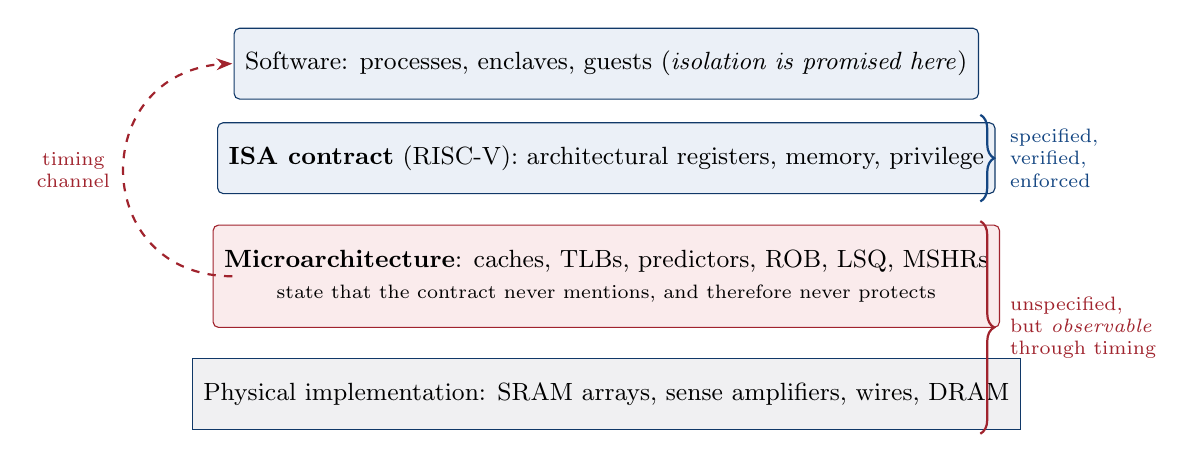
\begin{tikzpicture}[node distance=0mm]
  % Layers
  \node[blk, minimum width=9.2cm, minimum height=9mm] (sw) at (0,3.2)
        {Software: processes, enclaves, guests (\emph{isolation is promised here})};
  \node[blk, minimum width=9.2cm, minimum height=9mm, fill=lightfill] (isa) at (0,2.0)
        {\textbf{ISA contract} (RISC-V): architectural registers, memory, privilege};
  \node[atk, minimum width=9.2cm, minimum height=13mm] (ua) at (0,0.5)
        {\textbf{Microarchitecture}: caches, TLBs, predictors, ROB, LSQ, MSHRs\\
         \scriptsize state that the contract never mentions, and therefore never protects};
  \node[memblk, minimum width=9.2cm, minimum height=9mm] (phys) at (0,-1.0)
        {Physical implementation: SRAM arrays, sense amplifiers, wires, DRAM};

  % Braces / annotations
  \draw[decorate,decoration={brace,amplitude=5pt},thick,accent]
        (4.75,2.55) -- (4.75,1.45) node[midway,right=7pt,align=left,font=\scriptsize]
        {specified,\\verified,\\enforced};
  \draw[decorate,decoration={brace,amplitude=5pt},thick,attack]
        (4.75,1.2) -- (4.75,-1.5) node[midway,right=7pt,align=left,font=\scriptsize,text=attack]
        {unspecified,\\but \emph{observable}\\through timing};

  % leak arrow
  \draw[atksig] (-4.75,0.5) .. controls (-6.6,0.5) and (-6.6,3.2) .. (-4.75,3.2)
        node[midway,left=1pt,font=\scriptsize,text=attack,align=center] {timing\\channel};
\end{tikzpicture}%
}
\caption[The architecture/\uarchadj{} gap]{The gap that this paper studies.
Isolation is promised at the software level and enforced through the ISA
contract, but performance comes from state that lives \emph{below} the contract.
That state is not covered by the isolation promise, yet it is observable from
above through execution time.}
\label{fig:gap}
\end{figure}

\Cref{fig:gap} sets out the problem and fixes the vocabulary used throughout the
paper. Everything above the contract line is what a security
argument normally reasons about; everything below it is what actually determines
how long an instruction takes. The attacks in this paper are
all techniques for making information cross that line upwards.

\begin{takeaway}
The architectural state of a processor is what the ISA promises. The
\uarchadj{} state is everything else the hardware remembers so that it can be fast.
Confidentiality arguments are made about the first; attacks are mounted on the
second. A \emph{precise} exception restores architectural state exactly, and yet
leaves \uarchadj{} state modified, which is the single fact that makes
transient-execution attacks possible.
\end{takeaway}

\section{Why RISC-V specifically}
\label{sec:whyriscv}

Most of the attack literature was developed on x86 and, to a lesser extent, on
Arm. Studying the same phenomena on RISC-V is not a translation exercise\index{RISC-V!rationale for studying}; it
changes what can be said with confidence, for four reasons.

\paragraph{The specification is open and layered.} RISC-V separates a small base
integer ISA from optional extensions~\citep{riscv-unpriv}, and separates the
unprivileged ISA from the privileged architecture~\citep{riscv-priv}. This makes
it possible to say precisely which security property is a property of the
\emph{architecture} (\eg{} the \texttt{Zkt} extension's promise that certain
instructions execute in data-independent time~\citep{riscv-crypto}) and which is
a property of one \emph{implementation}. On a closed ISA that distinction is
usually unavailable to a researcher.

\paragraph{Competitive implementations are open.} Rocket (in-order,
5-stage)~\citep{asanovic2016rocket}, BOOM/SonicBOOM (superscalar
out-of-order)~\citep{zhao2020sonicboom} and CVA6/Ariane (6-stage,
Linux-capable)~\citep{zaruba2019ariane} are RTL that can be read, modified,
simulated and taped out. A claimed leak can be traced to a specific queue or
array, and a proposed defence can be implemented and measured rather than
estimated.

\paragraph{The attacks are not hypothetical here.} Spectre-style attacks have
been replicated on an open RISC-V out-of-order core and mitigations evaluated on
the same RTL~\citep{gonzalez2019replicating}, and timing-channel prevention via a
context-flush instruction has been implemented and measured on\index{CVA6 (Ariane) core}
CVA6~\citep{wistoff2021fencet}. The same openness that lets these attacks be
reproduced is what lets them be measured and fixed.

\paragraph{The defences are still being decided.} Physical memory protection
(PMP), enclave frameworks such as Sanctum~\citep{costan2016sanctum},
MI6~\citep{bourgeat2019mi6} and Keystone~\citep{lee2020keystone}, control-flow
integrity via landing pads and shadow stacks~\citep{riscv-cfi}, and proposals for
temporal partitioning are live design questions. A term paper written now can
engage with an open design space rather than describe a settled one.

\section{Prior surveys, and the origins of the field}
\label{sec:related}

The study of timing leakage is older than the term ``side channel'' as it is now
used. Kocher showed in 1996 that key-dependent execution time in
implementations of RSA and Diffie--Hellman is sufficient to recover secret
exponents~\citep{kocher1996timing}; the target there was the algorithm, not the
\uarch{}. The move to \uarchadj{} targets came with Percival's demonstration that
cache contention on a simultaneously multithreaded processor leaks across
threads~\citep{percival2005cache}, and with the AES cache-timing attacks of
Bernstein~\citep{bernstein2005aes} and of Osvik, Shamir and
Tromer~\citep{osvik2006cache}, which established the eviction and reload
primitives still in use.

Two surveys map the resulting literature. Ge \etal~\citep{ge2018survey} give a
systematic account of \uarchadj{} timing attacks and countermeasures on
contemporary hardware, organised by structure; Canella
\etal~\citep{canella2019systematic} give the corresponding systematisation for
transient-execution attacks and defences, including a classification tree that
predicted variants not then demonstrated. This paper differs from both in scope
and in intent: it is narrower, being confined to RISC-V, and it is organised
pedagogically around a single prescribed textbook rather than around the
structure of the attack space. Where a general reference on quantitative
processor design is needed beyond the prescribed text, Hennessy and
Patterson~\citep{hennessy2019quantitative} is used as a secondary source; it is
not used as a structural guideline.

\section{Research questions}
\label{sec:rqs}

The paper is organised around five questions, each answered in a specific place.

\begin{enumerate}[label=\textbf{RQ\arabic*.}, leftmargin=2.4em]
  \item \textbf{Where does the state live?} Which \uarchadj{} structures in a
        representative RISC-V pipeline retain information across a privilege or
        process boundary, and what is the granularity of that information: one bit, one cache-line address, or one branch outcome?
        (\Cref{ch:memories,ch:pipeline,ch:memsys,ch:multicore}.)
  \item \textbf{How is it read out?} What is the measurement primitive, what
        bandwidth does it achieve, and what does the attacker need to share with
        the victim: an address space, a core, a physical page, or only a socket?
        (\Cref{ch:memsys,ch:multicore,ch:transient}.)
  \item \textbf{What does speculation add?} Precisely which properties of
        speculative and out-of-order execution turn a passive side channel into
        an active one that can be steered at arbitrary victim data?
        (\Cref{ch:pipeline,ch:transient}.)
  \item \textbf{What do defences actually do?} Under a common taxonomy (partition, randomise, hide, undo, track, or forbid), what class of
        leak does each defence remove, and what does it explicitly not remove?
        (\Cref{ch:defenses}.)
  \item \textbf{What does security cost?} On a common footing of IPC, energy
        and area, what is the price of each defence class, and where does the
        Pareto frontier lie for a RISC-V core in the embedded, application and
        server classes? (\Cref{ch:tradeoffs,ch:evalplan}.)
\end{enumerate}

\section{Scope and non-goals}

\textbf{In scope.} Timing-based \uarchadj{} leakage in single-core and multicore
RISC-V processors: data and instruction caches, the TLB and page-walk hardware,
branch prediction structures, the store buffer and load-store queue, the
coherence fabric and the shared last-level cache; the transient-execution
families that use those structures as transmitters; and hardware and ISA-level
defences with their measured costs.

\textbf{Out of scope}, and deliberately so, to keep the paper coherent:
physical side channels requiring instrumentation (power analysis,
electromagnetic emanation, acoustic and optical attacks); fault-injection and
Rowhammer-style disturbance attacks~\citep{kim2014rowhammer}, which corrupt
rather than read state; cryptographic protocol weaknesses; and software-only
vulnerabilities such as memory-safety bugs, except where they interact with
speculation. Each exclusion is noted where it borders the main line of argument.

\section{Contributions of this term paper}

This is a survey-and-synthesis paper, not a paper reporting a new attack. Its
contributions are correspondingly editorial and analytical:

\begin{enumerate}[leftmargin=1.8em]
  \item \textbf{A bottom-up construction.} Rather than presenting attacks first
        and hardware afterwards, the paper builds the machine in the order of
        the prescribed textbook (ISA, memory arrays, datapath, pipeline,
        speculation, caches, virtual memory, multicore) and marks the leak at
        the moment each structure is introduced. The reader who follows the
        textbook can follow this paper in lockstep.
  \item \textbf{A RISC-V-specific evidence table} separating what has been
        \emph{demonstrated} on open RISC-V silicon or RTL from what is inferred
        by analogy with x86 (\Cref{ch:transient}).
  \item \textbf{A defence taxonomy with an explicit residual-risk column}: for
        each mechanism, what it stops, what it provably does not stop, and the
        attack that broke it if one exists, for instance speculative
        interference against invisible-speculation
        schemes~\citep{behnia2021interference}.
  \item \textbf{An explicit account of why published costs are not comparable},
        and a common-footing methodology that fixes baseline, benchmark suite and
        reporting convention so that they can be (\Cref{ch:tradeoffs}). In v0.1
        the cost columns are qualitative and every figure derived from them is
        labelled as illustrative; populating them with numbers measured on one
        platform is the object of \Cref{ch:evalplan}.
  \item \textbf{A concrete, executable evaluation plan} for the author's own
        measurements on an open RISC-V core (\Cref{ch:evalplan}), which versions
        v0.2 and v0.3 will carry out.
\end{enumerate}

\section{Mapping to the prescribed textbook's Table of Contents}
\label{sec:tocmap}

The Table of Contents of the prescribed textbook, S.~R.~Sarangi, \textit{Basic
Computer Architecture}~\citep{sarangi2025basic}, is used as the structural
guideline for this paper. \Cref{fig:roadmap} shows the correspondence
graphically and \Cref{tab:tocmap} gives it at chapter and section granularity;
\Cref{app:tocmap} expands it to sub-section granularity with a sentence on the
role each sub-section plays.

\textbf{Primary chapters} (the spine of the paper): Chapters~6, 9, 10, 11
and~12. \textbf{Supporting chapters} (added for completeness of the argument):
Chapters~1 and~7. No other textbook is used as a structural guideline; all other
sources are research papers and specifications used as evidence, not as skeleton.

\begin{figure}[t]
\centering
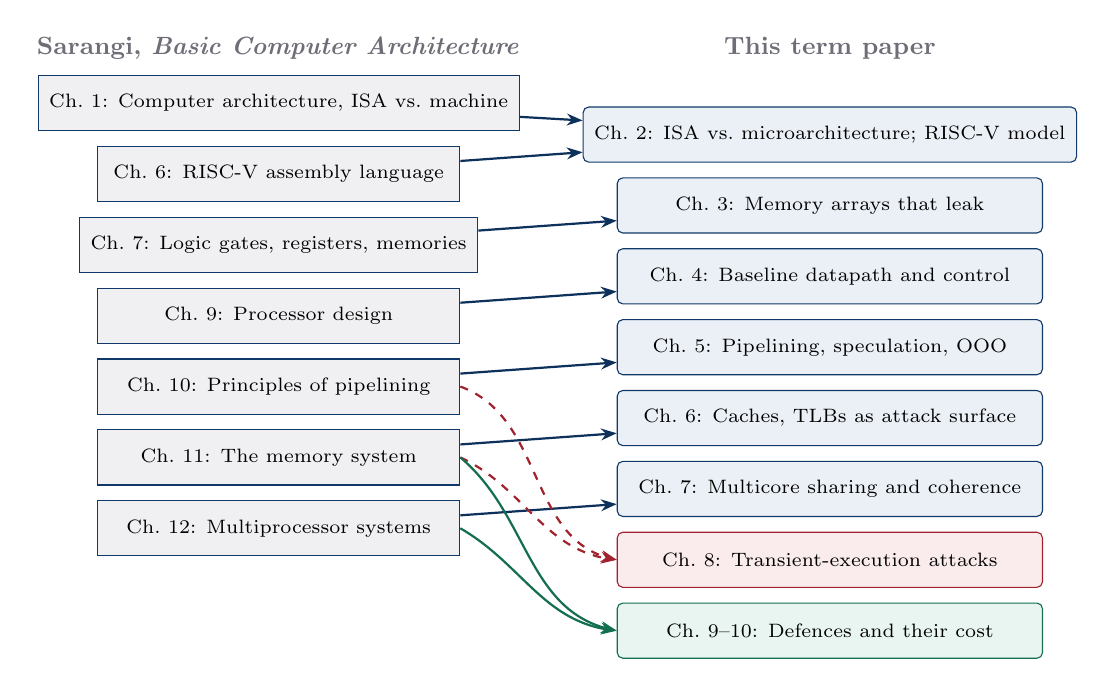
\begin{tikzpicture}[node distance=2mm]
  \tikzset{tb/.style={memblk, minimum width=4.6cm, font=\scriptsize, minimum height=7mm},
           pp/.style={blk, minimum width=5.4cm, font=\scriptsize, minimum height=7mm}}
  % textbook column
  \node[font=\small\bfseries, text=muted] at (-3.4,1.1) {Sarangi, \textit{Basic Computer Architecture}};
  \node[tb] (t1)  at (-3.4, 0.4) {Ch.~1: Computer architecture, ISA vs.\ machine};
  \node[tb] (t6)  at (-3.4,-0.5) {Ch.~6: RISC-V assembly language};
  \node[tb] (t7)  at (-3.4,-1.4) {Ch.~7: Logic gates, registers, memories};
  \node[tb] (t9)  at (-3.4,-2.3) {Ch.~9: Processor design};
  \node[tb] (t10) at (-3.4,-3.2) {Ch.~10: Principles of pipelining};
  \node[tb] (t11) at (-3.4,-4.1) {Ch.~11: The memory system};
  \node[tb] (t12) at (-3.4,-5.0) {Ch.~12: Multiprocessor systems};

  % paper column
  \node[font=\small\bfseries, text=muted] at (3.6,1.1) {This term paper};
  \node[pp] (p2)  at (3.6, 0.0) {Ch.~2: ISA vs.\ \uarch{}; RISC-V model};
  \node[pp] (p3)  at (3.6,-0.9) {Ch.~3: Memory arrays that leak};
  \node[pp] (p4)  at (3.6,-1.8) {Ch.~4: Baseline datapath and control};
  \node[pp] (p5)  at (3.6,-2.7) {Ch.~5: Pipelining, speculation, OOO};
  \node[pp] (p6)  at (3.6,-3.6) {Ch.~6: Caches, TLBs as attack surface};
  \node[pp] (p7)  at (3.6,-4.5) {Ch.~7: Multicore sharing and coherence};
  \node[pp, fill=attackfill, draw=attack] (p8) at (3.6,-5.4) {Ch.~8: Transient-execution attacks};
  \node[pp, fill=defensefill, draw=defense] (p9) at (3.6,-6.3) {Ch.~9--10: Defences and their cost};

  \draw[sig] (t1)  -- (p2);
  \draw[sig] (t6)  -- (p2);
  \draw[sig] (t7)  -- (p3);
  \draw[sig] (t9)  -- (p4);
  \draw[sig] (t10) -- (p5);
  \draw[sig] (t11) -- (p6);
  \draw[sig] (t12) -- (p7);
  \draw[atksig] (t10.east) to[out=-20,in=170] (p8.west);
  \draw[atksig] (t11.east) to[out=-25,in=175] (p8.west);
  \draw[defsig] (t11.east) to[out=-40,in=170] (p9.west);
  \draw[defsig] (t12.east) to[out=-30,in=175] (p9.west);
\end{tikzpicture}
\caption[Textbook-to-paper chapter mapping]{Correspondence between the
prescribed textbook's chapters and the chapters of this paper. Solid arrows
carry background material; dashed red and solid green arrows show where two
textbook chapters (pipelining and the memory system) jointly support the attack
and defence chapters, which have no direct textbook counterpart.}
\label{fig:roadmap}
\end{figure}

\begin{table}[p]
\centering
\caption[Chapter- and section-level textbook mapping]{Chapter- and section-level
mapping between the prescribed textbook~\citep{sarangi2025basic} and this paper.
``Primary'' marks the five chapters that form the spine of the term paper.
Sub-section granularity is given in \Cref{app:tocmap}.}
\label{tab:tocmap}
\footnotesize
\begin{tabularx}{\linewidth}{@{}p{1.6cm}p{2.6cm}p{1.6cm}X@{}}
\toprule
\textbf{Textbook} & \textbf{Sections used} & \textbf{Role} & \textbf{How it is used in this paper} \\
\midrule
Ch.~1 & 1.4, 1.5, 1.7 & Supporting &
The architecture-versus-organization definitions that open the chapter, the
language of instructions, instruction set design, and the design of practical
machines. Used in \Cref{ch:isa} to argue that an open, well-defined
ISA constrains \emph{results} and therefore cannot by itself prevent
implementation-level leakage. \\
\addlinespace
Ch.~6 & 6.1.1--6.1.2, 6.3.1--6.3.3, 6.5 & \textbf{Primary} &
RISC-V base ISAs and extensions; the register view; conditional and
unconditional control transfer; load/store instructions; instruction encoding.
Used in \Cref{ch:isa} for the execution model, for the branch and memory
instructions that drive predictors and caches, and for the encoding space in
which security instructions (barriers, flushes) must be placed. \\
\addlinespace
Ch.~7 & 7.4 (7.4.1--7.4.3) & Supporting &
Memories: static RAM and its arrays, content-addressable memory, and dynamic
RAM. Used in
\Cref{ch:memories} as the physical explanation of why cache, TLB and predictor
accesses have data-dependent latency at all. \\
\addlinespace
Ch.~9 & 9.1, 9.2 (9.2.1--9.2.7), 9.3 & \textbf{Primary} &
Baseline processor: the fetch unit, data path and control path, operand fetch,
execute, memory access, register writeback, the assembled data path, and the
control unit. Used in \Cref{ch:proc} to fix the
reference machine onto which predictors, buffers and caches are later added. \\
\addlinespace
Ch.~10 & 10.1--10.4, 10.8 (10.8.2, 10.8.3), 10.9.3, 10.10 (10.10.2, 10.10.5), 10.11 (10.11.1, 10.11.4) & \textbf{Primary} &
Pipelining; data, control and structural hazards; exceptions and \emph{precise}
exceptions; performance of a non-ideal pipeline; power, dynamic power and the
$ED^{2}$ metric; branch prediction and out-of-order pipelines.
Used in \Cref{ch:pipeline} for speculation and the execution window, in
\Cref{ch:transient} for why precise exceptions do not undo \uarchadj{} effects, and
in \Cref{ch:tradeoffs} for the IPC, power and energy metrics used to price
defences. \\
\addlinespace
Ch.~11 & 11.1.2--11.1.8, 11.2, 11.3 (11.3.1), 11.4 (11.4.2, 11.4.3, 11.4.5, 11.4.6) & \textbf{Primary} &
Locality and the memory hierarchy; caches, their lookup, insertion, replacement
and eviction; the mathematical model of the memory system; virtual memory,
paging, the memory management unit and advanced paging features. Used in \Cref{ch:memsys} for every cache and TLB attack
primitive and for the AMAT-based cost model of flushing and partitioning. \\
\addlinespace
Ch.~12 & 12.2, 12.3, 12.4 (12.4.1--12.4.6, 12.4.8) & \textbf{Primary} &
Software for multiprocessors and Amdahl's law; the multiprocessor design space;
coherence, memory consistency, the physical view of memory, shared caches,
coherent private caches and multithreaded processors. Used in
\Cref{ch:multicore} for cross-core and cross-thread leakage. Cache partitioning
and colouring, used there as \emph{defences}, are not textbook material and are
drawn from the research literature instead. \\
\bottomrule
\end{tabularx}
\end{table}

\begin{tocmapbox}
Throughout the paper, a box like this one appears at the start of a section to
name the exact textbook section that supplies the background for what follows.
This keeps the correspondence in \Cref{tab:tocmap} verifiable at the point of
use, rather than only in the front matter.
\end{tocmapbox}

\section{Organisation of the report}

\Cref{ch:isa} establishes the ISA/\uarchadj{} distinction and the RISC-V execution
model, and states the threat model used for the rest of the paper.
\Cref{ch:memories} descends to the memory arrays. \Cref{ch:proc} builds the
baseline datapath and \Cref{ch:pipeline} pipelines it and adds branch prediction
and out-of-order execution; the performance and power metrics it points to are
defined in \Cref{app:metrics}.
\Cref{ch:memsys} treats the cache hierarchy and virtual memory as an attack
surface, and \Cref{ch:multicore} extends this to multicore sharing and coherence.
\Cref{ch:transient} synthesises the transient-execution families.
\Cref{ch:defenses} builds the defence taxonomy and \Cref{ch:tradeoffs} prices
it. \Cref{ch:evalplan} specifies the author's own evaluation, and
\Cref{ch:conclusion} concludes.

Six appendices follow. \Cref{app:plagiarism} is the plagiarism report and
\Cref{app:readability} the reading indices for this text.
\Cref{app:metrics} holds the cost-metric definitions that \Cref{ch:tradeoffs}
prices defences with. \Cref{app:tocmap} gives the fine-grained textbook mapping,
\Cref{app:toolchain} documents the toolchain and the single-file build, and
\Cref{app:changelog} is the change log and the plan for v0.2 and v0.3. A
Glossary, an Index, a List of Tables, a List of Figures and a List of Listings
are generated automatically.

\section{Status of this draft}
\label{sec:status}

\begin{draftnote}
\textbf{What v0.1 contains:} the full structure; the textbook mapping at
chapter, section and sub-section granularity; the threat model; developed
technical text in all twelve chapters; the complete figure programme (every
figure drawn programmatically, none imported); the defence taxonomy and the cost
tables in first-pass form; and the bibliography.

\textbf{What v0.1 does not yet contain, by design:}
(i) the author's own measurements: every quantitative figure currently
carries a citation to its original source and is labelled as such;
(ii) the formal leakage model of \Cref{sec:leakmodel}, currently stated
informally;
(iii) the full RTL walk-through of a RISC-V load path, planned for v0.2;
(iv) roughly two-fifths of the target word count.
\Cref{app:changelog} lists each item with its target version.
\end{draftnote}

\chapter{The Contract and the Machine: RISC-V as Architecture and as Implementation}
\label{ch:isa}

\begin{tocmapbox}
Background: textbook Chapter~1 (which defines \emph{architecture} as the view of
a computer presented to software designers and \emph{organization} as its actual
hardware implementation), \SecRef{1.4} (the language of instructions),
\SecRef{1.5} (instruction set design) and \SecRef{1.7} (design of practical
machines);
\SecRef{6.1.1} (RISC-V base ISAs and extensions), \SecRef{6.1.2} (view of
registers), \SecRef{6.3.1}--\SecRef{6.3.3} (branches and memory instructions),
\SecRef{6.5} (instruction encoding)~\citep{sarangi2025basic}.
\end{tocmapbox}

\section{An ISA is a contract about values, not about time}
\label{sec:contract}

The textbook draws the distinction that the whole of this paper depends on, in
the opening definition of Chapter~1: the \emph{architecture} is the view of a
computer presented to software designers, while the \emph{organization} is the
actual implementation of that computer in hardware. Two implementations of the same ISA must agree on the value
written into every architectural register and every memory location; they need
not agree on anything else, and in practice they do not agree on almost
everything else: pipeline depth, issue width, cache sizes, predictor
organisation, replacement policy.

Write the contract explicitly. Let $A$ be the architectural state: the general
purpose registers, the program counter, the control and status registers visible\index{architectural state}
at the current privilege level, and memory. Let $\mu$ be the \uarchadj{} state:
cache contents and their replacement metadata, TLB entries, branch history and\index{microarchitectural state}
target tables, the reorder buffer, the load-store queue, miss-status holding
registers, line-fill and store buffers, prefetcher tables. An implementation is
\emph{architecturally correct} if, for every program $P$ and initial
architectural state $A_0$,
\begin{equation}
  \mathrm{exec}(P, A_0) \;=\; A_n
  \label{eq:contract}
\end{equation}
where $A_n$ is the architecturally specified final state. \Cref{eq:contract}
quantifies over nothing at all in $\mu$, and it says nothing about the number of
cycles taken. The contract is therefore satisfied by an implementation whose
$\mu$ depends arbitrarily on secret data, and whose execution time depends
arbitrarily on $\mu$. Composing those two dependences gives a channel from
secret data to execution time.

\begin{takeaway}
Every attack in this paper is an instance of one pattern: find a computation
whose effect on $\mu$ depends on a secret, and find a way to convert $\mu$ back
into time. The ISA is not violated at any point, so ISA-level reasoning cannot
close these channels by itself, however open and however precise the
specification.
\end{takeaway}

An open ISA does not change \Cref{eq:contract}; it changes who can inspect the
implementation. That is the argument for studying RISC-V made in \Cref{sec:whyriscv}: openness helps the analyst, not the attacker, because the
attacker never needed the specification, only a stopwatch.

\section{The RISC-V execution model}

\subsection{Base ISAs and extensions}

RISC-V is defined as a small base integer instruction set plus optional standard
extensions~\citep{riscv-unpriv}. The base is RV32I or RV64I (and the reduced\index{RISC-V!base integer ISA}
RV32E for embedded cores); extensions add multiplication and division (M),
atomics (A), floating point (F, D, Q), compressed 16-bit encodings (C), vectors\index{RISC-V!standard extensions}
(V), bit manipulation (B), and cryptography (K). The conventional shorthand
\texttt{RV64GC} denotes RV64IMAFDC.

This modularity matters for security in a way that is easy to miss. Each
extension is a set of promises about \emph{results}; only a handful of
extensions make any promise about \emph{timing}. \Cref{tab:extensions} lists the
extensions and architectural features that bear directly on the subject of this
paper, and states what each does and does not promise.

\begin{table}[t]
\centering
\caption[RISC-V features relevant to \uarchadj{} security]{RISC-V architectural
features that bear on \uarchadj{} security, and the limits of what each guarantees.
The right-hand column is the one that matters: most of these features constrain
\emph{results} or \emph{access rights}, not \emph{timing}.}
\label{tab:extensions}
\footnotesize
\begin{tabularx}{\linewidth}{@{}p{2.5cm}p{3.5cm}X@{}}
\toprule
\textbf{Feature} & \textbf{What it provides} & \textbf{What it does \emph{not} provide} \\
\midrule
PMP / ePMP \newline (privileged arch.) &
Physical-address-range access control checked by M-mode~\citep{riscv-priv}. &
No control over whether a denied access has already perturbed a cache or a
predictor; PMP is an architectural check, not a \uarchadj{} one. \\
\addlinespace
Sv39 / Sv48 paging &
Virtual memory, per-page permissions, ASIDs~\citep{riscv-priv}. &
Nothing about TLB residency, page-walk caching, or the timing of a walk, which is the substrate for TLB attacks~\citep{gras2018tlbleed}. \\
\addlinespace
\texttt{Zkt} &
An architectural promise that a listed set of instructions executes in time
independent of their data operands~\citep{riscv-crypto}. &
Only covers the listed instructions and only data-operand independence; says
nothing about \emph{address}-dependent timing, which is what caches leak. \\
\addlinespace
\texttt{Zicfilp}, \texttt{Zicfiss} &
Landing pads and a shadow stack for control-flow integrity~\citep{riscv-cfi}. &
CFI constrains architectural control flow; speculative control flow can still be
steered, so CFI is not a Spectre-v2 defence by itself. \\
\addlinespace
\texttt{fence}, \texttt{fence.i}, \texttt{sfence.vma} &
Ordering of memory and instruction-fetch, TLB invalidation. &
Ordering is not erasure: a \texttt{fence} does not remove the cache lines or
predictor entries installed before it. \\
\addlinespace
\texttt{fence.t} \newline (proposed) &
Temporal fence: flush \uarchadj{} state at a context switch and normalise
timing~\citep{wistoff2021fencet}. &
Not yet standard; cost grows with the amount of state flushed
(\Cref{ch:tradeoffs}). \\
\addlinespace
\texttt{cbo.flush}, \texttt{cbo.inval} (Zicbom) &
Architectural cache-block management. &
A double-edged feature: block flushing by address is also the primitive that
makes Flush+Reload possible~\citep{yarom2014flushreload}. \\
\bottomrule
\end{tabularx}
\end{table}

The last row deserves emphasis. Cache-management instructions were added for
correctness with non-coherent DMA and for performance, and they are genuinely
useful. They also hand an attacker a precise, architecturally sanctioned way to\index{cache management instructions (Zicbom)}
evict a chosen line, which is the primitive Flush+Reload requires\index{Flush+Reload}. The
same instruction is a feature at one layer and a transmitter at another. This
tension (performance and manageability features that double as attack
primitives) recurs throughout the paper.

\subsection{Register view and the shape of a computation}

RV64I provides 32 general purpose registers \code{x0}--\code{x31}, with
\code{x0} hardwired to zero, plus the program counter. The application binary
interface assigns roles (\code{ra} for the return address, \code{sp} for the
stack pointer, \code{a0}--\code{a7} for arguments, \code{t}$n$ and \code{s}$n$
for temporaries and saved registers). Registers are architectural state: on a
context switch the operating system saves and restores them, and after the
restore the new context cannot tell what the old context held.

That property is what makes the contrast with \uarchadj{} state so sharp. There is
no instruction that saves and restores the branch history register, and no\index{context switch!predictor state not scrubbed}
requirement that a context switch clear it. The register file is scrubbed; the
predictor is not. The attacks of \Cref{ch:transient} all turn on asymmetries of this
kind.

\subsection{Control transfer and memory instructions}
\label{sec:ctrlmem}

Two instruction classes drive every structure this paper is concerned with.

\textbf{Conditional branches} (B-type: \code{beq}, \code{bne}, \code{blt},
\code{bge}, \code{bltu}, \code{bgeu}) compare two registers and add a
sign-extended immediate to the PC. \textbf{Unconditional transfers} are
\code{jal} (PC-relative, writes the return address) and \code{jalr} (register
indirect, the basis of returns and indirect calls). Branch outcomes train the
direction predictor; \code{jalr} targets train the branch target buffer and the\index{branch target buffer (BTB)}
return-address stack. Every one of these structures is shared, and none is\index{return address stack (RAS)}
architecturally scrubbed.

\textbf{Loads and stores} (\code{lb}, \code{lh}, \code{lw}, \code{ld} and their
unsigned variants; \code{sb}, \code{sh}, \code{sw}, \code{sd}) compute an
effective address as a base register plus a sign-extended 12-bit immediate.\index{load and store instructions!effective address}
Two things follow. First, the address is \emph{data-dependent} whenever the base
register holds a value derived from data, which is the case in every table
lookup, and in particular in an S-box lookup. Second, the latency of the access
depends on where the line is found. Put those two facts together and you have the
cache side channel.

\begin{lstlisting}[language=riscv, caption={The canonical leak, in RISC-V. The
address of the second load depends on a secret byte; its latency therefore
reveals which line was touched. Nothing here violates the ISA.},
label={lst:leak}]
# a0 = pointer to secret byte, a1 = base of a 256*64-byte probe array
  lbu   t0, 0(a0)        # t0 = secret byte  (0..255)
  slli  t0, t0, 6        # t0 = secret * 64  (one cache line per value)
  add   t1, a1, t0       # address depends on the secret
  lbu   t2, 0(t1)        # this access installs ONE line of the probe array
# ...the value in t2 is never used; the *state change* is the message.
\end{lstlisting}

\Cref{lst:leak} is the transmitter used, with minor variations, by every attack
in \Cref{ch:transient}. Note what it does not do: it does not write the secret
anywhere architecturally visible, and if the sequence is later squashed the
architectural effect is nil. The line installed by the last load, however,
remains.

\subsection{Instruction encoding and the room for security instructions}

\Cref{fig:encoding} shows the six base instruction formats. The encoding is
deliberately regular: source register fields sit at fixed positions in every\index{RISC-V!instruction encoding}
format so that register-file reads can begin before decoding
completes~\citep{riscv-unpriv}. It is a small but real example of the textbook theme of \SecRef{1.7}: the
practical machine shapes the specification.

\begin{figure}[t]
\centering
\resizebox{\linewidth}{!}{%
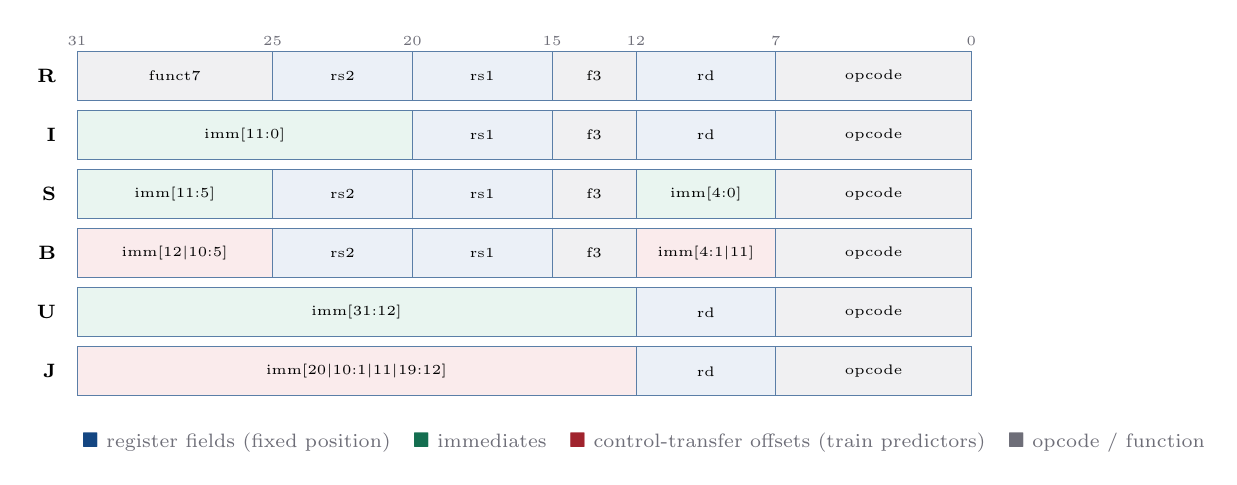
\begin{tikzpicture}[x=3.55mm, y=1cm]
  \newcommand{\fld}[5]{%
    \draw[fill=#5, draw=accent!70, line width=0.3pt] (#1,#2) rectangle ++(#3,0.62);
    \node[font=\tiny] at ({#1+#3/2}, {#2+0.31}) {#4};}
  % bit ruler
  \foreach \b/\x in {31/0, 25/7, 20/12, 15/17, 12/20, 7/25, 0/32}
     {\node[font=\tiny, text=muted] at (\x,4.85) {\b};}
  % R-type  (y=4.1)
  \node[font=\scriptsize\bfseries, anchor=east] at (-0.4,4.41) {R};
  \fld{0}{4.1}{7}{funct7}{greyfill}\fld{7}{4.1}{5}{rs2}{lightfill}
  \fld{12}{4.1}{5}{rs1}{lightfill}\fld{17}{4.1}{3}{f3}{greyfill}
  \fld{20}{4.1}{5}{rd}{lightfill}\fld{25}{4.1}{7}{opcode}{greyfill}
  % I-type (y=3.35)
  \node[font=\scriptsize\bfseries, anchor=east] at (-0.4,3.66) {I};
  \fld{0}{3.35}{12}{imm[11:0]}{defensefill}\fld{12}{3.35}{5}{rs1}{lightfill}
  \fld{17}{3.35}{3}{f3}{greyfill}\fld{20}{3.35}{5}{rd}{lightfill}
  \fld{25}{3.35}{7}{opcode}{greyfill}
  % S-type (y=2.6)
  \node[font=\scriptsize\bfseries, anchor=east] at (-0.4,2.91) {S};
  \fld{0}{2.6}{7}{imm[11:5]}{defensefill}\fld{7}{2.6}{5}{rs2}{lightfill}
  \fld{12}{2.6}{5}{rs1}{lightfill}\fld{17}{2.6}{3}{f3}{greyfill}
  \fld{20}{2.6}{5}{imm[4:0]}{defensefill}\fld{25}{2.6}{7}{opcode}{greyfill}
  % B-type (y=1.85)
  \node[font=\scriptsize\bfseries, anchor=east] at (-0.4,2.16) {B};
  \fld{0}{1.85}{7}{imm[12$|$10:5]}{attackfill}\fld{7}{1.85}{5}{rs2}{lightfill}
  \fld{12}{1.85}{5}{rs1}{lightfill}\fld{17}{1.85}{3}{f3}{greyfill}
  \fld{20}{1.85}{5}{imm[4:1$|$11]}{attackfill}\fld{25}{1.85}{7}{opcode}{greyfill}
  % U-type (y=1.1)
  \node[font=\scriptsize\bfseries, anchor=east] at (-0.4,1.41) {U};
  \fld{0}{1.1}{20}{imm[31:12]}{defensefill}\fld{20}{1.1}{5}{rd}{lightfill}
  \fld{25}{1.1}{7}{opcode}{greyfill}
  % J-type (y=0.35)
  \node[font=\scriptsize\bfseries, anchor=east] at (-0.4,0.66) {J};
  \fld{0}{0.35}{20}{imm[20$|$10:1$|$11$|$19:12]}{attackfill}\fld{20}{0.35}{5}{rd}{lightfill}
  \fld{25}{0.35}{7}{opcode}{greyfill}
  % legend
  \node[note, anchor=west] at (0,-0.25)
    {\textcolor{accent}{$\blacksquare$}~register fields (fixed position)\quad
     \textcolor{defense}{$\blacksquare$}~immediates\quad
     \textcolor{attack}{$\blacksquare$}~control-transfer offsets (train predictors)\quad
     $\blacksquare$~opcode / function};
\end{tikzpicture}%
}
\caption[RISC-V base instruction formats]{The six base RISC-V instruction
formats, drawn to bit scale (textbook \SecRef{6.5}). The \code{rs1}, \code{rs2}
and \code{rd} fields occupy the same bit positions in every format, so the
register file can be read speculatively during decode, a \uarch{}
optimisation visible in the architecture. The B- and J-type offsets (red) are
what train the direction predictor, the branch target buffer and the
return-address stack; the I- and S-type immediates feed effective-address
computation and therefore the cache.}
\label{fig:encoding}
\end{figure}

The encoding also determines where a security feature can go. Adding a fence
that flushes \uarchadj{} state, \code{fence.t} in the proposal of Wistoff
\etal~\citep{wistoff2021fencet}, means consuming encoding space in the
\texttt{MISC-MEM} opcode, and adding CSRs to configure it. Encoding space is
finite and contested; a defence that needs a new instruction competes with
performance extensions for it. It is one reason many hardware defences in \Cref{ch:defenses} are designed to
be \emph{transparent}, requiring no ISA
change at all, even at the cost of being harder to reason about.

\section{Architectural versus microarchitectural state, precisely}
\label{sec:archvsuarch}

\Cref{tab:statepartition} partitions the state of a representative RISC-V core.
The classification criterion is operational: state is architectural if a correct
implementation is obliged to restore it on an exception or a context switch, and
\uarch{} if it is not.

\begin{table}[t]
\centering
\caption[Partition of processor state]{Partition of the state of a
representative out-of-order RISC-V core. The final column gives the observation
granularity (how much an attacker learns from one successful measurement of
that structure), which is the quantity that determines channel bandwidth in
\Cref{ch:memsys}.}
\label{tab:statepartition}
\footnotesize
\begin{tabularx}{\linewidth}{@{}p{2.75cm}p{2.55cm}X p{2.2cm}@{}}
\toprule
\textbf{Structure} & \textbf{Class} & \textbf{Scrubbed on context switch?} & \textbf{Granularity} \\
\midrule
\code{x0}--\code{x31}, PC, CSRs & Architectural & Yes, by the OS & not a channel \\
Memory, page tables            & Architectural & Protected by PMP/paging & not a channel \\
\midrule
L1D / L1I / L2 / LLC data arrays & \Uarch{} & No (unless flushed explicitly) & Cache line (\SI{64}{\byte}) \\
Cache replacement metadata       & \Uarch{} & No & Way within a set \\
TLB, page-walk caches            & \Uarch{} & Partially (ASID-tagged) & Page (\SI{4}{\kibi\byte}) \\
Branch direction predictor       & \Uarch{} & No & 1 bit per branch \\
Branch target buffer             & \Uarch{} & No & Target address bits \\
Return address stack             & \Uarch{} & No & Call depth and target \\
Reorder buffer, issue queues     & \Uarch{} & Drained, not cleared & Occupancy / timing \\
Store buffer, load-store queue   & \Uarch{} & Drained & Address match (STL forwarding) \\
MSHRs, line-fill buffers         & \Uarch{} & No & In-flight line identity \\
Prefetcher stream tables         & \Uarch{} & No & Access stride \\
DRAM row buffers (\SecRef{7.4.3}) & \Uarch{} & No & DRAM row \\
\bottomrule
\end{tabularx}
\end{table}

Two rows of \Cref{tab:statepartition} deserve a second look. The reorder buffer is
``drained, not cleared'': its \emph{contents} do not survive, but its
\emph{occupancy} affects the timing of subsequent instructions, and contention
for it is measurable. And the TLB is only ``partially'' scrubbed: ASID
tagging avoids the need to flush, which is a performance win that leaves entries\index{address-space identifier (ASID)}
from other address spaces resident and therefore contendable.

\section{Threat model}
\label{sec:threat}

A leakage claim is meaningless without saying who the attacker is.\index{threat model} This paper
uses the four-tier model of \Cref{tab:threat} throughout; every attack discussed
later is labelled with the weakest tier at which it works.

\begin{table}[t]
\centering
\caption[Threat model tiers]{Threat model. Tiers are ordered by decreasing
attacker capability. Each attack in \Cref{ch:memsys,ch:multicore,ch:transient} is
annotated with the weakest tier at which it has been demonstrated.}
\label{tab:threat}
\footnotesize
\begin{tabularx}{\linewidth}{@{}p{1.2cm}p{3.4cm}X@{}}
\toprule
\textbf{Tier} & \textbf{Attacker position} & \textbf{Capabilities assumed} \\
\midrule
T1 & Same address space \newline (sandboxed code) &
Runs attacker-chosen code in the victim's address space (JIT-compiled script, eBPF
program, plugin). Can time its own instructions. Cannot read victim memory
architecturally. This is the Spectre-v1 setting. \\
\addlinespace
T2 & Same core, different process or privilege level &
Time-shares a core with the victim; shares L1, TLB and all predictors across the
context switch. Requires only an ordinary unprivileged process. \\
\addlinespace
T3 & Different core, same package &
Shares only the last-level cache, the interconnect, the memory controller and
DRAM. The realistic cloud co-tenancy setting~\citep{liu2015llc}. \\
\addlinespace
T4 & Remote &
Observes only end-to-end response times over a network. Low bandwidth, high
noise, but no local code execution required. \\
\bottomrule
\end{tabularx}
\end{table}

\textbf{Assumptions common to all tiers.} The attacker knows the \uarch{} in
detail, an assumption that is trivially satisfied for open RISC-V cores and
approximately satisfied for closed ones through reverse engineering. The
attacker has access to a timing source: \code{rdcycle} or \code{rdtime} where
permitted, a counting thread otherwise; restricting timer resolution raises cost
but does not close channels. The attacker cannot mount physical attacks, cannot
induce faults, and cannot exploit software memory-safety bugs (those are out of
scope, \Cref{ch:intro}). Cryptography is assumed correct, so that any key
recovery discussed is attributable to the \uarch{}, not to the algorithm.

\section{Towards a leakage model}
\label{sec:leakmodel}

Informally, a channel exists when there is a function from secret bits to\index{leakage model}
observable time. Writing $\mathcal{O}$ for the attacker's observation (a vector
of measured latencies) and $s$ for the secret, a channel exists when
$I(s;\mathcal{O}) > 0$, and its capacity bounds the attack's bandwidth. The
practical questions (how many measurements are needed, how noise reduces the
rate, how error-correcting repetition trades bandwidth for reliability) are
information-theoretic, and \Cref{ch:memsys} treats the cache case quantitatively.

\begin{draftnote}
This section is intentionally short in v0.1. For v0.2 it will be developed into a
formal treatment: (a) definition of an observation function over $\mu$;
(b) the standard channel-capacity bound for a binary asymmetric channel modelling
a hit/miss observation with measurement noise; (c) a worked estimate of achievable
bits/second for Prime+Probe on an L1 of a given associativity, cross-checked
against the rates reported by Yarom and Falkner~\citep{yarom2014flushreload} and
Liu \etal~\citep{liu2015llc}; and (d) a discussion of why constant-time
programming disciplines amount to requiring that this function be constant
in $s$. Target length: 3--4 pages.
\end{draftnote}

\chapter{The Physical Substrate: Memory Arrays That Remember Too Much}
\label{ch:memories}

\begin{tocmapbox}
Background: textbook \SecRef{7.4} (memories) and its sub-sections
\SecRef{7.4.1} (static RAM), \SecRef{7.4.2} (content-addressable memory) and
\SecRef{7.4.3} (dynamic RAM)~\citep{sarangi2025basic}.
\end{tocmapbox}

\section{Why a security paper has to go down to the array}

It is possible to describe cache attacks purely at the level of hits and misses,
and most surveys do. The cost of that abstraction is that two important facts
become mysterious: \emph{why} a hit and a miss differ by tens of nanoseconds
rather than by a few picoseconds, and \emph{why} the difference is stable enough
to measure reliably from software. Both answers live in the array. This chapter
therefore spends a few pages at the transistor and array level, and then never
returns there, but the rest of the paper rests on it.

\section{The storage cell}

\Cref{fig:sram} shows the standard six-transistor SRAM cell: two cross-coupled\index{SRAM!six-transistor cell}
inverters holding a bit, and two access transistors connecting the internal
nodes $Q$ and $\overline{Q}$ to a pair of bit lines when the word line is
asserted.

\begin{figure}[t]
\centering
\begin{circuitikz}[scale=0.95, transform shape]
  % --- storage core: two cross-coupled inverters -------------------
  \draw (0,0.75)  node[not port](I1){};
  \draw (0,-0.75) node[not port, rotate=180](I2){};
  \draw (I1.out) -- (1.1,0.75) -- (1.1,-0.75) -- (I2.in);
  \draw (I2.out) -- (-1.1,-0.75) -- (-1.1,0.75) -- (I1.in);
  \node[font=\scriptsize, right] at (1.15,0.15) {$\overline{Q}$};
  \node[font=\scriptsize, left]  at (-1.15,0.15) {$Q$};

  % --- access transistors ------------------------------------------
  \draw (-2.0,0) node[nmos, rotate=-90](AL){};
  \draw ( 2.0,0) node[nmos, rotate=-90](AR){};
  \draw (AL.drain) -- (-1.1,0);   \filldraw (-1.1,0) circle (1.3pt);
  \draw (AR.source) -- (1.1,0);   \filldraw ( 1.1,0) circle (1.3pt);
  \draw (AL.source) -- (-3.0,0);
  \draw (AR.drain)  -- ( 3.0,0);

  % --- word line ----------------------------------------------------
  \draw[accent, thick] (-3.6,1.9) -- (3.6,1.9)
        node[right, font=\scriptsize, black] {WL};
  \draw (AL.gate) -- (-2.0,1.9); \filldraw (-2.0,1.9) circle (1.3pt);
  \draw (AR.gate) -- ( 2.0,1.9); \filldraw ( 2.0,1.9) circle (1.3pt);

  % --- bit lines ----------------------------------------------------
  \draw[accent, thick] (-3.0,-2.3) -- (-3.0,2.7) node[above, font=\scriptsize, black] {BL};
  \draw[accent, thick] ( 3.0,-2.3) -- ( 3.0,2.7) node[above, font=\scriptsize, black] {$\overline{\text{BL}}$};

  % --- precharge and sense amp blocks -------------------------------
  \node[memblk, font=\scriptsize, minimum width=2.4cm, minimum height=6mm] (pc) at (0,2.7)
        {precharge / equalise};
  \draw (pc.west) -- (-3.0,2.7);  \draw (pc.east) -- (3.0,2.7);
  \node[memblk, font=\scriptsize, minimum width=2.4cm, minimum height=6mm] (sa) at (0,-2.3)
        {sense amplifier};
  \draw (sa.west) -- (-3.0,-2.3); \draw (sa.east) -- (3.0,-2.3);
  \draw[sig] (sa.south) -- ++(0,-0.6) node[below, font=\scriptsize] {data out};

  % --- annotations ---------------------------------------------------
  \node[note, anchor=west, text width=4.1cm] at (3.9,0.4)
        {The cell can only pull the bit lines apart slowly: it is sized to be
         \emph{small}, not strong. The delay from WL rising to a resolvable
         $\Delta V$ is the irreducible core of access latency.};
\end{circuitikz}
\caption[Six-transistor SRAM cell]{The 6T SRAM cell (textbook \SecRef{7.4.1}).
Two cross-coupled inverters store the bit; two access transistors couple it to a
precharged differential bit-line pair when the word line is asserted. Reading is
destructive-by-degree: the cell must discharge a large bit-line capacitance
through a deliberately weak transistor, which is why an array access costs
hundreds of picoseconds to nanoseconds rather than a gate delay.}
\label{fig:sram}
\end{figure}

Two design pressures shape the cell, and both have security consequences. The
cell is made as small as possible, so its transistors are weak and the bit-line
swing develops slowly; a sense amplifier is therefore needed, and sensing has to
be timed. And bit lines are shared down a whole column, so their capacitance is
large and the array is organised into banks and sub-arrays to keep the shared
wire short. The result is a structure whose access time is a real, measurable
quantity of the order of a clock cycle for a small array and many cycles for a
large one, a difference that software can time.

\section{From cell to array}

\Cref{fig:array} shows the organisation described in \SecRef{7.4.1}: a decoder converts an
address into one asserted word line, a two-dimensional cell array holds the data,
sense amplifiers convert small differential voltages into logic levels, and a
column multiplexer selects the required subset of bits.

\begin{figure}[t]
\centering
\resizebox{\linewidth}{!}{%
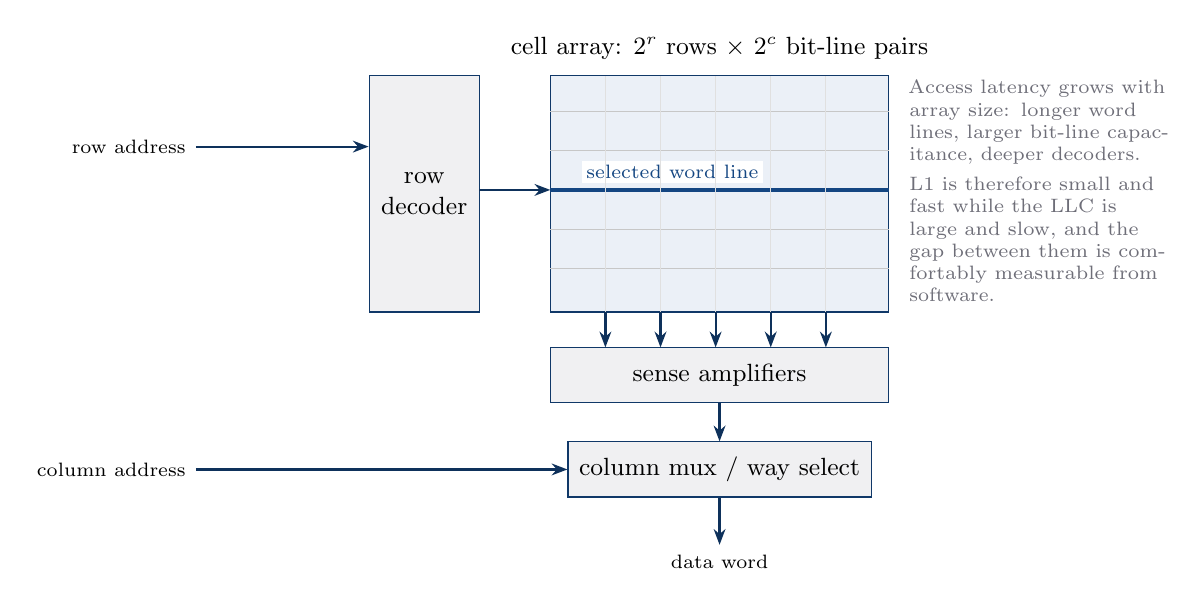
\begin{tikzpicture}[scale=1.0]
  % --- decoder -------------------------------------------------------
  \node[memblk, minimum width=1.4cm, minimum height=3.0cm, align=center] (dec) at (0,0)
        {row\\decoder};
  % --- array box -----------------------------------------------------
  \draw[draw=accent!80!black, fill=lightfill] (1.6,-1.5) rectangle (5.9,1.5);
  \node[font=\small] at (3.75,1.85) {cell array: $2^{r}$ rows $\times$ $2^{c}$ bit-line pairs};
  % rows inside the array
  \foreach \y in {1.05,0.55,-0.45,-0.95} {\draw[black!22] (1.6,\y) -- (5.9,\y);}
  \draw[accent, very thick] (1.6,0.05) -- (5.9,0.05);
  \node[note, anchor=west, text=accent] at (2.0,0.28) {selected word line};
  % columns inside the array
  \foreach \x in {2.3,3.0,3.7,4.4,5.1} {\draw[black!12] (\x,-1.5) -- (\x,1.5);}
  % decoder to array
  \draw[sig] (0.7,0.05) -- (1.6,0.05);
  % --- sense amps and mux ---------------------------------------------
  \node[memblk, minimum width=4.3cm, minimum height=0.7cm] (sa) at (3.75,-2.3) {sense amplifiers};
  \foreach \x in {2.3,3.0,3.7,4.4,5.1} {\draw[sig] (\x,-1.5) -- (\x,-1.95);}
  \node[memblk, minimum width=2.8cm, minimum height=0.7cm] (mux) at (3.75,-3.5) {column mux / way select};
  \draw[sig] (sa.south) -- (mux.north);
  \draw[sig] (mux.south) -- ++(0,-0.6) node[below, font=\scriptsize] {data word};
  % --- address inputs ---------------------------------------------------
  \draw[sig] (-2.9,0.6) node[left, font=\scriptsize] {row address} -- (dec.west|-,0.6);
  \draw[sig] (-2.9,-3.5) node[left, font=\scriptsize] {column address} -- (mux.west);
  % --- annotation --------------------------------------------------------
  \node[note, anchor=north west, text width=3.25cm] at (6.1,1.5)
        {Access latency grows with array size: longer word lines, larger
         bit-line capacitance, deeper decoders.\\[3pt]
         L1 is therefore small and fast while the LLC is large and slow, and the gap
         between them is comfortably measurable from software.};
\end{tikzpicture}%
}
\caption[Array organisation]{Organisation of an SRAM array (textbook
\SecRef{7.4.1}). Every cache, TLB, branch target buffer and predictor table in
\Cref{ch:memsys,ch:pipeline} is one or more instances of this structure, with
different tag and comparison logic wrapped around it.}
\label{fig:array}
\end{figure}

\Cref{fig:readtiming} shows the same access in time. The sequence (precharge,
assert the word line, wait for a differential to develop, fire the sense
amplifier, drive the output) is what a ``one cycle'' L1 access actually
contains.

\begin{figure}[t]
\centering
\small
\begin{tikztimingtable}[timing/slope=0.08, xscale=2.4, yscale=1.5,
                        timing/rowdist=3.2ex,
                        timing/name/.style={font=\scriptsize}]
  \texttt{CLK}                  & 8{C} \\
  Precharge                     & 3H 3L 2H \\
  Word line \texttt{WL}         & 3L 4H 1L \\
  BL, $\overline{\text{BL}}$    & 3D{precharged} 3X 2D{$\Delta V$ resolved} \\
  Sense enable                  & 5L 2H 1L \\
  Data out                      & 5Z 1X 2D{valid} \\
\end{tikztimingtable}
\par\vspace{2pt}
\caption[Read timing of an SRAM array]{Timing of a single array read (textbook
\SecRef{7.4.1}), drawn programmatically with \texttt{tikz-timing}. The
observable quantity in every attack in this paper is the horizontal distance
from the request to ``data valid'', and that distance is different for an L1
hit, an L2 hit, an LLC hit and a DRAM access by amounts that are large compared
with the resolution of \texttt{rdcycle}.}
\label{fig:readtiming}
\end{figure}

\begin{takeaway}[unbreakable]
The timing difference exploited by every cache attack is not a subtle artefact.
It is the direct, intended consequence of building small fast arrays close to
the pipeline and large slow arrays further away. Any implementation that removes
the difference gives up the reason for having a hierarchy at all.
\end{takeaway}

\section{The same array, wearing different hats}

The structures that leak in \Cref{ch:memsys,ch:pipeline,ch:multicore} are all
instances of \Cref{fig:array} with different wrappers.
\Cref{tab:arrayzoo} lists them with representative parameters for an
application-class RISC-V core in the style of CVA6~\citep{zaruba2019ariane} or
BOOM~\citep{zhao2020sonicboom}.

\begin{table}[t]
\centering
\caption[Array-based structures in a RISC-V core]{Array-based structures in a
representative application-class RISC-V core, the wrapper logic each one carries,
and the reason each is a candidate transmitter. Sizes are representative
configuration values, not measurements.}
\label{tab:arrayzoo}
\footnotesize
\begin{tabularx}{\linewidth}{@{}>{\raggedright\arraybackslash}p{2.9cm}>{\raggedright\arraybackslash}p{2.5cm}>{\raggedright\arraybackslash}p{1.9cm}X@{}}
\toprule
\textbf{Structure} & \textbf{Wrapper logic} & \textbf{Typical size} & \textbf{Why it transmits} \\
\midrule
L1 data cache      & tag compare, way mux, LRU update & 32\,KiB, 8-way &
Hit/miss latency gap of tens of cycles; index is a function of the address. \\
L1 instruction cache & tag compare, prefetch  & 32\,KiB, 8-way &
Reveals executed code path at line granularity. \\
L2 / LLC           & tags, coherence directory & 512\,KiB--8\,MiB &
Shared across cores; the basis of cross-core attacks (tier T3). \\
Data TLB           & fully-associative CAM, ASID compare & 32--64 entries &
Reveals accessed \emph{page}; survives context switch when ASID-tagged. \\
Page-walk cache    & tag compare on PTE address & 16--32 entries &
Leaks intermediate page-table levels, hence pointer values. \\
Branch direction predictor & indexed by PC $\oplus$ history & 4--16\,Kib &
One bit of outcome per branch; aliasing makes it cross-domain. \\
Branch target buffer & tag compare on PC & 512--4096 entries &
Leaks target addresses; enables branch-target injection. \\
Return address stack & shift-register array & 8--32 entries &
Leaks call depth; mistraining redirects speculative returns. \\
MSHRs / line-fill buffers & address CAM & 4--16 entries &
Contention reveals in-flight misses even without cache-state change. \\
Store buffer / LSQ & address CAM for forwarding & 16--64 entries &
Address-match forwarding creates a data-dependent timing path. \\
\bottomrule
\end{tabularx}
\end{table}

Note the recurrence of \emph{content-addressable} structures, the subject of
\SecRef{7.4.2}. A CAM compares a key against every stored entry in parallel\index{content-addressable memory (CAM)}; TLBs, MSHRs and store queues use
them because they need associative lookup. A CAM's timing depends on whether a
match occurred, and matching depends on addresses, which depend on data. Every
CAM in a processor is a candidate for an address-dependent timing path, which is
why store-to-load forwarding turned out to be exploitable (Spectre-v4) and why\index{store-to-load forwarding}
MSHR contention is a channel even when no cache line changes state.

\section{Why an array access is never constant-time in situ}

Even holding the array itself constant, several implementation techniques make
the observed latency of an access depend on state that an attacker can
influence:

\begin{itemize}
  \item \textbf{Banking and port conflicts.} Multi-banked L1s serve two accesses
        per cycle only if they fall in different banks. Bank conflicts are a
        function of address bits, hence of data.
  \item \textbf{Way prediction.} To save energy, some cores predict the way and
        read only one; a misprediction costs an extra cycle. The predictor is
        indexed by address, so the extra cycle is an address-dependent signal.
  \item \textbf{Error-correcting codes.} An ECC correction event costs extra
        cycles and depends on stored data.
  \item \textbf{Miss-status holding registers.} A miss to a line already being
        fetched merges into an existing MSHR (cheap) or allocates a new one\index{miss-status holding register (MSHR)}
        (possibly stalling if none are free). Occupancy is attacker-influenceable.
  \item \textbf{Replacement metadata.} An LRU update is a write to a small array;
        its state after a victim's access is what Prime+Probe reads
        (\Cref{ch:memsys}).
\end{itemize}

\begin{takeaway}
Constant-time \emph{code} is not the same thing as constant-time
\emph{execution}. A programmer can eliminate secret-dependent branches and
secret-dependent addresses, and the hardware can still produce\index{constant-time code!versus constant-time execution}
secret-\emph{correlated} timing through banking, way prediction, ECC, or MSHR
contention. It is the reason architectural promises such as \texttt{Zkt}~\citep{riscv-crypto} are scoped narrowly to data-operand
independence: broader promises would be very hard for an implementation to keep.
\end{takeaway}

\begin{draftnote}
For v0.2 this chapter gains: (a) a short quantitative model relating array size
to access latency, in the style of CACTI, so that \Cref{ch:tradeoffs} can price
the extra tag bits required by partitioned and randomised caches;
(b) a figure showing a set-associative tag/data array pair with the way-mux
critical path highlighted; and (c) a paragraph on the DRAM organisation of \SecRef{7.4.3} and its row buffers,
for completeness of the ``arrays that remember'' theme. Target: +2 pages.
\end{draftnote}

\chapter{The Reference Machine: Datapath and Control}
\label{ch:proc}

\begin{tocmapbox}
Background: textbook \SecRef{9.1} (design of a basic processor), \SecRef{9.2}
(units in a processor) with \SecRef{9.2.1}--\SecRef{9.2.7} (fetch unit; data path
and control path; operand fetch unit; execute unit; memory access unit; register
writeback unit; the data path) and \SecRef{9.3} (the control
unit)~\citep{sarangi2025basic}.
\end{tocmapbox}

\section{Purpose of this chapter}

Everything that follows (pipelining, speculation, caches, coherence) is an
optimisation applied to one simple machine. This chapter fixes that machine so
that later chapters can say precisely \emph{what was added} and \emph{what the
addition leaked}. The reference is a single-cycle RV64I datapath, in the style
of textbook \SecRef{9.2}, mapped onto the RISC-V instruction formats of
\Cref{fig:encoding}.

The security claim of this chapter is deliberately modest, and it is a negative
one: \textbf{the machine of \Cref{fig:datapath}, taken literally, has almost no
\uarchadj{} channels.} It has no cache, no predictor, no speculation and no
sharing. Its timing is a function of the instruction opcode alone. Establishing
that baseline is what makes it possible to attribute each later channel to a
specific optimisation, rather than to ``hardware'' in general.

\section{The single-cycle datapath}

\begin{figure}[t]
\centering
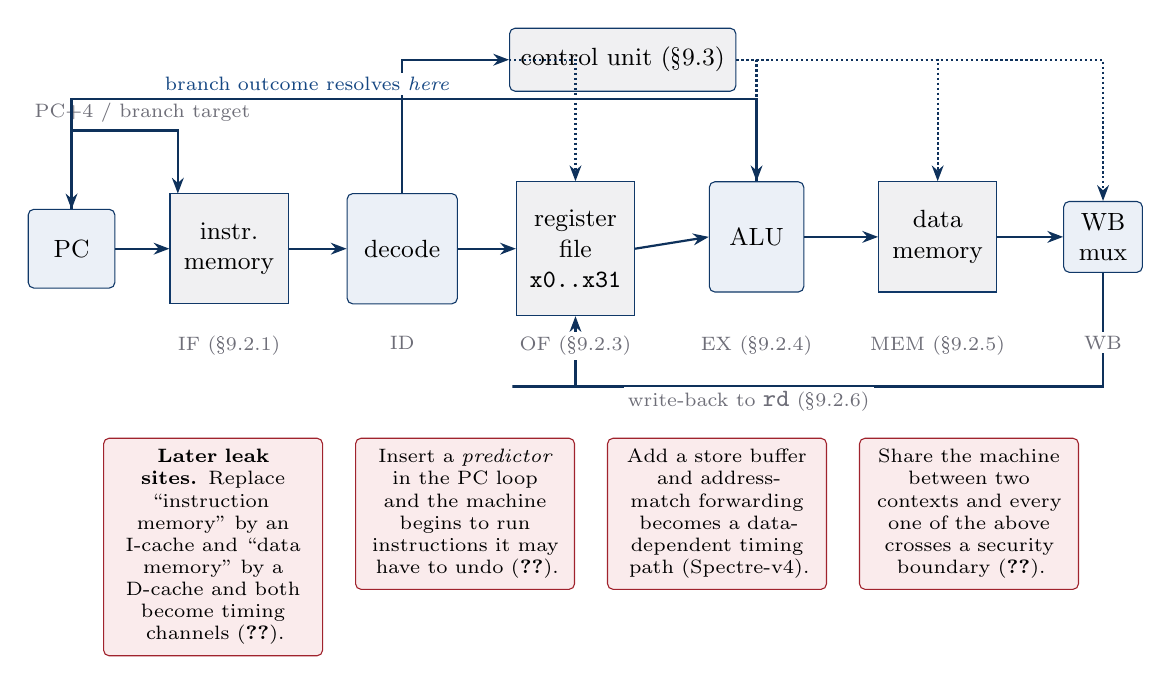
\begin{tikzpicture}[scale=1.0, every node/.style={font=\scriptsize}]
  % ---- stage blocks ------------------------------------------------
  \node[blk, minimum width=1.1cm, minimum height=1.0cm] (pc)  at (0,0)     {PC};
  \node[memblk, minimum width=1.5cm, minimum height=1.4cm] (imem) at (2.0,0) {instr.\\memory};
  \node[blk, minimum width=1.4cm, minimum height=1.4cm] (dec) at (4.2,0)   {decode};
  \node[memblk, minimum width=1.5cm, minimum height=1.7cm] (rf) at (6.4,0)  {register\\file\\\code{x0..x31}};
  \node[blk, minimum width=1.2cm, minimum height=1.4cm] (alu) at (8.7,0.15) {ALU};
  \node[memblk, minimum width=1.5cm, minimum height=1.4cm] (dmem) at (11.0,0.15){data\\memory};
  \node[blk, minimum width=1.0cm, minimum height=0.9cm] (wb)  at (13.1,0.15) {WB\\mux};

  % ---- control unit -------------------------------------------------
  \node[blk, minimum width=2.4cm, minimum height=0.8cm, fill=greyfill] (ctrl) at (7.0,2.4)
       {control unit (\SecRef{9.3})};
  \draw[sig] (dec.north) |- (ctrl.west);
  \foreach \t in {alu, dmem, wb} {\draw[sig, densely dotted] (ctrl.east) -| (\t.north);}
  \draw[sig, densely dotted] (ctrl.west) -| (rf.north);

  % ---- datapath wires ------------------------------------------------
  \draw[sig] (pc)   -- (imem);
  \draw[sig] (imem) -- (dec);
  \draw[sig] (dec)  -- (rf);
  \draw[sig] (rf.east)  -- (alu.west);
  \draw[sig] (alu.east) -- (dmem.west);
  \draw[sig] (dmem.east) -- (wb.west);
  % write-back path
  \draw[sig] (wb.south) |- (5.6,-1.75) -| (rf.south);
  \node[note, anchor=north] at (8.6,-1.75) {write-back to \code{rd} (\SecRef{9.2.6})};
  % PC + 4 loop
  \draw[sig] (pc.north) |- (0.9,1.5) -| (1.35,0.7);
  \node[note, anchor=south] at (0.9,1.55) {PC$+4$ / branch target};
  % branch resolution feedback
  \draw[sig] (alu.north) |- (5.0,1.9) -| (0,0.5);
  \node[note, anchor=south, text=accent] at (3.0,1.95) {branch outcome resolves \emph{here}};

  % ---- stage labels --------------------------------------------------
  \foreach \x/\l in {2.0/{IF (\SecRef{9.2.1})}, 4.2/{ID}, 6.4/{OF (\SecRef{9.2.3})},
                     8.7/{EX (\SecRef{9.2.4})}, 11.0/{MEM (\SecRef{9.2.5})}, 13.1/{WB}}
     {\node[note, anchor=north] at (\x,-1.05) {\l};}

  % ---- security annotations -------------------------------------------
  \node[atk, font=\scriptsize, text width=2.5cm, anchor=north west] at (0.4,-2.4)
       {\textbf{Later leak sites.} Replace ``instruction memory'' by an I-cache and
        ``data memory'' by a D-cache and both become timing channels
        (\Cref{ch:memsys}).};
  \node[atk, font=\scriptsize, text width=2.5cm, anchor=north west] at (3.6,-2.4)
       {Insert a \emph{predictor} in the PC loop and the machine begins to run
        instructions it may have to undo (\Cref{ch:pipeline}).};
  \node[atk, font=\scriptsize, text width=2.5cm, anchor=north west] at (6.8,-2.4)
       {Add a store buffer and address-match forwarding becomes a data-dependent
        timing path (Spectre-v4).};
  \node[atk, font=\scriptsize, text width=2.5cm, anchor=north west] at (10.0,-2.4)
       {Share the machine between two contexts and every one of the above
        crosses a security boundary (\Cref{ch:multicore}).};
\end{tikzpicture}
\caption[Single-cycle RISC-V datapath]{The reference single-cycle RV64I datapath
(textbook \SecRef{9.2}), with the control path of \SecRef{9.3} shown dotted. As
drawn, this machine has essentially no \uarchadj{} side channels: memory is a flat
array with fixed latency, the branch outcome is known before the next fetch, and
nothing is shared. The four red boxes name the optimisations that later chapters
add, and the channel each one opens.}
\label{fig:datapath}
\end{figure}

\subsection{Stage by stage}

\paragraph{Instruction fetch (\SecRef{9.2.1}).} The PC addresses instruction
memory; the fetched word is the instruction. In the reference machine the PC
update is $\text{PC} \leftarrow \text{PC}+4$ or a computed target, and the choice
is made \emph{after} the branch condition is known. This is the property that
pipelining destroys.

\paragraph{Decode and operand fetch (\SecRef{9.2.2}, \SecRef{9.2.3}).} Because
the register specifiers occupy fixed positions in every format
(\Cref{fig:encoding}), the register file can be read in parallel with decoding.
The immediate is extracted and sign-extended according to format.

\paragraph{Execute (\SecRef{9.2.4}).} The ALU computes an
arithmetic result, an effective address, or a branch condition. One functional
unit, one result per cycle, no reordering.

\paragraph{Memory access (\SecRef{9.2.5}).} Loads read and stores write the data
memory. In the reference machine this takes a fixed time. \emph{The entire
subject of \Cref{ch:memsys} is what happens when it does not.}

\paragraph{Register write-back (\SecRef{9.2.6}).} The result is written to
\code{rd}, or discarded if the instruction has no destination. After write-back
the architectural state is exactly what \Cref{eq:contract} requires.

\subsection{The control path}

The control unit of \SecRef{9.3} (``The Control Unit'') decodes the opcode and the \code{funct} fields
into the mux selects and enables that steer the datapath. In a single-cycle
machine, control is a pure combinational function of the current instruction. It
has no memory, and therefore no history, which is again what later optimisations
change. A branch predictor is nothing other than a control unit
with memory, and memory is what leaks.

\section{Where security-relevant state will appear}

\Cref{tab:stagestate} walks the same six stages and, for each, names the
structure that a high-performance implementation adds, the information it
retains, and the chapter in which the resulting channel is analysed. It is the
roadmap of the technical half of this paper.

\begin{table}[t]
\centering
\caption[Pipeline stages and the state added by optimisation]{The six stages of
the reference machine, the \uarchadj{} structures a high-performance
implementation adds to each, and where in this paper the resulting channel is
analysed.}
\label{tab:stagestate}
\footnotesize
\begin{tabularx}{\linewidth}{@{}p{2.1cm}p{4.0cm}Xp{1.6cm}@{}}
\toprule
\textbf{Stage} & \textbf{Structure added} & \textbf{Information retained} & \textbf{Analysed in} \\
\midrule
Fetch    & I-cache, BTB, RAS, direction predictor &
Which lines were fetched; which branches were taken; call/return targets &
\Cref{ch:pipeline,ch:memsys} \\
Decode   & Micro-op cache, decoded-instruction buffers &
Which instructions were decoded recently & \Cref{ch:pipeline} \\
Operand fetch & Physical register file, rename map, issue queue &
Occupancy and readiness, hence dependence structure & \Cref{ch:pipeline} \\
Execute  & Multiple functional units, bypass network, execution window &
Port contention; which units were busy & \Cref{ch:pipeline,ch:transient} \\
Memory   & D-cache, TLB, page-walk cache, store buffer, LSQ, MSHRs &
Which lines and pages were touched; address matches for forwarding &
\Cref{ch:memsys} \\
Write-back & Reorder buffer, commit logic &
Retirement order and squash events (timing only) & \Cref{ch:pipeline,ch:transient} \\
\bottomrule
\end{tabularx}
\end{table}

\begin{takeaway}
The reference machine is secure against \uarchadj{} attacks and unusably slow. Every
structure that makes it fast is a structure that remembers something about what
ran before. The design question this paper ends on (\Cref{ch:tradeoffs}) is not
``can we remove the channels'' (we can, by returning to \Cref{fig:datapath}) but ``how much performance must we return to close a given
channel''.
\end{takeaway}

\begin{draftnote}
For v0.2: add a second figure showing the same datapath annotated with the actual
module boundaries of an open RISC-V implementation (Rocket's
\texttt{RocketCore} stages, or CVA6's six stages), so that the abstract textbook
datapath is tied to code the reader can inspect. Also add a short subsection on
the RISC-V privilege model in the datapath (\code{mstatus}, trap vectors), which
\Cref{ch:transient} needs when discussing Meltdown-type faults. Target: +2.5 pages.
\end{draftnote}

\chapter{Pipelining, Speculation and the Birth of Transient State}
\label{ch:pipeline}

\begin{tocmapbox}
Background: textbook \SecRef{10.1}--\SecRef{10.3} (the pipelined processor and
its stages), \SecRef{10.4} (pipeline hazards), \SecRef{10.8} (support for
interrupts and exceptions) with \SecRef{10.8.2} (exceptions) and \SecRef{10.8.3}
(precise exceptions), \SecRef{10.9.3} (performance of a non-ideal pipeline),
\SecRef{10.10} (power and temperature issues), and \SecRef{10.11} (advanced
techniques) with \SecRef{10.11.1} (branch prediction) and \SecRef{10.11.4}
(out-of-order pipelines)~\citep{sarangi2025basic}.
\end{tocmapbox}

This is the first of the two chapters that carry the weight of the paper. It
introduces the two properties that turn passive timing differences into an
active, steerable read primitive: \emph{speculation} (the machine executes
instructions before it knows they are needed) and \emph{squashing} (the machine
can erase their architectural effects but not their \uarchadj{} ones).

\section{The pipeline}

\Cref{fig:pipeline} shows the classic five-stage pipeline of \SecRef{10.2},
which is essentially the organisation of the Rocket\index{Rocket core}
core~\citep{asanovic2016rocket}. Pipeline registers between stages hold the
in-flight instruction's state; up to five instructions are in flight at once.\index{pipeline!five-stage}

\begin{figure}[t]
\centering
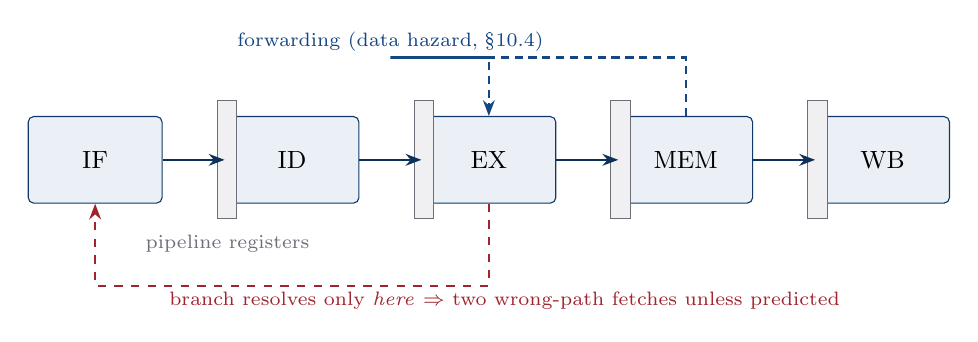
\begin{tikzpicture}[scale=1.0, every node/.style={font=\scriptsize}]
  \foreach \i/\x/\n in {0/0/IF, 1/2.5/ID, 2/5.0/EX, 3/7.5/MEM, 4/10.0/WB}
    {\node[blk, minimum width=1.7cm, minimum height=1.1cm] (s\i) at (\x,0) {\n};}
  \foreach \i/\x in {0/1.55, 1/4.05, 2/6.55, 3/9.05}
    {\draw[fill=greyfill, draw=muted] (\x,-0.75) rectangle ++(0.25,1.5);}
  \foreach \i [evaluate=\i as \j using int(\i+1)] in {0,1,2,3}
    {\draw[sig] (s\i.east) -- (s\j.west);}
  \node[note, anchor=north] at (1.68,-0.9) {pipeline registers};

  % hazards
  \draw[sig, densely dashed, draw=accent] (s3.north) |- (3.75,1.3) -| (s2.north);
  \node[note, anchor=south, text=accent] at (3.75,1.32) {forwarding (data hazard, \SecRef{10.4})};
  \draw[atksig] (s2.south) |- (2.5,-1.6) -| (s0.south);
  \node[note, anchor=north, text=attack] at (5.2,-1.62)
       {branch resolves only \emph{here} $\Rightarrow$ two wrong-path fetches unless predicted};
\end{tikzpicture}
\caption[Five-stage pipeline]{The five-stage pipeline of textbook
\SecRef{10.2}--\SecRef{10.3}. Forwarding paths resolve data hazards; the branch
outcome, however, is not known until EX, so the fetch stage must either stall or
\emph{guess}. Guessing is the origin of everything in \Cref{ch:transient}.}
\label{fig:pipeline}
\end{figure}

\subsection{Hazards and the pressure to speculate}

Textbook \SecRef{10.4} classifies the three hazards; \Cref{tab:hazards}
summarises them together with the \uarchadj{} consequence that matters here.

\begin{table}[b]
\centering
\caption[Hazards and their security consequence]{The three hazard classes
(\SecRef{10.4}), their standard resolution, and the security-relevant residue
each resolution leaves behind.}
\label{tab:hazards}
\footnotesize
\begin{tabularx}{\linewidth}{@{}p{2.2cm}p{4.2cm}X@{}}
\toprule
\textbf{Hazard} & \textbf{Standard resolution} & \textbf{Security-relevant residue} \\
\midrule
Data (RAW) & Forwarding; interlock and stall when a load feeds the next instruction &
Stall cycles are visible in timing; store-to-load forwarding is an
address-comparison whose outcome is data-dependent (Spectre-v4). \\
Control & Predict the branch; squash wrong-path instructions when the prediction
is resolved &
Wrong-path instructions \emph{execute} before being squashed. Their \uarchadj{}
effects are not undone. Spectre is built on that. \\
Structural & Duplicate the resource, or arbitrate &
Arbitration makes one context's timing depend on another's resource use, the mechanism of SMT and port-contention channels. \\
\bottomrule
\end{tabularx}
\end{table}

\subsection{Branch prediction}

To avoid stalling on every control hazard, the fetch stage predicts. A modern\index{branch prediction}
RISC-V core such as SonicBOOM~\citep{zhao2020sonicboom} carries a hierarchy of
predictors, sketched in \Cref{fig:predictors}: a direction predictor indexed by a
hash of PC and global history, a branch target buffer, and a return address
stack.

\begin{figure}[t]
\centering
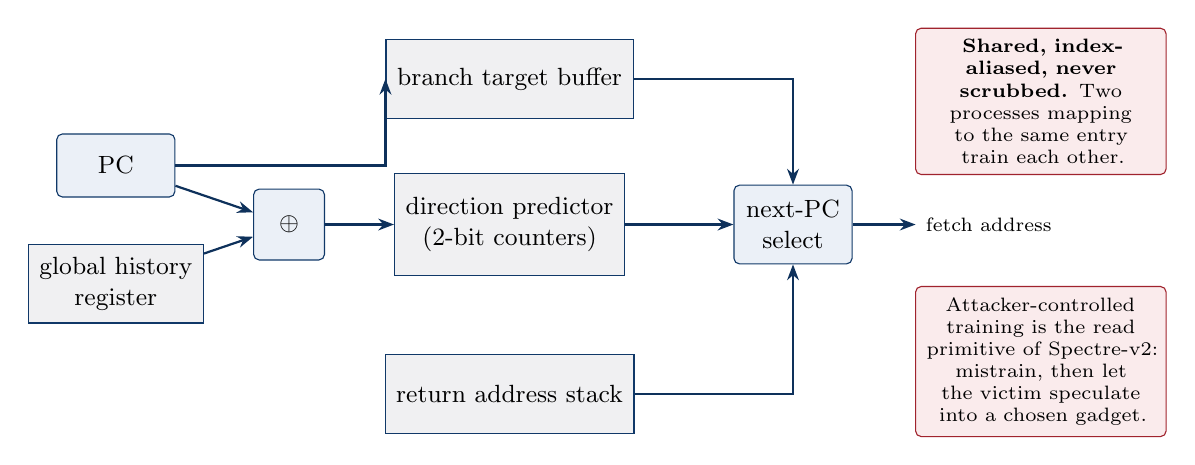
\begin{tikzpicture}[scale=1.0, every node/.style={font=\scriptsize}]
  \node[blk, minimum width=1.5cm] (pc) at (0,0) {PC};
  \node[memblk, minimum width=1.9cm, minimum height=1.0cm] (ghr) at (0,-1.5) {global history\\register};
  \node[blk, minimum width=0.9cm, minimum height=0.9cm] (xor) at (2.2,-0.75) {$\oplus$};
  \node[memblk, minimum width=2.3cm, minimum height=1.3cm] (bht) at (5.0,-0.75)
       {direction predictor\\(2-bit counters)};
  \node[memblk, minimum width=2.3cm, minimum height=1.0cm] (btb) at (5.0,1.1) {branch target buffer};
  \node[memblk, minimum width=2.3cm, minimum height=1.0cm] (ras) at (5.0,-2.9) {return address stack};
  \node[blk, minimum width=1.5cm, minimum height=1.0cm] (nxt) at (8.6,-0.75) {next-PC\\select};

  \draw[sig] (pc) -- (xor); \draw[sig] (ghr) -- (xor);
  \draw[sig] (xor) -- (bht);
  \draw[sig] (pc.east) -| (btb.west);
  \draw[sig] (bht) -- (nxt); \draw[sig] (btb.east) -| (nxt.north);
  \draw[sig] (ras.east) -| (nxt.south);
  \draw[sig] (nxt.east) -- ++(0.8,0) node[right] {fetch address};

  %% Anchored north/south so the two callouts grow away from each other; the
  %% atk style would otherwise override the picture-wide \scriptsize and collide.
  \node[atk, text width=2.9cm, font=\scriptsize, anchor=north west] at (10.15,1.75)
       {\textbf{Shared, index-aliased, never scrubbed.} Two processes mapping to
        the same entry train each other.};
  \node[atk, text width=2.9cm, font=\scriptsize, anchor=south west] at (10.15,-3.45)
       {Attacker-controlled training is the read primitive of Spectre-v2:
        mistrain, then let the victim speculate into a chosen gadget.};
\end{tikzpicture}
\caption[Branch prediction structures]{Branch prediction structures
(\SecRef{10.11.1}). The direction predictor is indexed by a hash of the PC and
global history, so entries alias between unrelated branches, including
branches in different processes or privilege levels. The BTB and RAS supply
targets. All three are \uarchadj{} state by the definition of
\Cref{sec:archvsuarch}: nothing restores them on a context switch.}
\label{fig:predictors}
\end{figure}

Prediction accuracy above 95\,\% is routine, and that accuracy is what makes deep
pipelines and wide issue worthwhile. The security cost is
structural: a predictor is a shared, index-aliased, persistent memory that any\index{predictor!aliasing between domains}
context can write and whose effects any context can observe through timing.
Evtyushkin \etal{} showed that the directional predictor alone is a usable
channel~\citep{evtyushkin2018branchscope}, and branch-history injection
demonstrated that partial isolation of these structures is not enough when the\index{Spectre!v2, branch target injection}
history register itself is shared~\citep{barberis2022bhi}.

\section{Precise exceptions do not undo microarchitectural effects}
\label{sec:precise}

Textbook \SecRef{10.8.3} defines a \emph{precise} exception: when an exception
is taken, all instructions before the faulting one have completed, none after it\index{precise exceptions}
has had any effect, and the architectural state is exactly as if the program had
stopped at that instruction. Precise exceptions are what make debugging,
virtual memory and context switching tractable, and RISC-V requires
them~\citep{riscv-priv}.

The definition quantifies over \emph{architectural} state only, because when
the mechanism was standardised in the form we still use~\citep{smith1988precise},
that was the only state anyone had reason to care about. \Cref{fig:squash} makes
the consequence concrete, and it also shows why the five-stage machine is not yet
enough for an attack: the asymmetry is real at every pipeline depth, but the size
of the window it opens is not.

\begin{figure}[t]
\centering
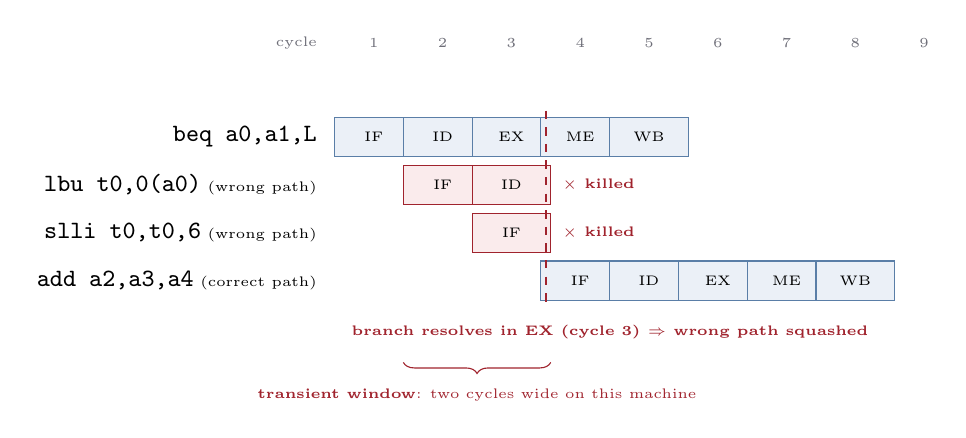
\begin{tikzpicture}[scale=0.78, every node/.style={font=\scriptsize}]
  % column headers
  \foreach \c in {1,...,9} {\node[text=muted, font=\tiny] at (\c*1.12, 0.75) {\c};}
  \node[anchor=east, text=muted, font=\tiny] at (0.35,0.75) {cycle};
  % rows: row / label / first cycle / stages actually completed / 1 = wrong path
  \foreach \r/\name/\start/\nst/\bad in {%
      1/{\code{beq a0,a1,L}}/1/5/0,
      2/{\code{lbu t0,0(a0)} (wrong path)}/2/2/1,
      3/{\code{slli t0,t0,6} (wrong path)}/3/1/1,
      4/{\code{add a2,a3,a4} (correct path)}/4/5/0}
  {
    \node[anchor=east, font=\tiny] at (0.35,-\r*0.78) {\name};
    \foreach \s [count=\i from 0] in {IF,ID,EX,ME,WB}
    {
      \ifnum\i<\nst\relax
        \pgfmathsetmacro{\cx}{(\start+\i)*1.12}
        \ifnum\bad=1\relax
          \node[draw=attack, fill=attackfill, minimum width=1.0cm, minimum height=0.5cm,
                inner sep=0pt, font=\tiny] at (\cx,-\r*0.78) {\s};
        \else
          \node[draw=accent!70, fill=lightfill, minimum width=1.0cm, minimum height=0.5cm,
                inner sep=0pt, font=\tiny] at (\cx,-\r*0.78) {\s};
        \fi
      \fi
    }
    % "killed here" marker for the wrong-path rows
    \ifnum\bad=1\relax
      \pgfmathsetmacro{\kx}{(\start+\nst)*1.12}
      \node[text=attack, font=\tiny\bfseries, anchor=west] at (\kx-0.45,-\r*0.78)
            {$\times$ killed};
    \fi
  }
  % squash marker: end of cycle 3
  \draw[attack, thick, dashed] (3.92,-0.35) -- (3.92,-3.55);
  \node[anchor=west, text=attack, font=\tiny\bfseries] at (0.6,-3.95)
       {branch resolves in EX (cycle~3) $\Rightarrow$ wrong path squashed};
  % transient window brace: the two wrong-path fetches, cycles 2--3
  \draw[decorate, decoration={brace, amplitude=4pt, mirror}, attack]
       (1.6,-4.45) -- (4.0,-4.45)
       node[midway, below=6pt, text=attack, align=center, font=\tiny]
       {\textbf{transient window}: two cycles wide on this machine};
\end{tikzpicture}
\caption[Squashed instructions leave state behind]{Pipeline diagram of a
mispredicted branch on the five-stage machine of \Cref{fig:pipeline}. The branch
resolves in EX at the end of cycle~3, so the two wrong-path instructions (red)
are killed in ID and in IF and never reach the memory stage. Precise exception
semantics (\SecRef{10.8.3}) guarantee that their \emph{architectural} effects
vanish; what does \emph{not} vanish is the instruction-cache line fetched for the
wrong path and the predictor entry that sent the machine there. Driving the
\emph{data} cache transiently, which is the transmitter of \Cref{ch:transient},
needs a window far wider than two cycles, and \Cref{sec:ooo} shows where that
window comes from.}
\label{fig:squash}
\end{figure}

\begin{takeaway}
Squashing is architecturally complete and \uarchadv{} partial. A processor that
made squashing complete in both senses (restoring cache, TLB, predictor and
buffer state on every misprediction) would be secure against Spectre and would
also be slow, because the recovery cost would apply to the 5\,\% of branches that
mispredict. \Cref{ch:defenses} shows that most real defences are attempts to make
the undo cheap (CleanupSpec~\citep{saileshwar2019cleanupspec}) or to make the
effect invisible in the first place (InvisiSpec~\citep{yan2018invisispec}).
\end{takeaway}

\section{Out-of-order execution and the size of the window}
\label{sec:ooo}

Textbook \SecRef{10.11.4} introduces out-of-order execution: instructions are
renamed, dispatched into issue queues, executed as soon as their operands are\index{out-of-order execution}
ready, and retired in program order from a reorder buffer.\index{reorder buffer (ROB)}
\Cref{fig:ooo} sketches the organisation and marks the structures relevant to
this paper.

\begin{figure}[t]
\centering
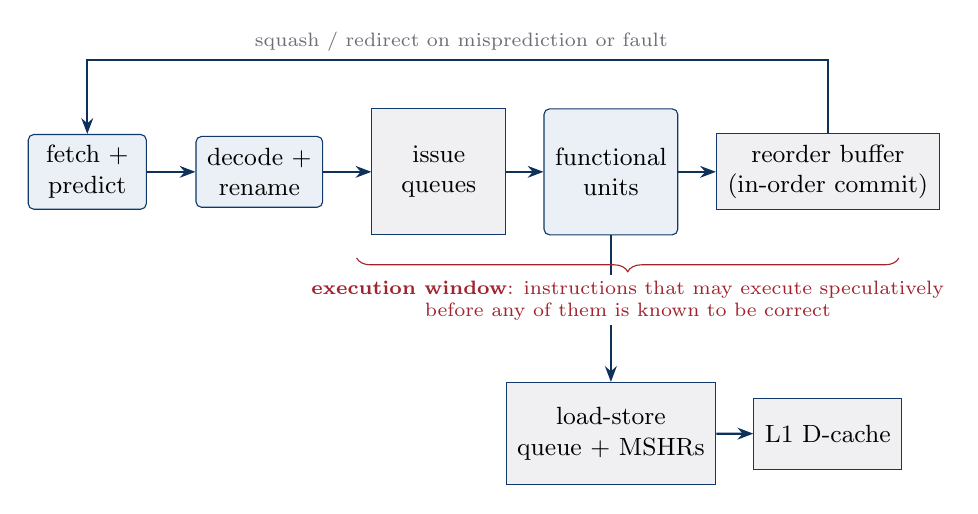
\begin{tikzpicture}[scale=0.95, every node/.style={font=\scriptsize}]
  \node[blk, minimum width=1.5cm, minimum height=0.9cm] (fe) at (0,0) {fetch +\\predict};
  \node[blk, minimum width=1.5cm, minimum height=0.9cm] (rn) at (2.3,0) {decode +\\rename};
  \node[memblk, minimum width=1.7cm, minimum height=1.6cm] (iq) at (4.7,0) {issue\\queues};
  \node[blk, minimum width=1.5cm, minimum height=1.6cm] (fu) at (7.0,0) {functional\\units};
  \node[memblk, minimum width=1.7cm, minimum height=1.3cm] (lsq) at (7.0,-3.5) {load-store\\queue + MSHRs};
  \node[memblk, minimum width=1.9cm, minimum height=0.9cm] (rob) at (9.9,0) {reorder buffer\\(in-order commit)};
  \node[memblk, minimum width=1.7cm, minimum height=0.9cm] (dc) at (9.9,-3.5) {L1 D-cache};

  \draw[sig] (fe)--(rn); \draw[sig] (rn)--(iq); \draw[sig] (iq)--(fu);
  \draw[sig] (fu)--(rob);
  \draw[sig] (fu.south)--(lsq.north);
  \draw[sig] (lsq)--(dc);
  \draw[sig] (rob.north) |- (5.0,1.5) -| (fe.north);
  \node[note, anchor=south] at (5.0,1.55) {squash / redirect on misprediction or fault};

  \draw[decorate, decoration={brace, amplitude=5pt, mirror}, attack]
       (3.6,-1.15) -- (10.85,-1.15)
       node[midway, below=6pt, text=attack, align=center, font=\scriptsize,
            fill=white, inner sep=2pt]
       {\textbf{execution window}: instructions that may execute speculatively\\
        before any of them is known to be correct};
\end{tikzpicture}
\caption[Out-of-order organisation]{Out-of-order organisation
(\SecRef{10.11.4}). The reorder buffer restores in-order, precise architectural
semantics on top of out-of-order execution. The width of the execution window (ROB entries, issue-queue entries, load-queue entries) determines how many
instructions can run transiently, and therefore how much work an attacker can
get done inside a single mis-speculation.}
\label{fig:ooo}
\end{figure}

The window size is the resource that matters for attack capability.\index{speculation window} An in-order
core such as Rocket squashes within a couple of cycles and can execute perhaps\index{in-order versus out-of-order cores}
one or two wrong-path instructions; an out-of-order core with a
100+\nobreakdash-entry ROB can execute a long dependent chain, which is why the
demonstrations on RISC-V hardware used BOOM rather than\index{BOOM (SonicBOOM) core}
Rocket~\citep{gonzalez2019replicating}. The same parameter that buys
instruction-level parallelism buys transient-attack bandwidth.

\begin{takeaway}
Attack capability scales with the \emph{same} \uarchadj{} parameters as performance:
window size, issue width, predictor accuracy, cache size, and sharing. This is
why there is no free defence, and why \Cref{ch:tradeoffs} is a required chapter
rather than an appendix.
\end{takeaway}

\section{Metrics: what a defence costs}
\label{sec:metrics}

Pricing a defence needs four quantities: execution time through the iron law,
relative slowdown against an insecure baseline, dynamic power, and the
energy-delay product that trades the first against the third. Their definitions,
and the conditions under which each is a valid comparison, run to more than half
a page and are therefore set out separately in \Cref{app:metrics}, which
\Cref{ch:tradeoffs} uses throughout. The one point that belongs here, next to the
speculation machinery that creates the cost, is negative: a slowdown quoted as a
ratio of IPCs is \emph{not} the same quantity as one quoted as a ratio of
execution times unless the defence leaves both the dynamic instruction count and
the clock frequency untouched, and several deployed defences leave neither.

\chapter{The Memory System as an Attack Surface}
\label{ch:memsys}

\begin{tocmapbox}
Background: textbook \SecRef{11.1.2}--\SecRef{11.1.8} (memory access patterns,
temporal and spatial locality, hierarchical memory, cache blocks), \SecRef{11.2}
(caches: lookup and design, read/write, insert, replace, evict), \SecRef{11.3}
(the memory system) with \SecRef{11.3.1} (its mathematical model), and
\SecRef{11.4} (virtual memory) with \SecRef{11.4.2} (the overlap and size
problems), \SecRef{11.4.3} (implementation of virtual memory with paging),
\SecRef{11.4.5} (the memory management unit) and \SecRef{11.4.6} (advanced
features of the paging system)~\citep{sarangi2025basic}.
\end{tocmapbox}

This is the second load-bearing chapter. Everything in \Cref{ch:memories}
explained why an array access takes time; everything in \Cref{ch:pipeline}
explained why a processor runs instructions it may have to undo. This chapter
combines the two into the measurement primitives that all real attacks use.

\section{Locality, hierarchy, and the size of the signal}

Caches exist because programs exhibit temporal locality (a recently used address\index{locality!temporal and spatial}
is likely to be used again) and spatial locality (an address near a recently used
one is likely to be used soon), as set out in
\SecRef{11.1.2}--\SecRef{11.1.5}. The hierarchy exploits this by placing a small
fast array close to the pipeline and progressively larger, slower arrays behind
it. \Cref{fig:hierarchy} plots representative access latencies for an
application-class RISC-V system.

\begin{figure}[t]
\centering
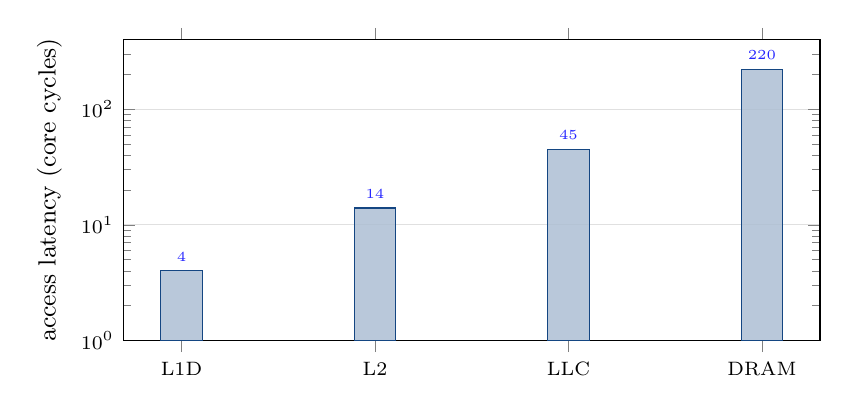
\begin{tikzpicture}
\begin{axis}[
  barstyle, height=5.4cm, width=0.86\linewidth,
  ybar, bar width=15pt,
  symbolic x coords={L1D,L2,LLC,DRAM},
  xtick=data, ymode=log, log basis y=10,
  ymin=1, ymax=400,
  ylabel={access latency (core cycles)},
  %% On a log axis pgfplots' default point meta is log10(y), so the bar labels
  %% must be given explicitly, otherwise they print 0.6, 1.15, ... not 4, 14, ...
  point meta=explicit symbolic,
  nodes near coords, nodes near coords style={font=\tiny},
  ]
  \addplot+[fill=accent!35, draw=accent] coordinates {
      (L1D,4) [4] (L2,14) [14] (LLC,45) [45] (DRAM,220) [220]};
\end{axis}
\end{tikzpicture}
\caption[Representative memory hierarchy latencies]{Representative access
latencies for the levels of the memory hierarchy in an application-class core,
on a logarithmic scale. \textbf{These are configuration-typical values used to
fix intuition, not measurements}; the author's own measured values for a
specific RISC-V configuration will replace them in v0.2
(\Cref{ch:evalplan}). The security-relevant point is the \emph{ratio}: an L1 hit
and a DRAM access differ by roughly a factor of 50, which is enormous compared
with the noise floor of a cycle counter.}
\label{fig:hierarchy}
\end{figure}

The attacker's signal is the difference between two of these bars.
\Cref{fig:hitmiss} draws that difference as a waveform on the core's load
interface, which is the form in which it is actually observed: the same
instruction, issued at the same cycle, returns its data at two very different
times.

\begin{figure}[t]
\centering
\small
\begin{tikztimingtable}[timing/slope=0.08, xscale=1.9, yscale=1.5,
                        timing/rowdist=3.2ex,
                        timing/name/.style={font=\scriptsize}]
  \texttt{clk}                          & 14{C} \\
  load issued (\code{lbu t2,0(t1)})     & L H 12L \\
  data returned, L1 \emph{hit}       & 4L H 9L \\
  data returned, L1 \emph{miss}      & 11L H 2L \\
  attacker's timer                      & 2D{\texttt{rdcycle}} 9D{measured interval} 3D{\texttt{rdcycle}} \\
\end{tikztimingtable}
\par\vspace{2pt}
\caption[Hit versus miss on the load interface]{The measurement, drawn on the
core's load interface. One load instruction, one issue cycle, two return times.
The attacker brackets the load with two reads of the cycle counter and
classifies the interval against a threshold; the horizontal gap between rows
three and four is the entire channel. The miss latency is drawn compressed; the true gap is far wider, as \Cref{fig:hierarchy} shows.}
\label{fig:hitmiss}
\end{figure}

No delicate measurement is required: distinguishing 4 cycles from 220 cycles is
trivial even with a coarse timer, and distinguishing an L2 hit from an LLC hit is
comfortable. Reducing timer resolution (a mitigation deployed in browsers) raises the number of repetitions needed but does not remove the difference, and
a counting thread reconstructs a fine-grained clock anyway.

\section{Cache organisation and the address split}

\SecRef{11.2} (``Caches'') develops the set-associative cache. A physical or virtual address
is split into three fields, as shown in \Cref{fig:addrsplit}: the block offset
selects a byte within a line, the index selects a set, and the tag is compared\index{cache!address split}
against the tags of all ways in that set.

\begin{figure}[t]
\centering
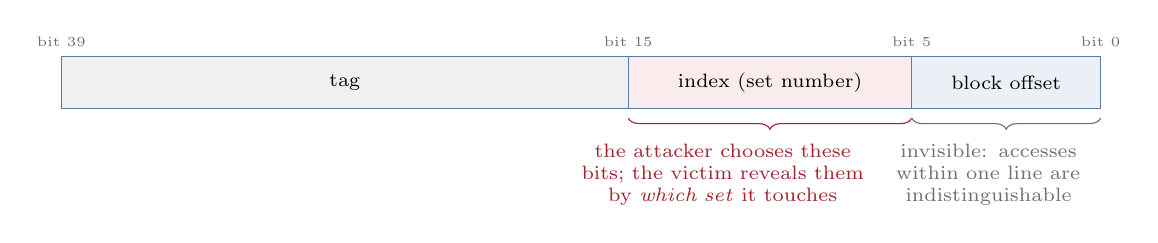
\begin{tikzpicture}[x=4.0mm, y=1cm]
  \newcommand{\afld}[5]{%
    \draw[fill=#5, draw=accent!70, line width=0.3pt] (#1,#2) rectangle ++(#3,0.66);
    \node[font=\scriptsize] at ({#1+#3/2}, {#2+0.33}) {#4};}
  \afld{0}{0}{18}{tag}{greyfill}
  \afld{18}{0}{9}{index (set number)}{attackfill}
  \afld{27}{0}{6}{block offset}{lightfill}
  \node[font=\tiny, text=muted] at (0,0.85) {bit 39};
  \node[font=\tiny, text=muted] at (18,0.85) {bit 15};
  \node[font=\tiny, text=muted] at (27,0.85) {bit 5};
  \node[font=\tiny, text=muted] at (33,0.85) {bit 0};
  % braces
  \draw[decorate, decoration={brace, amplitude=4pt, mirror}, attack] (18,-0.12) -- (27,-0.12);
  \draw[decorate, decoration={brace, amplitude=4pt, mirror}, muted]  (27,-0.12) -- (33,-0.12);
  % annotations, each kept inside its own horizontal band
  \node[font=\scriptsize, text=attack, align=center, text width=3.8cm,
        anchor=north] at (21,-0.32)
        {the attacker chooses these bits; the victim reveals them by
         \emph{which set} it touches};
  \node[font=\scriptsize, text=muted, align=center, text width=2.6cm,
        anchor=north east] at (33,-0.32)
        {invisible: accesses within one line are indistinguishable};
\end{tikzpicture}
\caption[Cache address split]{Address split for a \SI{512}{\kibi\byte},
8-way, \SI{64}{\byte}-line cache with a 40-bit physical address
(\SecRef{11.2}). The block offset determines the \emph{granularity of the
channel}: an attacker learns which \SI{64}{\byte} line was touched, never which
byte. Cryptographic implementations that fit a table into one line are therefore
immune to this particular channel, and table-free or scatter-gather AES
implementations were the first software mitigation for that reason.}
\label{fig:addrsplit}
\end{figure}

Three design parameters of \SecRef{11.2} determine what an attack can do:

\begin{itemize}
  \item \textbf{Associativity} $W$. To evict a victim line from a set, the
        attacker must place $W$ lines of its own into that set. Higher
        associativity means more work per measurement, not impossibility.
  \item \textbf{Replacement policy.} True LRU makes eviction deterministic and
        therefore makes Prime+Probe reliable; pseudo-LRU and random replacement\index{Prime+Probe}
        add noise, which costs the attacker repetitions.
  \item \textbf{Inclusivity.} An inclusive LLC forces eviction of a line from
        the private L1s when it is evicted from the LLC. This is a coherence
        convenience that hands a cross-core attacker a way to reach into another\index{cache!inclusive last-level}
        core's private cache~\citep{liu2015llc}. Of all the performance decisions in
        this paper, it is the one whose security cost is hardest to argue away.
\end{itemize}

\section{The quantitative model}

\SecRef{11.3.1} gives the average memory access time for a two-level hierarchy\index{average memory access time (AMAT)},
\begin{equation}
  \text{AMAT} \;=\; t_{L1} + m_{L1}\bigl(t_{L2} + m_{L2}\, t_{\text{mem}}\bigr),
  \label{eq:amat}
\end{equation}
where $t_i$ is the hit time of level $i$ and $m_i$ its local miss rate. That equation prices every defence in \Cref{ch:tradeoffs}, and it prices them
in three distinct ways:

\begin{itemize}
  \item \textbf{Flushing} defences (context-switch flushes, \code{fence.t}) raise
        $m_{L1}$ and $m_{L2}$ transiently after every switch, because the working
        set must be re-fetched. The cost therefore scales with the context-switch
        rate, not with the instruction mix.
  \item \textbf{Partitioning} defences (way partitioning, colouring) reduce the
        effective capacity available to each domain, which raises $m$ by an
        amount that depends on how close the working set is to the capacity
        cliff.
  \item \textbf{Randomisation} defences leave capacity intact but add
        latency to $t_{L1}$ or $t_{LLC}$ for address encryption, and can worsen
        conflict behaviour.
\end{itemize}

\begin{takeaway}
\Cref{eq:amat} explains why no single number can express ``the cost of cache
security''. A partitioned cache costs almost nothing to a program whose working
set fits in its partition and a great deal to one that does not; a flushing
defence costs almost nothing to a compute-bound program and a great deal to one
that switches contexts frequently. Reporting a single average slowdown over a
benchmark suite hides the variation a system designer needs to see.
\end{takeaway}

\section{The four measurement primitives}

\Cref{fig:primitives} contrasts the two most important primitives on a common
time axis, and \Cref{tab:primitives} compares all four.

\begin{figure}[t]
\centering
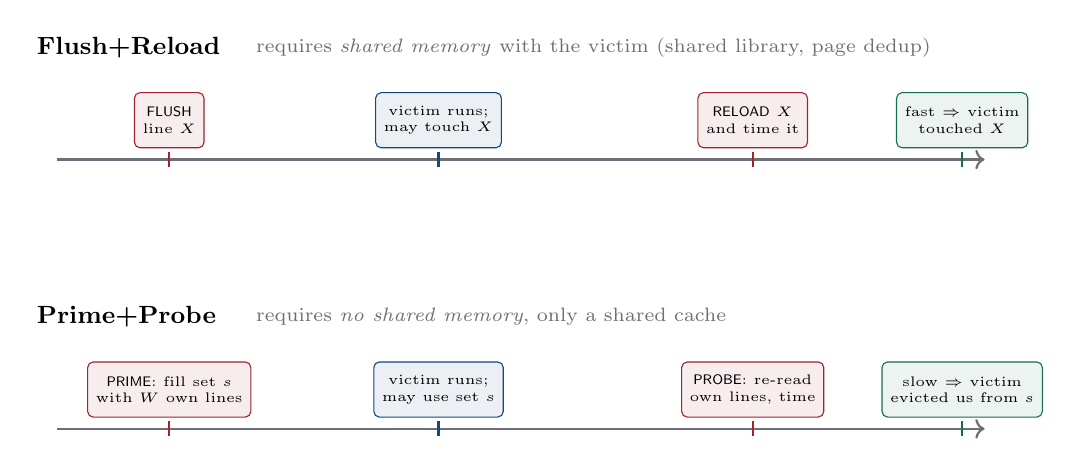
\begin{tikzpicture}[scale=0.95, every node/.style={font=\scriptsize}]
  % ---------- Flush+Reload ----------
  \node[anchor=west, font=\small\bfseries] at (-0.4,2.1) {Flush+Reload};
  \node[note, anchor=west] at (2.6,2.1) {requires \emph{shared memory} with the victim
       (shared library, page dedup)};
  \draw[->, thick, muted] (0,0.6) -- (12.4,0.6);
  \foreach \x/\lab/\c in {0.6/{\textsf{FLUSH}\\line $X$}/attack,
                          4.2/{victim runs;\\may touch $X$}/accent,
                          8.4/{\textsf{RELOAD} $X$\\and time it}/attack,
                          11.2/{fast $\Rightarrow$ victim\\touched $X$}/defense}
     {\node[draw=\c, fill=\c!8, rounded corners=2pt, minimum height=7mm, inner sep=3pt,
            align=center, font=\tiny, anchor=south] at (\x+0.9,0.75) {\lab};
      \draw[\c, thick] (\x+0.9,0.5) -- (\x+0.9,0.7);}
  % ---------- Prime+Probe ----------
  \node[anchor=west, font=\small\bfseries] at (-0.4,-1.5) {Prime+Probe};
  \node[note, anchor=west] at (2.6,-1.5) {requires \emph{no shared memory}, only a shared cache};
  \draw[->, thick, muted] (0,-3.0) -- (12.4,-3.0);
  \foreach \x/\lab/\c in {0.6/{\textsf{PRIME}: fill set $s$\\with $W$ own lines}/attack,
                          4.2/{victim runs;\\may use set $s$}/accent,
                          8.4/{\textsf{PROBE}: re-read\\own lines, time}/attack,
                          11.2/{slow $\Rightarrow$ victim\\evicted us from $s$}/defense}
     {\node[draw=\c, fill=\c!8, rounded corners=2pt, minimum height=7mm, inner sep=3pt,
            align=center, font=\tiny, anchor=south] at (\x+0.9,-2.85) {\lab};
      \draw[\c, thick] (\x+0.9,-3.1) -- (\x+0.9,-2.9);}
\end{tikzpicture}
\caption[Flush+Reload and Prime+Probe]{The two canonical cache measurement
primitives. Flush+Reload~\citep{yarom2014flushreload} is precise (line
granularity, low noise) but needs memory shared with the victim.
Prime+Probe~\citep{osvik2006cache,liu2015llc} needs no sharing at all and
therefore works across processes and across cores, at the cost of set-granular
resolution and more noise.}
\label{fig:primitives}
\end{figure}

\begin{table}[t]
\centering
\caption[Comparison of cache attack primitives]{The four principal cache
measurement primitives, with the weakest threat tier (\Cref{tab:threat}) at which
each is known to work. ``Shared memory'' means the attacker and victim map the
same physical page.}
\label{tab:primitives}
\footnotesize
\begin{tabularx}{\linewidth}{@{}p{2.3cm}p{1.5cm}p{2.4cm}X@{}}
\toprule
\textbf{Primitive} & \textbf{Tier} & \textbf{Requires} & \textbf{Characteristics} \\
\midrule
Evict+Time \newline \citep{osvik2006cache} & T2 &
Ability to trigger the victim &
Measures the victim's own run time after evicting a set. Coarse and noisy;
historically first. \\
\addlinespace
Prime+Probe \newline \citep{osvik2006cache,liu2015llc} & T3 &
Shared cache only &
Set granularity. Works cross-core on an inclusive LLC. Needs an eviction set,
whose construction is the main engineering cost. \\
\addlinespace
Flush+Reload \newline \citep{yarom2014flushreload} & T2/T3 &
Shared memory \emph{and} a flush instruction &
Line granularity, very low noise, high bandwidth. On RISC-V requires
\code{cbo.flush} (Zicbom) or an equivalent eviction. \\
\addlinespace
Flush+Flush \newline \citep{gruss2016flushflush} & T2/T3 &
Shared memory &
Times the \emph{flush} rather than the reload; leaves no cache footprint of its
own, so it evades detectors that watch for miss-rate anomalies. \\
\bottomrule
\end{tabularx}
\end{table}

\subsection{Prime+Probe in detail}

\Cref{alg:primeprobe} states the primitive precisely. The interesting part is
step~1: constructing an eviction set, a group of $W$ addresses that map to the
same cache set as the target.

\begin{algorithm}[t]
\caption{Prime+Probe on one cache set}
\label{alg:primeprobe}
\begin{algorithmic}[1]
\State $E \gets$ \Call{BuildEvictionSet}{$s$} \Comment{$|E| = W$, all mapping to set $s$}
\For{each measurement round}
  \State \textbf{prime:} access every line in $E$ \Comment{set $s$ now holds only attacker lines}
  \State \textbf{wait:} allow the victim to execute
  \State $t \gets$ \Call{TimedAccess}{$E$} \Comment{re-read the eviction set, timing it}
  \If{$t > \theta$}
     \State record ``victim used set $s$ in this round''
  \EndIf
\EndFor
\State aggregate rounds; apply majority vote to suppress noise
\end{algorithmic}
\end{algorithm}

For a virtually indexed L1 the index bits come from the page offset, so an\index{eviction set!construction}
eviction set is easy to construct. For a physically indexed LLC the index depends
on physical address bits the attacker cannot see, and on many designs the set is
further selected by a hash across slices. The standard solution is to use huge
pages to control more physical index bits, and then to reduce a large candidate
set to a minimal eviction set by an adaptive group-testing
procedure~\citep{liu2015llc}. On an open RISC-V platform the mapping is
documented in the RTL, which makes the construction dramatically easier, a
concrete instance of openness helping the analyst.

\subsection{What the measurement looks like}

\Cref{fig:histogram} shows the shape of the raw data: a bimodal distribution of
access times whose two modes correspond to hit and miss. Classification is a
threshold test, and the separation between modes is what makes the channel
reliable.

\begin{figure}[t]
\centering
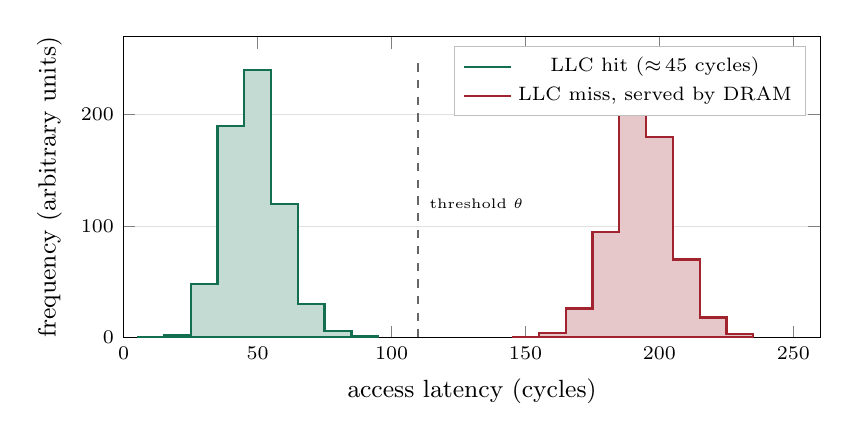
\begin{tikzpicture}
\begin{axis}[
  height=5.4cm, width=0.86\linewidth,
  xmin=0, xmax=260, ymin=0, ymax=270,
  xtick={0,50,100,150,200,250},
  xlabel={access latency (cycles)}, ylabel={frequency (arbitrary units)},
  ymajorgrids=true, grid style={draw=black!12},
  tick label style={font=\scriptsize}, label style={font=\small},
  legend style={font=\scriptsize, draw=black!25, at={(0.98,0.97)}, anchor=north east},
  ]
  \addplot[const plot, fill=defense!25, draw=defense, thick] coordinates {
    (5,0) (15,2) (25,48) (35,190) (45,240) (55,120) (65,30) (75,6) (85,1) (95,0)}
    \closedcycle;
  \addlegendentry{LLC hit ($\approx$\,45 cycles)}
  \addplot[const plot, fill=attack!25, draw=attack, thick] coordinates {
    (145,0) (155,4) (165,26) (175,95) (185,205) (195,180) (205,70) (215,18) (225,3) (235,0)}
    \closedcycle;
  \addlegendentry{LLC miss, served by DRAM}
  \draw[dashed, thick, black!60] (axis cs:110,0) -- (axis cs:110,250);
  \node[font=\tiny, anchor=west, fill=white, inner sep=1pt]
        at (axis cs:113,120) {threshold $\theta$};
\end{axis}
\end{tikzpicture}
\caption[Bimodal timing distribution]{The shape of a cache-timing measurement,
here for a last-level-cache probe: two well-separated modes, classified by a
single threshold. The modes sit at the LLC and DRAM latencies of
\Cref{fig:hierarchy}; probing L1 instead moves both modes down and widens their
separation in relative terms.
\textbf{Illustrative distributions, not measured data}: the author's measured
histograms for a RISC-V core are experiment~E1 of \Cref{ch:evalplan}. The point
of the figure is the \emph{separation}: classification error is small even for a
single measurement, and repetition drives it to nil.}
\label{fig:histogram}
\end{figure}

\section{Virtual memory and the translation path}

\SecRef{11.4} introduces virtual memory: \SecRef{11.4.3} develops paging, and
\SecRef{11.4.5} the memory management unit that caches recent translations in a\index{memory management unit (MMU)}
TLB. RISC-V uses a radix page table\index{paging!Sv39 and Sv48}
(Sv39, Sv48) walked in hardware~\citep{riscv-priv}.
\Cref{fig:sv39} shows the path and marks the three distinct structures that leak.

\begin{figure}[t]
\centering
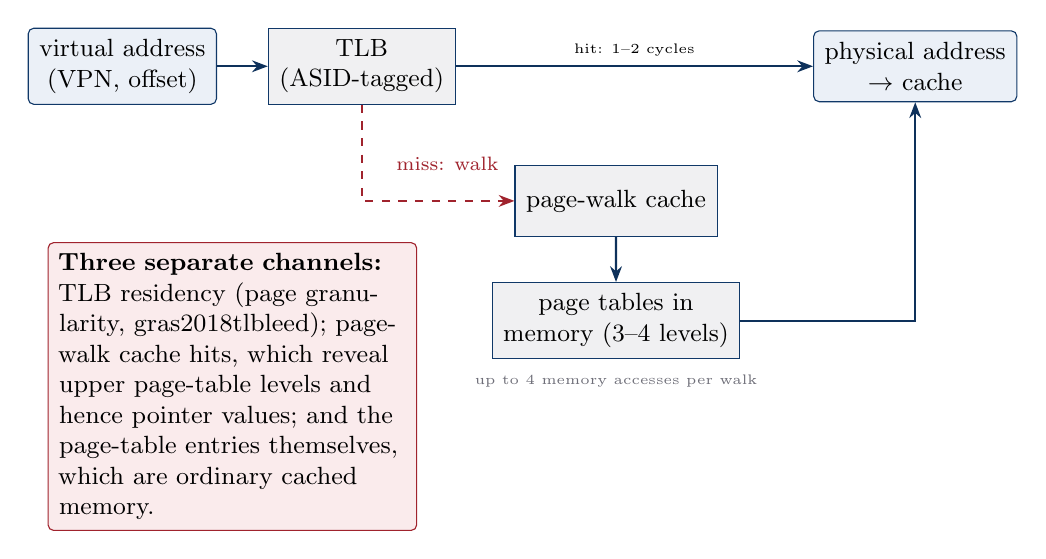
\begin{tikzpicture}[scale=0.95, every node/.style={font=\scriptsize}]
  \node[blk, minimum width=2.0cm, minimum height=0.9cm] (va) at (0,0) {virtual address\\(VPN, offset)};
  \node[memblk, minimum width=1.7cm, minimum height=0.9cm] (tlb) at (3.2,0) {TLB\\(ASID-tagged)};
  \node[blk, minimum width=1.9cm, minimum height=0.9cm] (pa) at (10.6,0) {physical address\\$\rightarrow$ cache};
  \node[memblk, minimum width=1.9cm, minimum height=0.9cm] (pwc) at (6.6,-1.8) {page-walk cache};
  \node[memblk, minimum width=1.9cm, minimum height=0.9cm] (pt) at (6.6,-3.4) {page tables in\\memory (3--4 levels)};

  \draw[sig] (va) -- (tlb);
  \draw[sig] (tlb) -- node[above, font=\tiny] {hit: 1--2 cycles} (pa);
  \draw[atksig] (tlb.south) |- (pwc.west);
  \node[note, anchor=north west, text=attack] at (3.6,-1.15) {miss: walk};
  \draw[sig] (pwc) -- (pt);
  \draw[sig] (pt.east) -| (pa.south);
  %% below the page-table box: the gap between it and the riser is too narrow
  \node[font=\tiny, anchor=north, text=muted] at (6.6,-4.0)
        {up to 4 memory accesses per walk};

  \node[atk, text width=4.4cm, align=left, anchor=north west] at (-1.0,-2.35)
    {\textbf{Three separate channels:} TLB residency (page granularity,
     \citep{gras2018tlbleed}); page-walk cache hits, which reveal upper
     page-table levels and hence pointer values; and the page-table entries
     themselves, which are ordinary cached memory.};
\end{tikzpicture}
\caption[Address translation and its channels]{The RISC-V Sv39 translation path
(\SecRef{11.4.3}, \SecRef{11.4.5}). Each acceleration structure on the path is a
separate transmitter. ASID tagging (\SecRef{11.4.6}) avoids TLB flushes on
context switch, a performance win that leaves another process's entries
resident and therefore contendable.}
\label{fig:sv39}
\end{figure}

The TLB channel is coarser than the cache channel (page rather than line\index{translation-lookaside buffer (TLB)!as a channel}
granularity) but it is harder to defend, for two reasons. First, the TLB is
small and fully associative, so a handful of accesses suffice to prime it.
Second, and more importantly, defences that flush or partition caches frequently
leave the TLB alone, because TLB pressure is a first-order performance concern.
That is the gap Gras \etal{} used to defeat cache-focused
protections using the TLB~\citep{gras2018tlbleed}.

\begin{takeaway}
The memory system offers not one channel but a family of them at different
granularities: line (L1/LLC), page (TLB), page-table level (walk cache), DRAM row\index{page-walk cache}
(row buffer), and the prefetcher's own stream tables, which Gruss
\etal~\citep{gruss2016prefetch} turned into an address-translation oracle. A
defence scoped to one member of the family does not constrain
the others. This ``whack-a-mole'' property is the strongest argument for the
principled, information-flow-based defences of \Cref{sec:taint} over
structure-specific patches.
\end{takeaway}

\begin{draftnote}
For v0.2 this chapter gains: (a) the eviction-set construction algorithm in full,
with its complexity analysis and a note on the RISC-V LLC slice hash;
(b) a quantitative bandwidth estimate for each primitive in
\Cref{tab:primitives}, tied to the leakage model of \Cref{sec:leakmodel};
(c) a worked AES T-table example showing precisely which key bits fall out of a
set-granular observation; and (d) the author's measured histograms replacing
\Cref{fig:histogram}. Target: +8 pages. This is the chapter that should grow the
most.
\end{draftnote}

\chapter{Multicore Systems: Sharing, Coherence and Cross-Domain Leakage}
\label{ch:multicore}

\begin{tocmapbox}
Background: textbook \SecRef{12.2} (software for multiprocessor systems,
including Amdahl's law in \SecRef{12.2.3}), \SecRef{12.3} (the design space of
multiprocessors), and \SecRef{12.4} (MIMD multiprocessors) with
\SecRef{12.4.1} (logical point of view), \SecRef{12.4.2} (coherence),
\SecRef{12.4.3} (memory consistency), \SecRef{12.4.4} (physical view of memory),
\SecRef{12.4.5} (shared caches), \SecRef{12.4.6} (coherent private caches) and
\SecRef{12.4.8} (multithreaded processors)~\citep{sarangi2025basic}.
\end{tocmapbox}

\section{What sharing adds}

Up to this point the attacker and the victim have taken turns on one core. A
multicore system removes that constraint: the attacker can run
\emph{simultaneously} with the victim, on a different core, and still share the
last-level cache, the interconnect, the memory controller and DRAM. This raises
the threat tier from T2 to T3 (\Cref{tab:threat}), which is the tier that matters
commercially, because it is the tier of cloud co-tenancy.

\Cref{fig:multicore} shows the organisation of \SecRef{12.3}--\SecRef{12.4.4} for
a four-core RISC-V system and marks what is private, what is shared, and what
leaks across which boundary.

\begin{figure}[t]
\centering
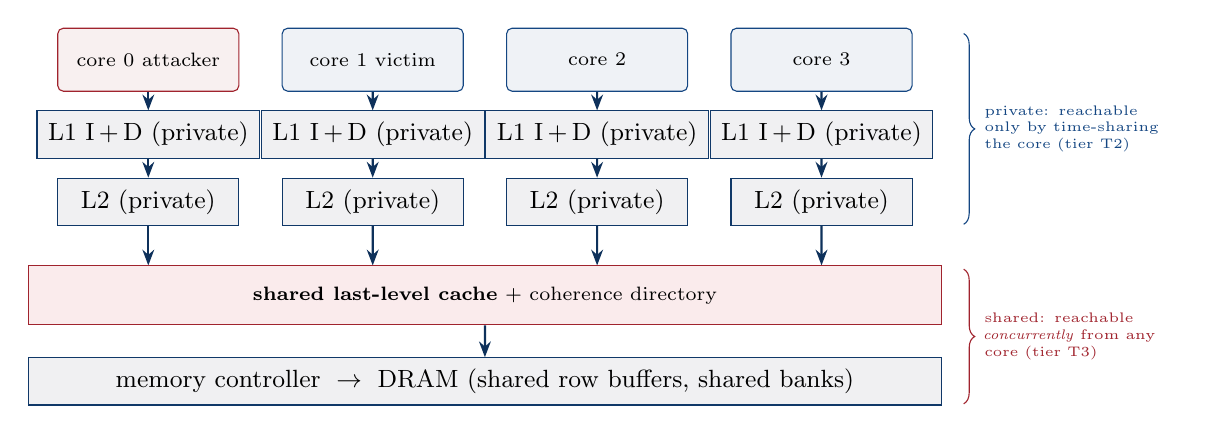
\begin{tikzpicture}[scale=0.95, every node/.style={font=\scriptsize}]
  \foreach \i/\x/\owner/\col in {0/0/attacker/attack, 1/3.0/victim/accent,
                                 2/6.0/{}/accent, 3/9.0/{}/accent}
  {
    \node[draw=\col, fill=\col!7, rounded corners=2pt, minimum width=2.3cm,
          minimum height=0.8cm] (c\i) at (\x,2.6) {core \i\ \owner};
    \node[memblk, minimum width=2.3cm, minimum height=0.6cm] (l1\i) at (\x,1.6) {L1 I\,+\,D (private)};
    \node[memblk, minimum width=2.3cm, minimum height=0.6cm] (l2\i) at (\x,0.7) {L2 (private)};
    \draw[sig] (c\i) -- (l1\i); \draw[sig] (l1\i) -- (l2\i);
    \draw[sig] (l2\i) -- (\x,-0.15);
  }
  \node[draw=attack, fill=attackfill, minimum width=11.6cm, minimum height=0.75cm]
       (llc) at (4.5,-0.55) {\textbf{shared last-level cache} + coherence directory};
  \node[memblk, minimum width=11.6cm, minimum height=0.6cm] (mc) at (4.5,-1.7)
       {memory controller \;$\rightarrow$\; DRAM (shared row buffers, shared banks)};
  \draw[sig] (llc) -- (mc);

  \draw[decorate, decoration={brace, amplitude=4pt}, accent]
       (10.9,2.95) -- (10.9,0.4)
       node[midway, right=4pt, align=left, text width=2.35cm, font=\tiny]
       {private: reachable only by time-sharing the core (tier T2)};
  \draw[decorate, decoration={brace, amplitude=4pt}, attack]
       (10.9,-0.2) -- (10.9,-2.0)
       node[midway, right=4pt, align=left, text width=2.35cm, font=\tiny, text=attack]
       {shared: reachable \emph{concurrently} from any core (tier T3)};
\end{tikzpicture}
\caption[Multicore sharing]{A four-core RISC-V system (\SecRef{12.4.4},
\SecRef{12.4.5}, \SecRef{12.4.6}). Private
caches require the attacker to time-share a core; the LLC, the directory, the
interconnect and DRAM are shared continuously. An \emph{inclusive} LLC couples
the two regions: evicting a line from the LLC forces its eviction from another
core's private L1, which is what makes cross-core Prime+Probe
practical~\citep{liu2015llc}.}
\label{fig:multicore}
\end{figure}

\section{Coherence as a channel}

\SecRef{12.4.2} develops cache coherence: the invariant that all cores observe a
single value for each memory location, maintained by a protocol such as MSI or\index{cache coherence!MESI protocol}
MESI, and \SecRef{12.4.6} applies it to coherent private caches. \Cref{fig:mesi} shows the states and the transitions that matter here.

\begin{figure}[t]
\centering
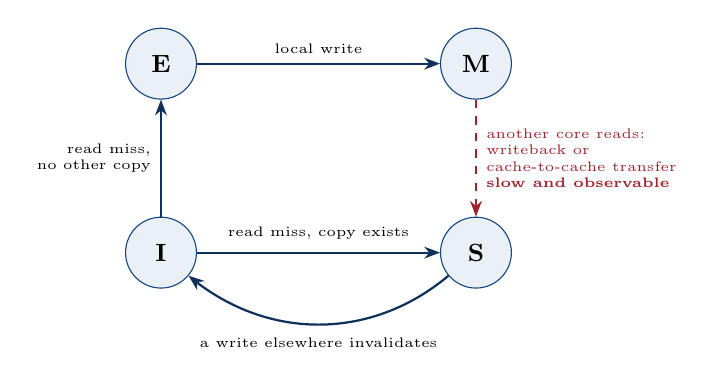
\begin{tikzpicture}[scale=1.0, every node/.style={font=\scriptsize},
                    st/.style={draw=accent, fill=lightfill, circle, minimum size=9mm,
                               font=\small\bfseries}]
  \node[st] (i) at (0,0)   {I};
  \node[st] (e) at (0,2.4) {E};
  \node[st] (m) at (4.0,2.4) {M};
  \node[st] (s) at (4.0,0) {S};
  \draw[sig] (i) -- node[left, font=\tiny, align=right]
        {read miss,\\no other copy} (e);
  \draw[sig] (e) -- node[above, font=\tiny] {local write} (m);
  \draw[atksig] (m) -- node[right, font=\tiny, align=left, text=attack]
        {another core reads:\\writeback or\\cache-to-cache transfer\\\textbf{slow and observable}} (s);
  %% bowed below so the label clears both state circles
  \draw[sig] (s) to[out=-140,in=-40] node[below=1pt, font=\tiny, pos=0.5]
        {a write elsewhere invalidates} (i);
  \draw[sig] (i) -- node[above=1pt, font=\tiny, pos=0.5]
        {read miss, copy exists} (s);
\end{tikzpicture}
\par\vspace{4pt}
\begin{tcolorbox}[enhanced, width=0.92\linewidth, colback=attackfill, colframe=attack,
  boxrule=0.4pt, arc=2pt, left=7pt, right=7pt, top=5pt, bottom=5pt, fontupper=\small]
\textbf{Why this is a channel.} Coherence transitions have different costs.
Reading a line that another core holds in M requires a writeback or a
cache-to-cache transfer and is measurably slower than reading a line in S. The
attacker therefore learns not only \emph{whether} the victim touched a line, but
\emph{whether it wrote to it}, a strictly stronger observation than the plain
cache-state channel of \Cref{ch:memsys}.
\end{tcolorbox}
\caption[MESI states and their timing]{The MESI coherence protocol
(\SecRef{12.4.2}, \SecRef{12.4.6}) and the transitions that create a channel. Coherence is a
correctness mechanism; the timing asymmetry between its transitions is an
unintended, and unavoidable, side effect.}
\label{fig:mesi}
\end{figure}

Two consequences follow.

\textbf{Coherence-based read/write discrimination.} Because a remote read of a
modified line costs more than a remote read of a shared line, an attacker with\index{cache coherence!read/write discrimination}
access to a shared line can distinguish victim \emph{reads} from victim
\emph{writes}. This extends the observation vocabulary beyond ``touched / not
touched''.

\textbf{Invalidation as a transmitter.} A write by one core invalidates copies
held by others. An attacker holding a copy of a shared line detects the\index{cache coherence!invalidation as transmitter}
invalidation as a subsequent miss, a channel that requires no eviction and
no capacity pressure at all.

\section{Memory consistency and fences}

\SecRef{12.4.3} covers memory consistency: the rules governing the order in
which one core's memory operations become visible to others\index{memory consistency!RVWMO}. RISC-V specifies
the RVWMO weak model with explicit \code{fence} instructions~\citep{riscv-unpriv}.

For this paper the relevant observation is a negative one, and it is a common
source of confusion: \textbf{a memory fence is an ordering instruction, not an\index{fence instruction!ordering versus erasure}
erasure instruction}. \code{fence} constrains \emph{when} operations become
visible; it does not remove cache lines, TLB entries or predictor state. Using
fences as a Spectre mitigation works only in the narrow sense that a
speculation barrier prevents later instructions from executing early: it
stops the transmitter from running, but it does not clean up after transmitters
that already ran. This distinction is what motivates the separate
\code{fence.t} proposal~\citep{wistoff2021fencet}, whose entire purpose is
erasure rather than ordering.

\section{Simultaneous multithreading}

Multithreaded processors are the subject of \SecRef{12.4.8}. When two threads
share one core's pipeline, they share the L1 caches, the TLB, the predictors, and\index{simultaneous multithreading (SMT)}
every functional unit and issue port. The result is the
tightest possible coupling: contention for a single execution port is observable\index{port contention}
at cycle granularity, and no cache-state change is required at all. Several
open RISC-V cores are single-threaded, which incidentally removes this attack
surface; it returns as soon as SMT is added for throughput.

\begin{takeaway}
Every sharing decision in \Cref{fig:multicore} is a performance decision that
also determines an attack surface, and the two are not separable. Inclusive LLCs
simplify coherence \emph{and} enable cross-core eviction. ASID-tagged TLBs avoid
flushes \emph{and} retain another domain's entries. SMT raises throughput
\emph{and} shares issue ports. There is no version of these choices that is fast
and non-shared.
\end{takeaway}

\section{Partitioning and colouring, viewed as defences}
\label{sec:partitioning}

The textbook's treatment of shared caches (\SecRef{12.4.5}) and coherent private
caches (\SecRef{12.4.6}) establishes \emph{why} cache resources are shared and
how coherence is maintained across them. Partitioning and colouring, by contrast,
are not textbook material: they come from the research literature, and they are
the oldest hardware defence against cache channels. This is the first point in
the paper where the argument leaves the prescribed text and relies on the
research sources instead. \Cref{fig:partition} contrasts the two mechanisms.

\begin{figure}[t]
\centering
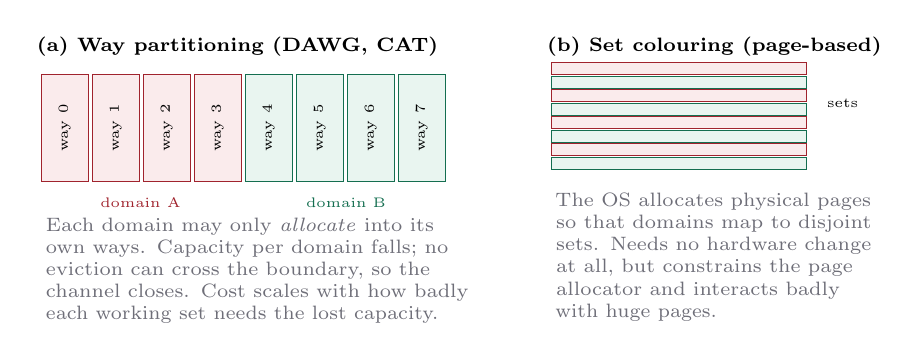
\begin{tikzpicture}[scale=0.9, every node/.style={font=\tiny}]
  % --- way partitioning ---
  \node[font=\scriptsize\bfseries, anchor=west] at (-0.2,3.1) {(a) Way partitioning (DAWG, CAT)};
  \foreach \w in {0,...,7}{
    \pgfmathsetmacro{\xx}{\w*0.72}
    \ifnum\w<4
      \draw[fill=attackfill, draw=attack] (\xx,1.2) rectangle ++(0.66,1.5);
    \else
      \draw[fill=defensefill, draw=defense] (\xx,1.2) rectangle ++(0.66,1.5);
    \fi
    \node[rotate=90] at (\xx+0.33,1.95) {way \w};}
  \node[anchor=north, text=attack] at (1.4,1.1) {domain A};
  \node[anchor=north, text=defense] at (4.3,1.1) {domain B};
  \node[note, anchor=north west, text width=5.4cm] at (0,0.75)
    {Each domain may only \emph{allocate} into its own ways. Capacity per domain
     falls; no eviction can cross the boundary, so the channel closes. Cost scales
     with how badly each working set needs the lost capacity.};

  % --- set partitioning / colouring ---
  \node[font=\scriptsize\bfseries, anchor=west] at (7.0,3.1) {(b) Set colouring (page-based)};
  \foreach \s in {0,...,7}{
    \pgfmathsetmacro{\yy}{2.7-\s*0.19}
    \ifodd\s
      \draw[fill=defensefill, draw=defense] (7.2,\yy) rectangle ++(3.6,0.17);
    \else
      \draw[fill=attackfill, draw=attack] (7.2,\yy) rectangle ++(3.6,0.17);
    \fi}
  \node[anchor=west] at (10.95,2.3) {sets};
  \node[note, anchor=north west, text width=4.0cm] at (7.2,1.1)
    {The OS allocates physical pages so that domains map to disjoint sets. Needs
     no hardware change at all, but constrains the page allocator and interacts
     badly with huge pages.};
\end{tikzpicture}
\caption[Two partitioning mechanisms]{Way partitioning versus set colouring,
applied to the shared caches of \SecRef{12.4.5}. Both enforce non-interference by
construction rather than by obscurity, which is why they give the strongest guarantees of any defence class
in \Cref{ch:defenses}, and why both pay for it in effective capacity.}
\label{fig:partition}
\end{figure}

The two mechanisms fail differently, which matters when choosing between them.
Way partitioning caps the number of protected domains at the associativity\index{cache partitioning!way partitioning}
(eight ways means at most eight isolated domains) and requires hardware support;
DAWG~\citep{kiriansky2018dawg} is the fully worked hardware design, and Intel's
Cache Allocation Technology is the deployed commercial approximation, used as a
security mechanism by CATalyst~\citep{liu2016catalyst}. Set colouring requires
no hardware change but takes control of physical page allocation away from the\index{page colouring}
memory manager, and is defeated by any mechanism that changes the
virtual-to-set mapping, including huge pages.

\begin{draftnote}
For v0.2 this chapter gains: (a) the directory-based coherence channel described
quantitatively, with the transition-cost table that \Cref{ch:tradeoffs} needs;
(b) a treatment of interconnect and memory-controller contention channels, which
are the ones that survive every cache-level defence; and (c) a concrete mapping
onto the coherence implementation of an open RISC-V uncore (TileLink), so the
discussion is tied to inspectable RTL. Target: +5 pages.
\end{draftnote}

\chapter{Transient Execution Attacks}
\label{ch:transient}

This chapter synthesises the preceding four. It has no single textbook
counterpart (transient-execution attacks post-date most textbook treatments of
pipelining) but it is built entirely from material developed in
\Cref{ch:pipeline} (speculation, squashing, precise exceptions, the execution
window) and \Cref{ch:memsys} (the cache as a receiver).

\section{Anatomy}

Every transient-execution attack has the same four phases, shown in\index{transient execution!four phases}
\Cref{fig:anatomy}. The phase decomposition used here follows the
systematisation of Canella \etal~\citep{canella2019systematic}, whose
classification of the attack space by mis-speculation source and by transmitter
remains the standard organisation of the field. Naming them separately is useful because defences attack
different phases, and two defences that block different phases compose while two
that block the same phase do not.

\begin{figure}[t]
\centering
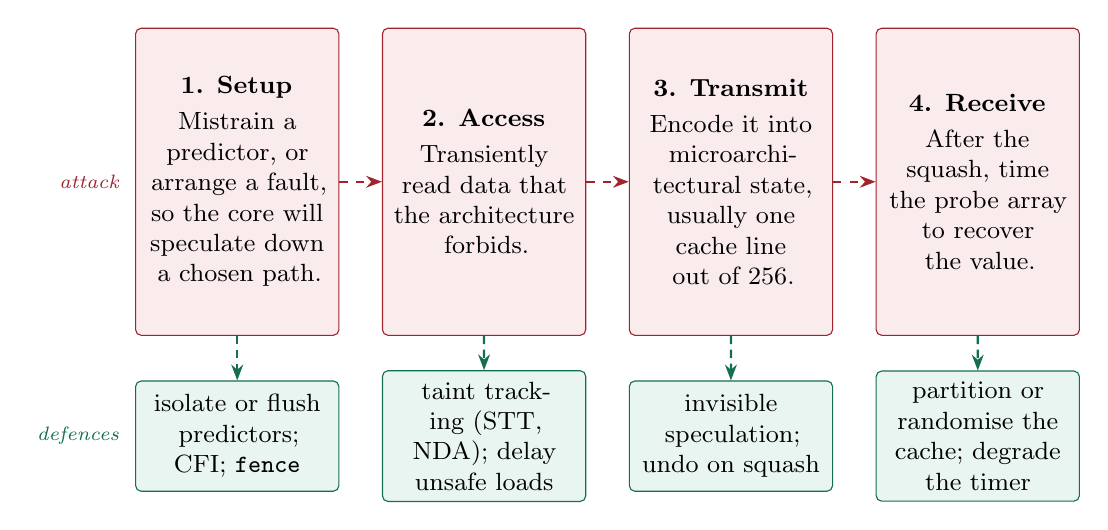
\begin{tikzpicture}[scale=0.95, every node/.style={font=\scriptsize}]
  \node[atk, minimum width=2.5cm, minimum height=3.9cm, text width=2.3cm] (p1) at (0,0)
       {\textbf{1. Setup}\\[2pt] Mistrain a predictor, or arrange a fault, so the core
        will speculate down a chosen path.};
  \node[atk, minimum width=2.5cm, minimum height=3.9cm, text width=2.3cm] (p2) at (3.3,0)
       {\textbf{2. Access}\\[2pt] Transiently read data that the architecture
        forbids.};
  \node[atk, minimum width=2.5cm, minimum height=3.9cm, text width=2.3cm] (p3) at (6.6,0)
       {\textbf{3. Transmit}\\[2pt] Encode it into \uarchadj{} state, usually one
        cache line out of 256.};
  \node[atk, minimum width=2.5cm, minimum height=3.9cm, text width=2.3cm] (p4) at (9.9,0)
       {\textbf{4. Receive}\\[2pt] After the squash, time the probe array to
        recover the value.};
  \foreach \a/\b in {p1/p2, p2/p3, p3/p4} {\draw[atksig] (\a) -- (\b);}

  \node[def, minimum width=2.5cm, text width=2.3cm, minimum height=1.4cm] (d1) at (0,-3.4)
       {isolate or flush predictors; CFI; \code{fence}};
  \node[def, minimum width=2.5cm, text width=2.3cm, minimum height=1.4cm] (d2) at (3.3,-3.4)
       {taint tracking (STT, NDA); delay unsafe loads};
  \node[def, minimum width=2.5cm, text width=2.3cm, minimum height=1.4cm] (d3) at (6.6,-3.4)
       {invisible speculation; undo on squash};
  \node[def, minimum width=2.5cm, text width=2.3cm, minimum height=1.4cm] (d4) at (9.9,-3.4)
       {partition or randomise the cache; degrade the timer};
  \foreach \a/\b in {p1/d1, p2/d2, p3/d3, p4/d4} {\draw[defsig, densely dashed] (\a) -- (\b);}
  \node[anchor=east, font=\scriptsize\itshape, text=attack]  at (-1.45,0)    {attack};
  \node[anchor=east, font=\scriptsize\itshape, text=defense] at (-1.45,-3.4) {defences};
\end{tikzpicture}
\caption[Anatomy of a transient-execution attack]{The four phases of a
transient-execution attack, and the defence class that targets each. The
taxonomy of \Cref{ch:defenses} is organised by which phase a mechanism attacks,
because that determines what it can and cannot cover.}
\label{fig:anatomy}
\end{figure}

\section{Spectre-v1: bounds-check bypass}

\Cref{lst:spectre1} is the canonical gadget~\citep{kocher2019spectre}. The bounds
check is correct: architecturally, \code{x} is never out of range. But if the
attacker first calls the function many times with in-range \code{x}, the
direction predictor learns ``taken'', and on a subsequent out-of-range call the\index{Spectre!v1, bounds-check bypass}
core speculatively executes the body before the comparison resolves.

\begin{lstlisting}[language=C, caption={The Spectre-v1 gadget in C. Phases 1--3
of \Cref{fig:anatomy} all occur inside these three lines; phase 4 happens in the
attacker's own code afterwards.}, label={lst:spectre1}]
if (x < array1_size) {          /* mistrained: predicted TAKEN  */
    uint8_t v = array1[x];      /* transient out-of-bounds read */
    temp &= array2[v * 512];    /* transmit: 1 line out of 256  */
}
\end{lstlisting}

Compiled for RV64GC the same gadget is \Cref{lst:spectre1rv}. Nothing in the
RISC-V encoding, the privilege model or the memory model prohibits any
instruction here; the sequence is architecturally impeccable and
\uarchadv{} catastrophic.

\begin{lstlisting}[language=riscv, caption={The same gadget in RISC-V assembly.
The branch at line~2 is the one that is mistrained; lines 3--9 are the transient
window; line~9 is the transmitter.}, label={lst:spectre1rv}]
  ld    t0, array1_size      # bound
  bgeu  a0, t0, .Lskip       # mistrained: predicted NOT taken
  la    t1, array1
  add   t1, t1, a0           # transiently computes an out-of-bounds address
  lbu   t2, 0(t1)            # transient read of forbidden data -> t2
  slli  t2, t2, 9            # scale by 512 bytes
  la    t3, array2
  add   t3, t3, t2
  lbu   t4, 0(t3)            # TRANSMIT: allocates one of 256 cache lines
.Lskip:
  ret                        # branch resolves; everything above is squashed
\end{lstlisting}

\begin{takeaway}
Spectre-v1 needs no privilege escalation, no fault and no architectural bug, only
a mispredicted branch and a cache. Nothing in microcode can take those away,
and every defence in \Cref{ch:defenses} costs performance for the same reason:
the mechanism being exploited \emph{is} the performance mechanism.
\end{takeaway}

\section{The variant family}

\Cref{tab:variants} organises the main variants by the \uarchadj{} mechanism they
exploit, and (the column that matters for a RISC-V paper) what is actually
known about their applicability to open RISC-V cores.

\begin{table}[t]
\centering
\caption[Transient-execution variants]{The principal transient-execution
variants, the mechanism each exploits, and the state of the evidence on RISC-V.
The last column deliberately distinguishes \emph{demonstrated on RISC-V} from
\emph{expected by construction}; conflating the two is the most common error in
survey treatments of this topic.}
\label{tab:variants}
\footnotesize
\begin{tabularx}{\linewidth}{@{}p{2.6cm}p{3.4cm}X@{}}
\toprule
\textbf{Variant} & \textbf{Mechanism} & \textbf{RISC-V status} \\
\midrule
Spectre-v1 \newline (bounds-check bypass) \citep{kocher2019spectre} &
Mistrained direction predictor; transient out-of-bounds load &
\textbf{Demonstrated} on the open BOOM out-of-order core, with mitigations
evaluated on the same RTL~\citep{gonzalez2019replicating}. Applies to any core
with a direction predictor and a speculation window. \\
\addlinespace
Spectre-v2 \newline (branch target injection) \citep{kocher2019spectre} &
Attacker-poisoned BTB or indirect predictor redirects victim speculation to a
chosen gadget &
Expected on any core with a shared, untagged BTB. Branch-history
injection~\citep{barberis2022bhi} shows that partial isolation is insufficient
when history is shared. \\
\addlinespace
Spectre-v4 \newline (speculative store bypass) &
A load speculatively bypasses an older store whose address is not yet known,
reading stale data &
Applies to any core with speculative store-to-load forwarding disambiguation.
Cores without speculative disambiguation are immune \emph{by construction}, an
important architectural distinction. \\
\addlinespace
Spectre-RSB / Retbleed \citep{wikner2022retbleed} &
Return-address-stack underflow or poisoning redirects speculative returns &
Applies to any core with a RAS that falls back to the BTB on underflow. \\
\addlinespace
Meltdown-type \citep{lipp2018meltdown,vanbulck2018foreshadow} &
A faulting load's data is forwarded to dependent instructions \emph{before} the
permission check retires &
Depends on whether the implementation forwards data past a failed PMP or page
permission check. This is an \textbf{implementation choice, not an ISA
property}: a core that checks before forwarding is immune. \\
\addlinespace
MDS-type \citep{vanschaik2019ridl,schwarz2019zombieload} &
Stale data sampled from line-fill buffers, store buffers or load ports &
Requires the specific buffer structures involved; not demonstrated on published
open RISC-V cores. Listed here for completeness of the taxonomy. \\
\bottomrule
\end{tabularx}
\end{table}

Two entries in \Cref{tab:variants} deserve emphasis because they show the
argument of \Cref{ch:isa} paying off.

\textbf{Meltdown is an implementation choice.} Whether a faulting load forwards
its data to dependent instructions before the fault is architecturally raised is\index{Meltdown}
not specified by RISC-V. An implementation that resolves the PMP or page
permission check before forwarding is immune to Meltdown-type attacks and pays
for it only in the latency of the check. Here the architecture/organization
distinction that opens the textbook becomes operational: two conforming
implementations, one vulnerable and one not.

\textbf{Spectre-v4 is a structural choice.} A core that does not speculate on
store-to-load dependences cannot exhibit speculative store bypass. Simpler cores\index{Spectre!v4, speculative store bypass}
get this security property for free, and pay for it in performance.

\section{Why the attacks reached RISC-V}

Gonzalez \etal~\citep{gonzalez2019replicating} replicated Spectre-v1 and related
variants on BOOM and evaluated mitigations in RTL\index{Spectre!replication on RISC-V}. Their result matters for two
separate reasons. The negative one is that RISC-V provides no inherent immunity:
the attacks follow from out-of-order speculation, not from any x86 peculiarity.
The positive one is methodological: because the RTL is open, the work could
identify exactly which structure carried the leak and measure the cost of
changing it, an end-to-end chain unavailable on closed silicon.

The corollary for core selection is direct. In-order cores such as
Rocket~\citep{asanovic2016rocket} have a very small speculation window and are
correspondingly hard to exploit with the transient-execution family, though they
remain fully exposed to the classical cache side channels of \Cref{ch:memsys}.
Out-of-order cores such as BOOM~\citep{zhao2020sonicboom} have windows large
enough to run a complete access-and-transmit sequence transiently. Security is
therefore a factor in the in-order/out-of-order decision, alongside performance,
area and power, which is the argument \Cref{ch:tradeoffs} makes quantitative.

\section{Attacks on the defences}

A survey that stops at the defence list would misrepresent the field. Two
results are essential context for \Cref{ch:defenses}:

\textbf{Speculative interference}~\citep{behnia2021interference} showed that
schemes which hide the \emph{cache-state} effects of speculation are still
observable, because transient instructions perturb the \emph{timing} of
non-transient ones through contention for shared resources. Making speculation\index{speculative interference attacks}
invisible in the cache hierarchy is therefore not sufficient by itself.

\textbf{Attacks on randomised caches}~\citep{qureshi2019ceasers} showed that
address-encryption schemes must re-key faster than an attacker can construct an
eviction set, turning a static design into a rate race and forcing the successor
designs discussed in \Cref{sec:randomisation}.

\begin{draftnote}
For v0.2: add (a) a phase-by-phase mapping from each variant in
\Cref{tab:variants} onto \Cref{fig:anatomy}, so that the defence coverage
argument of \Cref{ch:defenses} can be stated as a matrix rather than in prose;
(b) a measured or simulated speculation-window figure for BOOM, showing how many
transient instructions actually execute as a function of ROB size; this is
experiment~E3 in \Cref{ch:evalplan}; and (c) a short treatment of speculative
interference with a worked example. Target: +6 pages.
\end{draftnote}

\chapter{Defences: A Taxonomy with Residual Risk}
\label{ch:defenses}

\section{Organising the design space}

The defence literature is large and the mechanisms are heterogeneous, so a\index{defences!taxonomy}
taxonomy is necessary before comparison is possible. \Cref{fig:taxonomy}
organises the space by \emph{what the mechanism does to the channel} rather than
by publication venue or date, which is the organisation that makes coverage gaps
visible.

\begin{figure}[t]
\centering
\resizebox{\linewidth}{!}{%
\begin{forest}
  for tree={
    grow'=east, parent anchor=east, child anchor=west,
    edge={draw=muted, -{Stealth[length=1.6mm]}},
    l sep=6mm, s sep=1.6mm, anchor=west, align=left,
    font=\scriptsize,
    edge path={\noexpand\path[\forestoption{edge}]
      (!u.parent anchor) -- +(4mm,0) |- (.child anchor)\forestoption{edge label};},
  }
  [{\textbf{Defences against}\\\textbf{\uarchadj{} leakage}}, draw=accent, fill=lightfill,
    rounded corners, inner sep=3pt
    [{\textbf{Isolate}}\\{remove the sharing}, draw=defense, fill=defensefill, rounded corners, inner sep=2.5pt
      [{way partitioning (DAWG, CAT)}]
      [{set colouring / page colouring}]
      [{temporal flushing (\code{fence.t})}]
    ]
    [{\textbf{Obscure}}\\{keep sharing, break the mapping}, draw=defense, fill=defensefill, rounded corners, inner sep=2.5pt
      [{address randomisation (CEASER, ScatterCache)}]
      [{fully-associative emulation (Mirage)}]
      [{random or non-monopolisable replacement}]
    ]
    [{\textbf{Hide or undo}}\\{allow speculation, remove its trace}, draw=defense, fill=defensefill, rounded corners, inner sep=2.5pt
      [{invisible speculation (InvisiSpec, SafeSpec)}]
      [{rollback on squash (CleanupSpec)}]
      [{shadow structures (MuonTrap, GhostMinion)}]
    ]
    [{\textbf{Restrict}}\\{do not speculate on secrets}, draw=defense, fill=defensefill, rounded corners, inner sep=2.5pt
      [{taint tracking (STT, SPT, NDA)}]
      [{delay-on-miss / selective delay}]
      [{software: SLH, retpoline, fences}]
    ]
    [{\textbf{Contain}}\\{bound the damage architecturally}, draw=defense, fill=defensefill, rounded corners, inner sep=2.5pt
      [{PMP, enclaves (Sanctum, Keystone, MI6)}]
      [{CFI (\code{Zicfilp}, \code{Zicfiss})}]
      [{constant-time guarantees (\code{Zkt})}]
    ]
  ]
\end{forest}%
}
\caption[Defence taxonomy]{Taxonomy of defences by the operation each performs on
the channel, indexed against the attack phases of \Cref{fig:anatomy}:
\emph{isolate} and \emph{obscure} both attack the receiver by different means,
\emph{hide or undo} attacks the transmitter, \emph{restrict} attacks the access,
and \emph{contain} bounds what a successful attack yields. The mapping is not
one-to-one, and the two branches that share the receiver phase are the reason
\Cref{sec:incomparable} insists that a lower overhead may reflect a weaker
promise rather than a better design.}
\label{fig:taxonomy}
\end{figure}

\section{Isolation: partitioning and flushing}

Partitioning was introduced in \Cref{sec:partitioning} as an application of
cache colouring from \SecRef{12.4}. Its distinguishing property among all
defence classes is that it provides \emph{non-interference by construction}: if
two domains cannot allocate into the same cache resource, then no allocation by\index{non-interference}
one can be observed by the other, and the argument requires no assumption about
attacker cleverness. DAWG~\citep{kiriansky2018dawg} extends way partitioning to
cover metadata and coherence as well as data, closing the gaps that made naive\index{DAWG}
way partitioning incomplete.

Temporal isolation is the dual approach: instead of dividing the cache in space,
divide it in time and erase between slices\index{fence.t (temporal fence)}. \code{fence.t} on
CVA6~\citep{wistoff2021fencet} flushes \uarchadj{} state at a context switch and
normalises the timing of the switch itself, so that neither the residue nor the
duration of the flush leaks. The cost model is \Cref{eq:amat}: every flush
converts a warm cache into a cold one, so the penalty scales with the\index{flushing!cost at context switch}
context-switch rate and the working-set size, and is close to zero for
long-running compute-bound threads.

\begin{takeaway}
Isolation defences are the only class whose security argument is structural
rather than statistical. They are the natural choice for enclaves and real-time
systems for that reason, and a poor fit for general-purpose sharing for the same
one:
they charge the full cost of isolation to every workload, including the vast
majority that has no secret to protect.
\end{takeaway}

\section{Obscuring: randomised caches}
\label{sec:randomisation}

If an attacker cannot determine which addresses collide in a set, eviction sets\index{cache!randomisation}
cannot be constructed and Prime+Probe fails. The idea is older than the modern
designs: Wang and Lee's partition-locked and random-permutation
caches~\citep{wang2007newcache} proposed both locking lines against eviction and
randomising the address-to-set mapping, and non-monopolisable
caches~\citep{domnitser2012nonmono} showed that merely preventing one thread from
occupying a whole set already raises the attacker's cost substantially, at very
low hardware complexity. CEASER~\citep{qureshi2018ceaser}
encrypts the address before indexing, so the mapping from address to set is a\index{CEASER}
keyed permutation; ScatterCache~\citep{werner2019scattercache} goes further and
gives each security domain a different mapping, so that collisions are not merely\index{ScatterCache}
unknown but domain-specific.

The critical parameter is the \emph{re-keying rate}. An attacker can still
discover an eviction set empirically, given enough time; the design must change\index{re-keying rate}
the key faster than that discovery completes. Qureshi's own follow-up showed that
the original parameters were insufficient against faster eviction-set
construction, and raised the re-keying rate
accordingly~\citep{qureshi2019ceasers}. Mirage~\citep{saileshwar2021mirage} takes
a different route, using a pointer-based indirection to emulate full\index{Mirage}
associativity so that conflict-based eviction becomes statistically negligible
rather than merely obscured.

This class shows a general pattern: \textbf{defences
whose security rests on the attacker's cost rather than on a structural
impossibility have a parameter that must be tuned against the best known attack,
and therefore need revisiting whenever the attack improves.}

\section{Hiding and undoing speculative effects}

InvisiSpec~\citep{yan2018invisispec} buffers speculative loads in a speculative
buffer and only makes them visible in the cache hierarchy when they become\index{invisible speculation!InvisiSpec}
non-speculative, restoring the cache to the state it would have had without
speculation. SafeSpec~\citep{khasawneh2019safespec} uses shadow structures with
the same intent. CleanupSpec~\citep{saileshwar2019cleanupspec} inverts the
approach: allow speculation to modify the cache, and \emph{undo} the changes on a
squash, which is cheaper on average because most speculation is correct.\index{CleanupSpec}
MuonTrap~\citep{ainsworth2020muontrap} confines speculative state to a small
filter cache that is cleared at domain boundaries, and\index{MuonTrap}
GhostMinion~\citep{ainsworth2021ghostminion} adds a strict ordering discipline
designed to close the timing paths that speculative interference
exploits~\citep{behnia2021interference}.

The residual risk in this class is the one
\citet{behnia2021interference} identified: hiding cache-state changes does not
hide the \emph{contention} that transient instructions cause for ports,
bandwidth, MSHRs and queue slots. Any comparison table that lists these schemes
as ``blocks Spectre'' without that qualification is misleading, and
\Cref{tab:defenses} carries an explicit residual-risk column to avoid it.

\section{Restricting speculation: information-flow tracking}
\label{sec:taint}

The most principled class taints speculatively accessed data and forbids\index{information-flow tracking}
instructions that would transmit it. Speculative Taint Tracking
(STT)~\citep{yu2019stt} formalises \emph{when} data becomes safe (at the point
where the instruction that produced it is no longer squashable) and blocks\index{speculative taint tracking (STT)}
only transmitters that would act on tainted data before that point.
NDA~\citep{weisse2019nda} restricts the propagation of data from unresolved
instructions more conservatively. Speculative Privacy Tracking
(SPT)~\citep{choudhary2021spt} reduces the cost by observing that many
speculative values are not secret and need not be protected at all.\index{speculative privacy tracking (SPT)}
Sakalis \etal~\citep{sakalis2019delay} take a simpler route: delay loads that
miss in the L1 until they are non-speculative, and recover some of the lost\index{delay-on-miss}
performance with value prediction.

This class is attractive because its security argument is about
\emph{information} rather than about a particular structure, so it does not have
the whack-a-mole property noted in \Cref{ch:memsys}. Its costs are the
complexity of the tracking logic and a performance loss that depends heavily on
how aggressively ``safe'' is defined.

\section{Architectural containment in RISC-V}

RISC-V contributes several mechanisms that limit the \emph{consequences} of
leakage rather than the leakage itself. PMP and its enhanced variant restrict\index{physical memory protection (PMP)}
physical memory access per privilege level~\citep{riscv-priv}.
Sanctum~\citep{costan2016sanctum} showed that strong software isolation,
including protection against page-table and cache side channels, is achievable\index{Sanctum}
with minimal hardware extensions to a RISC-V core;
MI6~\citep{bourgeat2019mi6} extended enclave protection to a speculative
out-of-order core, which is the hard case; and Keystone~\citep{lee2020keystone}
provides an open, configurable TEE framework built on those foundations.\index{Keystone}
The \code{Zkt} extension~\citep{riscv-crypto} makes a narrow but genuinely
architectural promise of data-independent latency for listed instructions\index{Zkt extension!data-independent latency}, and
control-flow integrity via landing pads and shadow
stacks~\citep{riscv-cfi} raises the cost of assembling gadget chains, while\index{control-flow integrity (CFI)}
not, as noted in \Cref{tab:extensions}, constraining \emph{speculative} control
flow. A more radical containment approach replaces pointers with hardware\index{CHERI}
capabilities: CHERI~\citep{watson2015cheri} enforces bounds and permissions in
the hardware itself, which bounds what a transient access can reach even when
the speculation cannot be prevented.

\section{Software mitigations}

Software mitigations deserve a place in the taxonomy because they are what is
actually deployed while hardware catches up. Speculative load
hardening~\citep{carruth2018slh} masks addresses with a predicate derived from
the branch condition, so that a mis-speculated load reads a safe address;\index{speculative load hardening (SLH)}
retpolines~\citep{turner2018retpoline} replace indirect branches with a
construct that steers speculation to a benign target; and explicit fences before\index{retpoline}
sensitive loads stop the speculation window from opening at all. All three
increase $N_{\text{inst}}$ in \Cref{eq:iron}, and all three depend on the
compiler correctly identifying every vulnerable site, a static-analysis
problem with no complete solution.

\section{Comparison}

\Cref{tab:defenses} is the synthesis. The residual-risk column is the
contribution of this paper's treatment: it is the column most often omitted, and\index{residual risk}
the one a system designer most needs.

\begin{table}[p]
\centering
\caption[Comparison of defence mechanisms]{Comparison of representative
defences. Overheads are \textbf{as reported by the original authors}, on their
own baselines and benchmark suites; they are \emph{not} directly comparable with
one another, and \Cref{ch:tradeoffs} explains why. Verifying a subset of these
numbers on a common RISC-V platform is the purpose of the evaluation plan in
\Cref{ch:evalplan}.}
\label{tab:defenses}
\scriptsize
\begin{tabularx}{\linewidth}{@{}p{2.4cm}p{1.5cm}p{2.6cm}X@{}}
\toprule
\textbf{Mechanism} & \textbf{Class} & \textbf{Reported cost} & \textbf{Covers / residual risk} \\
\midrule
DAWG \citep{kiriansky2018dawg} & Isolate & Low for fitting working sets; grows at the capacity cliff &
Covers cache-based channels between partitioned domains. Residual: number of
domains capped by associativity; TLB and predictors untouched. \\
\addlinespace
Page colouring & Isolate & Depends on capacity loss; no hardware cost &
Covers set-conflict channels. Residual: defeated by huge pages; constrains the
page allocator; nothing outside the cache. \\
\addlinespace
\code{fence.t} \citep{wistoff2021fencet} & Isolate & Scales with context-switch rate &
Covers cross-context residue in flushed structures, with normalised switch
timing. Residual: nothing within a time slice; cost grows with state flushed. \\
\addlinespace
CEASER \citep{qureshi2018ceaser}, ScatterCache \citep{werner2019scattercache} & Obscure &
Small latency and energy addition for encryption &
Covers conflict-based eviction-set construction. Residual: security is a rate
race against eviction-set discovery~\citep{qureshi2019ceasers}; shared-memory
Flush+Reload unaffected. \\
\addlinespace
Mirage \citep{saileshwar2021mirage} & Obscure & Modest area and latency for indirection &
Makes set conflicts statistically negligible. Residual: does not address
occupancy or shared-line channels. \\
\addlinespace
InvisiSpec \citep{yan2018invisispec}, SafeSpec \citep{khasawneh2019safespec} & Hide &
Moderate slowdown; extra buffering &
Covers cache-state traces of transient loads. Residual: speculative
interference~\citep{behnia2021interference}; non-cache structures. \\
\addlinespace
CleanupSpec \citep{saileshwar2019cleanupspec} & Undo & Lower than hiding on average &
Covers cache traces via rollback. Residual: rollback itself is observable in
some designs; coherence effects are hard to undo. \\
\addlinespace
MuonTrap \citep{ainsworth2020muontrap}, GhostMinion \citep{ainsworth2021ghostminion} & Hide &
Low reported slowdown &
Confines speculative state; GhostMinion explicitly targets interference-style
timing paths. Residual: added structures and their own timing behaviour. \\
\addlinespace
STT \citep{yu2019stt}, SPT \citep{choudhary2021spt} & Restrict &
Moderate; SPT reduces STT's cost &
Principled: blocks transmission of speculatively accessed secrets, structure
independent. Residual: definition of ``safe'' bounds the guarantee; tracking
logic complexity. \\
\addlinespace
NDA \citep{weisse2019nda} & Restrict & Higher, varies with variant &
Broad coverage by restricting propagation from unresolved instructions.
Residual: cost rises steeply for the strictest configurations. \\
\addlinespace
Delay-on-miss \citep{sakalis2019delay} & Restrict & Substantially reduced by value prediction &
Covers speculative loads that miss. Residual: L1 hits still speculate; value
prediction adds its own structures. \\
\addlinespace
SLH \citep{carruth2018slh}, retpoline \citep{turner2018retpoline} & Restrict (SW) &
Instruction-count overhead; no hardware change &
Deployable today. Residual: depends on the compiler finding every gadget; does
not protect non-recompiled code. \\
\addlinespace
Sanctum \citep{costan2016sanctum}, MI6 \citep{bourgeat2019mi6}, Keystone \citep{lee2020keystone} &
Contain & Enclave entry/exit cost &
Strong isolation for enclave workloads on RISC-V. Residual: protects enclaves,
not general multi-tenant sharing. \\
\bottomrule
\end{tabularx}
\end{table}

\begin{draftnote}
For v0.2: (a) replace the qualitative ``reported cost'' column with numeric
values and, for each, the benchmark suite and baseline configuration used, so
that the incomparability is documented rather than merely asserted; (b) add a
coverage matrix of defence $\times$ attack-phase (\Cref{fig:anatomy}) showing
which combinations compose; and (c) add a paragraph on formal verification of
these mechanisms and on automated exploit synthesis
(CheckMate~\citep{trippel2018checkmate}) and cache-vulnerability
benchmarking~\citep{deng2020benchmark}. Target: +7 pages.
\end{draftnote}

\chapter{What Security Costs: Performance, Power and Area}
\label{ch:tradeoffs}

\begin{tocmapbox}
Background: textbook \SecRef{10.9.3} (performance metrics) and \SecRef{10.10}
(power and temperature issues), applied here to the pricing of security
mechanisms; \SecRef{11.3} (the memory-system model) supplies
\Cref{eq:amat}~\citep{sarangi2025basic}.
\end{tocmapbox}

\section{Why a whole chapter}

A defence that closes a channel is an engineering result only if its cost is
known. This chapter therefore does three things: it states honestly why the
published numbers cannot simply be tabulated against one another; it collates
them anyway, with their provenance attached; and it defines the common-footing
methodology that \Cref{ch:evalplan} will use to produce numbers that \emph{are}
comparable.

\section{Why published overheads are not comparable}
\label{sec:incomparable}

Four differences make direct comparison invalid, and all four are routinely\index{overheads!incomparability of published}
ignored:

\begin{enumerate}[leftmargin=1.8em]
  \item \textbf{Different baselines.} A 10\,\% slowdown against an aggressive
        8-wide out-of-order baseline and a 10\,\% slowdown against a modest
        2-wide baseline are different physical quantities. The wider machine has
        more speculation to lose.
  \item \textbf{Different benchmark suites.} SPEC CPU, PARSEC and embedded
        suites stress the memory hierarchy very differently, and defences whose
        cost is memory-bound are flattered or punished accordingly.
  \item \textbf{Different threat coverage.} A mechanism defending only against
        cross-core attacks does strictly less work than one defending against
        same-address-space attacks, so a lower overhead may reflect a weaker
        promise rather than a better design.
  \item \textbf{Different reporting.} Some report mean slowdown, some geometric
        mean, some worst case. Few report frequency impact at all, and area and
        energy are reported inconsistently.
\end{enumerate}

\begin{takeaway}
The correct way to read \Cref{fig:overheads} is as a statement about
\emph{orders of magnitude and shape} (which classes are cheap, which are
expensive, and how the cost varies across workloads), not as a ranking. A
ranking requires a common platform, which is what \Cref{ch:evalplan} proposes to
build.
\end{takeaway}

\section{The shape of the cost}

\Cref{fig:overheads} shows illustrative slowdown ranges by defence class,
constructed from the qualitative characterisations in \Cref{tab:defenses}. It is
a figure about \emph{shape}, and it is labelled accordingly.

\begin{figure}[t]
\centering
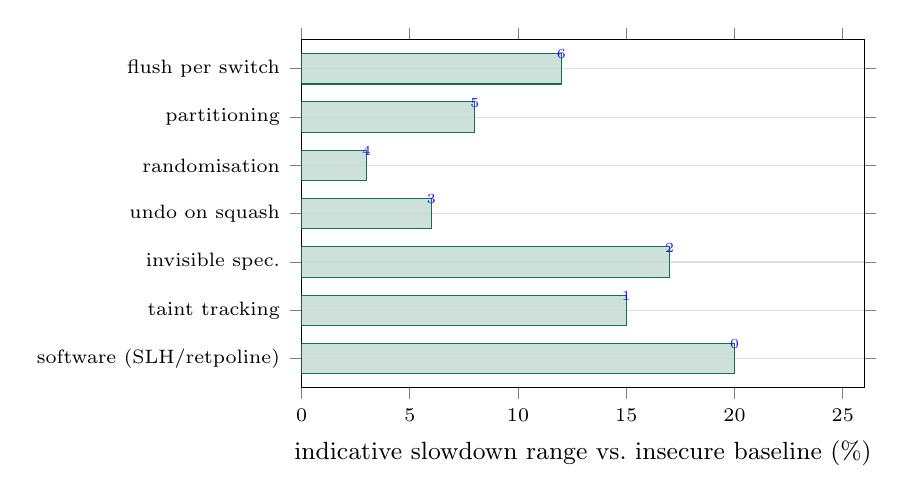
\begin{tikzpicture}
\begin{axis}[
  barstyle, height=6.0cm, width=0.72\linewidth,
  xbar, bar width=11pt, xmin=0, xmax=26,
  symbolic y coords={{software (SLH/retpoline)}, {taint tracking}, {invisible spec.},
                     {undo on squash}, {randomisation}, {partitioning}, {flush per switch}},
  ytick=data, yticklabel style={font=\scriptsize},
  xlabel={indicative slowdown range vs.\ insecure baseline (\%)},
  nodes near coords, nodes near coords style={font=\tiny},
  ]
  \addplot+[fill=defense!25, draw=defense] coordinates {
    (20,{software (SLH/retpoline)}) (15,{taint tracking}) (17,{invisible spec.})
    (6,{undo on squash}) (3,{randomisation}) (8,{partitioning}) (12,{flush per switch})};
\end{axis}
\end{tikzpicture}
\caption[Indicative cost by defence class]{Indicative slowdown by defence class.
\textbf{These are order-of-magnitude illustrations synthesised from the
qualitative descriptions in \Cref{tab:defenses}, not measurements, and not
directly attributable to any single paper}, for the reasons given in
\Cref{sec:incomparable}. Their purpose is to show that the classes differ by
roughly an order of magnitude in cost, and that the cheapest defences are the
ones with the narrowest guarantees. Measured replacements are experiment~E5 of
\Cref{ch:evalplan}.}
\label{fig:overheads}
\end{figure}

Two patterns in \Cref{fig:overheads} hold across the literature, and this paper
reports them as findings of the survey.

\textbf{Cost tracks breadth of guarantee.} Randomisation is cheap because it
defends one specific attack step (eviction-set construction) and leaves
shared-memory channels intact. Taint tracking is expensive because it defends a
class of information flows regardless of structure. This is not a defect of the
expensive schemes; it is the price of a stronger claim.

\textbf{Cost distribution matters more than the mean.} Partitioning and flushing
have low mean costs and long tails: workloads at a capacity cliff or with a high
context-switch rate pay far more than the average. Reporting only the mean
conceals the cases a system designer most needs to plan for.

\section{Energy and area}

Performance is only one axis. From \Cref{eq:power}, a defence that increases
memory traffic raises activity in the most energy-expensive part of the system.
Flushing defences are the clearest case: they may cost few cycles on a
compute-bound workload yet still force DRAM refills whose energy cost is
disproportionate. Conversely, defences that \emph{delay} execution without adding
traffic (delay-on-miss, taint-based blocking) mostly lengthen $T$ while leaving
$E$ per instruction roughly unchanged, so their EDP penalty
(\Cref{eq:edp}) is milder than their slowdown suggests.

\Cref{tab:area} summarises the storage and logic that each class adds. Area is
the axis on which embedded RISC-V cores are most sensitive: a defence costing a
few kilobytes of shadow storage is negligible on an application-class core and
prohibitive on a microcontroller-class one.

\begin{table}[t]
\centering
\caption[Storage and logic overheads by defence class]{Storage and logic added by
each defence class, and the core class for which it is a plausible choice.
Qualitative in v0.1; the synthesis results that populate this table numerically
are experiment~E6 of \Cref{ch:evalplan}.}
\label{tab:area}
\footnotesize
\begin{tabularx}{\linewidth}{@{}>{\raggedright\arraybackslash}p{3.0cm}>{\raggedright\arraybackslash}p{4.3cm}X@{}}
\toprule
\textbf{Class} & \textbf{Added hardware} & \textbf{Plausible target} \\
\midrule
Way partitioning & Per-way domain bits; allocation-policy logic in the cache controller &
Application and server class; needs a domain-ID notion in the privileged architecture. \\
Page colouring & None (software only) & Any class, including embedded; costs OS complexity. \\
Temporal flush & Flush sequencer; timing-normalisation counter &
Embedded and real-time cores, where the switch rate is bounded and the state is small. \\
Randomisation & Low-latency block cipher or keyed hash in the index path; re-keying state machine &
Server-class LLCs, where the latency addition is amortised. \\
Invisible speculation & Speculative buffers sized to the load queue; validation logic at commit &
Out-of-order cores only; meaningless on an in-order core. \\
Undo on squash & Rollback logs and restoration paths in the cache &
Out-of-order cores; interacts with coherence. \\
Taint tracking & Taint bits per physical register and queue entry; propagation logic &
Out-of-order cores; area modest, verification effort large. \\
Enclaves (PMP-based) & PMP/ePMP registers, flush-on-entry logic, monitor firmware &
All classes; already partly present in RISC-V. \\
\bottomrule
\end{tabularx}
\end{table}

\section{The design space, not a winner}

\Cref{fig:pareto} plots the two axes against each other, with the qualitative
strength of the guarantee on one axis and cost on the other. The point of the
figure is that there is no dominant mechanism: the frontier is populated, and the
right choice depends on the core class and the deployment.

\begin{figure}[t]
\centering
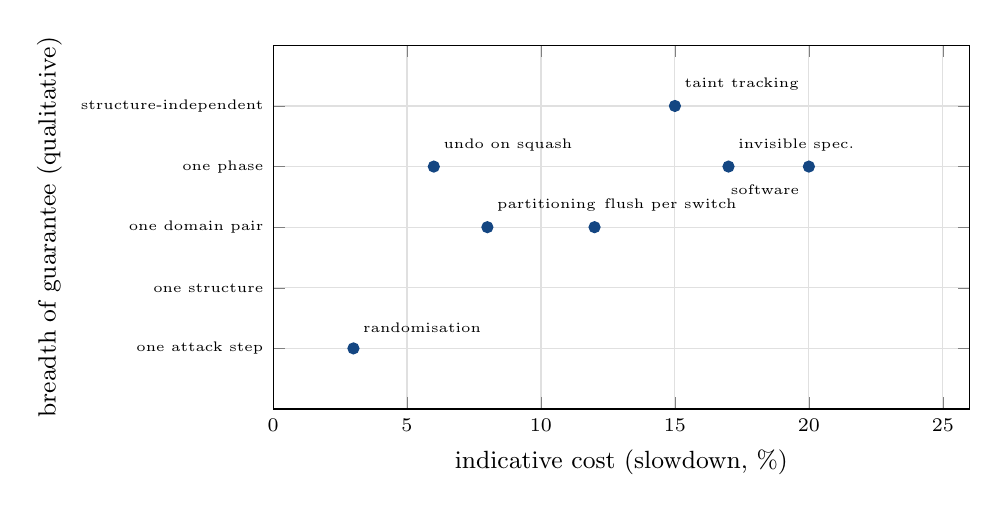
\begin{tikzpicture}
\begin{axis}[
  height=6.2cm, width=0.86\linewidth,
  xlabel={indicative cost (slowdown, \%)},
  ylabel={breadth of guarantee (qualitative)},
  xmin=0, xmax=26, ymin=0, ymax=6,
  ytick={1,2,3,4,5},
  yticklabels={one attack step, one structure, one domain pair, one phase, structure-independent},
  yticklabel style={font=\tiny}, xticklabel style={font=\scriptsize},
  label style={font=\small},
  ymajorgrids, xmajorgrids, grid style={draw=black!12},
  ]
  \addplot[only marks, mark=*, mark size=2pt, draw=accent, fill=accent]
    coordinates {(3,1) (8,3) (12,3) (6,4) (17,4) (15,5) (20,4)};
  \node[font=\tiny, anchor=south west] at (axis cs:3,1.1)  {randomisation};
  \node[font=\tiny, anchor=south west] at (axis cs:8,3.1)  {partitioning};
  \node[font=\tiny, anchor=south west] at (axis cs:12,3.1) {flush per switch};
  \node[font=\tiny, anchor=south west] at (axis cs:6,4.1)  {undo on squash};
  \node[font=\tiny, anchor=south west] at (axis cs:17,4.1) {invisible spec.};
  \node[font=\tiny, anchor=south west] at (axis cs:15,5.1) {taint tracking};
  \node[font=\tiny, anchor=north east] at (axis cs:20,3.86) {software};
\end{axis}
\end{tikzpicture}
\caption[Cost versus breadth of guarantee]{The design space. Both axes are
indicative: the horizontal from \Cref{fig:overheads}, the vertical from the
coverage analysis of \Cref{tab:defenses}. \textbf{Not measured data.} The figure
supports one claim only, and a firm one: no mechanism dominates, so a real
system composes several, and composition is what \Cref{ch:evalplan} sets out to
measure.}
\label{fig:pareto}
\end{figure}

\begin{draftnote}
For v0.2 and v0.3, \Cref{fig:overheads,fig:pareto} and \Cref{tab:area} will be
rebuilt from measured data on a single RISC-V platform, so that every point has
the same baseline, the same benchmarks and the same reporting convention. Until
then all three are explicitly labelled as illustrative, and every number in
\Cref{tab:defenses} is attributed to its source. This labelling discipline is a
deliberate choice: the alternative (an authoritative-looking chart mixing
incomparable numbers) is the most common failure mode of surveys in this area.
\end{draftnote}

\chapter{Evaluation Plan for v0.2 and v0.3}
\label{ch:evalplan}

\section{Purpose and honesty about status}

This chapter specifies the experimental work that will turn the illustrative
figures of \Cref{ch:tradeoffs} into measurements. Nothing in it has been run yet;
it is a plan, and it is stated in enough detail to be criticised now rather than
after the effort has been spent.

The guiding requirement follows from \Cref{sec:incomparable}: to compare
defences meaningfully, all measurements must share one baseline core, one
benchmark set, one reporting convention, and one definition of the threat
covered. The plan is therefore organised as a single platform plus a sequence of
experiments on it.

\section{Platform}

\Cref{tab:platform} fixes the intended platform. The choice of an open RISC-V
core is not incidental, it is what makes the chain from RTL structure to
measured leak to measured defence cost closable at all
(\Cref{sec:whyriscv}).

\begin{table}[t]
\centering
\caption[Intended evaluation platform]{Intended evaluation platform. Two
configurations are used throughout so that the in-order/out-of-order distinction
of \Cref{ch:transient} can be measured rather than asserted.}
\label{tab:platform}
\footnotesize
\begin{tabularx}{\linewidth}{@{}p{3.1cm}X@{}}
\toprule
\textbf{Component} & \textbf{Choice and rationale} \\
\midrule
Cores & Rocket (in-order, 5-stage)~\citep{asanovic2016rocket} and BOOM/SonicBOOM
(superscalar out-of-order)~\citep{zhao2020sonicboom}. The pair isolates the
effect of the speculation window. \\
Integration & Chipyard~\citep{amid2020chipyard}, which packages both cores with a
configurable memory hierarchy and a consistent build flow. \\
Execution & Cycle-accurate RTL simulation for microbenchmarks; FPGA-accelerated
simulation~\citep{karandikar2018firesim} for anything needing a booted Linux and
long runs. \\
Cross-check & gem5~\citep{binkert2011gem5,lowepower2020gem5} in RISC-V mode, used
only to sanity-check trends, never as a primary source, since simulator cache
timing is exactly the quantity under study. \\
Workloads & A microbenchmark set written for this paper (pointer chase, eviction
set construction, Spectre-v1 gadget) plus an embedded suite for whole-program
IPC. Selection to be finalised in v0.2. \\
Metrics & IPC and slowdown (\Cref{eq:iron,eq:slowdown}); AMAT
(\Cref{eq:amat}); energy and EDP (\Cref{eq:power,eq:edp}); post-synthesis area
where a defence is implemented in RTL. \\
\bottomrule
\end{tabularx}
\end{table}

\section{Experiments}

\Cref{tab:experiments} lists the seven planned experiments. Each is tied to one
of the research questions of \Cref{sec:rqs} and to the specific figure or table
in this draft that it is intended to replace, so that no experiment is run
without a place for its result to land.

\begin{table}[t]
\centering
\caption[Planned experiments]{Planned experiments, each tied to the research
question it answers (\Cref{sec:rqs}) and to the figure or table it replaces.}
\label{tab:experiments}
\footnotesize
\begin{tabularx}{\linewidth}{@{}p{0.8cm}p{3.8cm}p{1.4cm}X@{}}
\toprule
\textbf{ID} & \textbf{Experiment} & \textbf{Answers} & \textbf{Deliverable} \\
\midrule
E1 & Latency characterisation: measured hit/miss distributions for L1, L2, LLC and
DRAM on both cores & RQ1, RQ2 & Measured replacements for
\Cref{fig:hierarchy,fig:histogram} \\
E2 & Eviction-set construction on the configured LLC, with time-to-construct as a
function of associativity and page size & RQ2 &
Bandwidth figures for \Cref{tab:primitives} \\
E3 & Speculation-window characterisation: transient instructions executed as a
function of ROB size on BOOM & RQ3 & New figure for \Cref{ch:transient} \\
E4 & Spectre-v1 replication on BOOM using \Cref{lst:spectre1rv}, with recovered
bits per second and error rate & RQ3 & Evidence row in \Cref{tab:variants} \\
E5 & Cost of one defence per class, implemented or configured on the same
platform, over the same workloads & RQ5 & Measured
\Cref{fig:overheads,fig:pareto} \\
E6 & Post-synthesis area and frequency impact for the RTL-implemented defence &
RQ5 & Numeric \Cref{tab:area} \\
E7 & Composition: two defences from different taxonomy branches applied together,
testing whether costs add and whether coverage composes & RQ4, RQ5 &
New section in \Cref{ch:defenses} \\
\bottomrule
\end{tabularx}
\end{table}

E7 is the experiment with the highest intellectual return and the highest risk.
The literature evaluates defences singly; a real system will deploy several, and
whether their costs add linearly is unknown. If time forces a reduction in scope,
E7 is the one to attempt last and the one whose partial result is still
publishable within the paper.

\section{Threats to validity}

Three, stated in advance so that the results can be read properly. First,
simulated timing is not silicon timing, so results establish trends and relative
costs rather than absolute cycle counts. Second, a microbenchmark set written by the
author to exercise a channel will flatter attacks relative to real workloads; the
whole-program measurements exist to counterbalance this. Third, implementing a
defence oneself risks an implementation that is less optimised than its authors'
version, which would overstate its cost; where a defence is reimplemented rather
than configured, the reported number will be labelled as such.

\section{Schedule}

\Cref{fig:gantt} maps the experiments onto the four submission points.

\begin{figure}[!ht]
\centering
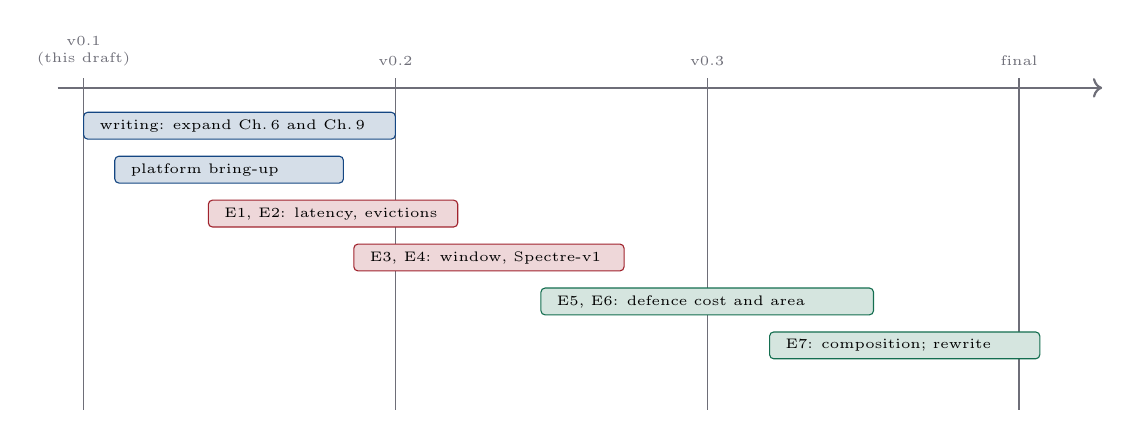
\begin{tikzpicture}[x=1.32cm, y=0.62cm, every node/.style={font=\scriptsize}]
  % axis: milestone rules on the background layer so the bars always sit on top
  \begin{scope}[on background layer]
    \foreach \i in {0,3,6,9} {\draw[muted] (\i,0.6) -- (\i,-6.2);}
  \end{scope}
  \foreach \i/\lab in {0/{v0.1\\(this draft)}, 3/{v0.2}, 6/{v0.3}, 9/{final}}
     {\node[align=center, anchor=south, font=\tiny, text=muted] at (\i,0.65) {\lab};}
  \draw[->, muted, thick] (-0.25,0.4) -- (9.8,0.4);
  % bars
  \foreach \r/\start/\len/\lab/\col in {%
      1/0/3/{writing: expand Ch.\,6 and Ch.\,9}/accent,
      2/0.3/2.2/{platform bring-up}/accent,
      3/1.2/2.4/{E1, E2: latency, evictions}/attack,
      4/2.6/2.6/{E3, E4: window, Spectre-v1}/attack,
      5/4.4/3.2/{E5, E6: defence cost and area}/defense,
      6/6.6/2.6/{E7: composition; rewrite}/defense}
  {
    \draw[fill=\col!18, draw=\col, rounded corners=1.5pt]
         (\start,-\r*0.9+0.25) rectangle ++(\len,0.55);
    \node[anchor=west, font=\tiny] at (\start+0.06,-\r*0.9+0.52) {\lab};
  }
\end{tikzpicture}
\caption[Schedule to the final version]{Schedule from this draft to the final
submission. Writing and experimentation overlap deliberately: the chapters with
the largest identified gaps (\Cref{ch:memsys} and \Cref{ch:defenses}) are
expanded first, so that the experimental results have somewhere to land.}
\label{fig:gantt}
\end{figure}

Two dependencies are worth naming explicitly, because they determine what gets
cut if the schedule slips. Platform bring-up gates everything downstream: if
Chipyard is not building and booting both core configurations by the v0.2
deadline, experiments E1--E4 slip, and the correct response is to narrow the
platform to a single core rather than to report numbers that have not been
verified. Second, E5 assumes that at least one defence per class is either
configurable in existing RTL or implementable within the time budget. Where it is
not, the fallback is to measure a partitioning scheme (which needs no new RTL,
only allocation-policy changes) and to continue reporting the remaining
classes from the literature, labelled as such, exactly as this draft does.

\chapter{Conclusion}
\label{ch:conclusion}

\section{What the paper has argued so far}

The argument of this draft can be compressed into four claims, each established
in a specific chapter and each following from the prescribed textbook's own
account of how processors are built.

\textbf{First, the leak is structural, not accidental.} An ISA constrains values
and says nothing about time (\Cref{eq:contract}). Every mechanism that makes a
processor fast (caching, translation caching, prediction, speculation, sharing) works by remembering something about what ran before, and remembered state is
observable through timing. \Cref{ch:memories} located that observability in the
physics of the array; \Cref{ch:proc} showed that a machine without those
mechanisms has almost no channels and is unusably slow.

\textbf{Second, speculation converts a side channel into a read primitive.}
Precise exceptions restore architectural state exactly and \uarchadj{} state not at
all (\Cref{sec:precise}). Spectre works on that asymmetry alone, and it cannot be
patched at the ISA level because the mechanism being exploited is the mechanism
providing the performance.

\textbf{Third, RISC-V is neither immune nor merely a victim.} The attacks
transfer, and have been demonstrated on open out-of-order RISC-V
cores~\citep{gonzalez2019replicating}. But the open specification makes it
possible to say which vulnerabilities are architectural and which are
implementation choices: Meltdown-type forwarding and speculative store
disambiguation are both choices, not requirements, as \Cref{tab:variants} sets
out. The open RTL then makes it possible to measure the cost of changing them.

\textbf{Fourth, price matters more than possibility.} Every channel in this
paper can be closed; \Cref{fig:datapath} is the limiting case. What a designer
actually has to decide is which defence closes which phase of
\Cref{fig:anatomy}, what it leaves open, and what it costs in IPC, energy and
area. The honest answer today is that the published numbers are not comparable
(\Cref{sec:incomparable}), so this paper ends with a plan to produce numbers
that are.

\section{What this draft does not yet establish}

Three limitations, stated plainly. No measurement in this paper is the author's
own; every quantitative claim is attributed and every illustrative figure is
labelled as such. The leakage model of \Cref{sec:leakmodel} is informal. And the
composition question (whether defences from different taxonomy branches add
their costs or interact) is posed but not answered, and is the most
substantive open question the paper identifies.

\section{Roadmap}

Versions v0.2 and v0.3 will execute the plan of \Cref{ch:evalplan}, expand
\Cref{ch:memsys} and \Cref{ch:defenses} (the two chapters with the largest
identified gaps), formalise the leakage model, and replace every illustrative
figure with a measured one. \Cref{app:changelog} gives the item-by-item plan and
the word budget for reaching the target length.

%%=====================================================================
\appendix
%% cleveref names chapter-level labels "Chapter" unless told otherwise. Without
%% this alias, every \Cref to an appendix prints "Chapter A" under pdfLaTeX
%% (Tectonic happens to get it right, which is exactly why it is easy to miss).
\crefalias{chapter}{appendix}
%%=====================================================================

\chapter{Plagiarism Report}
\label{app:plagiarism}
\section{Declaration of originality}

The text, structure, figures and analysis of this paper are my own work, prepared
for \coursecode{}: \coursetitle{} and submitted for no other course. This
appendix states what has been checked in this draft and, equally, what has not.

\section{Citation practice}

\begin{itemize}
  \item \textbf{Every quantitative figure belongs to whoever measured it.} The
        slowdowns, area and energy costs collated in \Cref{ch:defenses,ch:tradeoffs}
        are as reported by the original authors, on their own platforms and
        benchmark suites, and are attributed in the text as well as in the table
        cell. This draft contains no measurement of my own.
  \item \textbf{Illustrative figures say so.} Where a plot shows the shape of an
        effect rather than data, its caption and the body text label it
        illustrative. There are four such figures and no others:
        \Cref{fig:hierarchy}, \Cref{fig:histogram}, \Cref{fig:overheads} and
        \Cref{fig:pareto}.
  \item \textbf{All 62 sources are cited.} Every record in the project's Zotero
        library is cited at least once in the body, and every citation resolves to
        a record whose authors, venue, year, pages and DOI were checked against the
        publisher's own metadata (\Cref{app:toolchain}).
\end{itemize}

\section{Similarity checking performed}

\begin{table}[ht]
\centering
\caption{Checks carried out on draft \draftversion{}. No similarity percentage
appears anywhere in this document, because none has been generated.}
\label{tab:plagchecks}
\footnotesize
\begin{tabularx}{\linewidth}{@{}p{4.4cm}p{1.9cm}X@{}}
\toprule
\textbf{Check} & \textbf{Status} & \textbf{Notes} \\
\midrule
Institutional similarity tool (Turnitin, Ouriginal or equivalent) & \textbf{Not run} &
I have no access to the institute's tool for a draft submission. No percentage is
claimed, estimated or implied here. \\
\addlinespace
Source-by-source manual check & Done & One Zotero note per cited work records what
was taken from it and whether it was quoted or paraphrased. \\
\addlinespace
Verbatim-material audit & Done & Reproduced text is confined to the categories of
\Cref{sec:plagexpected}, each attributed. \\
\addlinespace
Bibliographic metadata verification & Done & Checked venue by venue against DBLP
and Crossref. \\
\addlinespace
Figure provenance & Done & Every figure is generated from TikZ or
\texttt{pgfplots} source in this file; none is copied or traced. \\
\addlinespace
Reuse of my own earlier work & None & No part of this paper has been submitted
elsewhere. \\
\bottomrule
\end{tabularx}
\end{table}

\section{Material a similarity checker would legitimately flag}
\label{sec:plagexpected}

When the tool is run, four categories of overlap should be expected and are not
misconduct:

\begin{enumerate}
  \item \textbf{Textbook section titles.} The mapping tables of \Cref{app:tocmap}
        quote the section headings of the prescribed textbook
        \citep{sarangi2025basic} verbatim, so that a reader can align this paper
        against the syllabus heading by heading.
  \item \textbf{Standard technical terminology.} Phrases such as ``bounds-check
        bypass'' and ``inclusive last-level cache'' are the field's fixed
        vocabulary; substituting synonyms would obscure rather than clarify.
  \item \textbf{The canonical Spectre-v1 gadget.} \Cref{lst:spectre1} is quoted
        from Kocher \etal{} \citep{kocher2019spectre} and cited as theirs in the
        caption and the text. The literature reasons about that exact fragment, so
        rewriting it would defeat the comparison.
  \item \textbf{Bibliography entries}, which are by construction identical to the
        publishers' own records.
\end{enumerate}

\begin{draftnote}
For v0.2: run the institute's similarity-checking tool once access is granted for
coursework, then replace the first row of \Cref{tab:plagchecks} with the tool
name, the date of the run and the reported percentage, together with the
per-category breakdown of matched text. Any match falling outside the four
categories above will be quoted here and corrected in the body.
\end{draftnote}

\chapter{Reading Indices}
\label{app:readability}
The course guideline asks for reading indices. This appendix reports eight
standard readability measures for the running prose of this report, states
exactly what text they were computed over, and reads the result honestly.

\section{What was measured, and how}

The indices are computed over the \textbf{body prose of \Cref{ch:intro} to
\Cref{ch:conclusion}} only. The front matter, the appendices, the bibliography,
every table, every figure and caption, every code listing, every displayed
equation and every \LaTeX{} command were removed before counting, so that the
numbers describe sentences a reader actually reads rather than the surrounding
apparatus. Inline mathematics and code identifiers were each replaced by a
single token so that they count as one word and do not distort syllable counts.
Sentence boundaries were taken at \texttt{.}, \texttt{!} and \texttt{?} followed
by a capital, with the usual abbreviations (\eg{} \texttt{e.g.},
\texttt{i.e.}, \texttt{et al.}) protected. Syllables were counted by the standard
vowel-group heuristic with silent-\texttt{e} correction.

The measurement is therefore reproducible from the submitted source, and the
counts it rests on are given in \Cref{tab:readcounts}.

\begin{table}[ht]
\centering
\caption{Counts underlying the indices, over the body prose of
\Cref{ch:intro}--\Cref{ch:conclusion}.}
\label{tab:readcounts}
\footnotesize
\begin{tabularx}{\linewidth}{@{}Xr@{}}
\toprule
\textbf{Quantity} & \textbf{Value} \\
\midrule
Sentences & 426 \\
Words & 11,014 \\
Syllables & 18,860 \\
Polysyllabic words (3 or more syllables) & 2,152 \\
Long words (7 or more letters) & 3,434 \\
Letters & 57,727 \\
\addlinespace
Average sentence length (words) & 25.85 \\
Average word length (syllables) & 1.712 \\
\bottomrule
\end{tabularx}
\end{table}

\section{The indices}

\Cref{tab:readindices} gives the eight indices. They fall into two families that
have to be read differently. Six of them (Flesch--Kincaid, Gunning Fog, SMOG,
Coleman--Liau, the Automated Readability Index and, loosely, RIX) return a
\emph{grade level}: the number of years of formal education a reader is assumed
to have, so a higher number means a harder text. The other two invert that
scale. Flesch Reading Ease runs from 0 to 100 with \emph{higher} meaning easier,
and LIX is a difficulty score on its own scale where higher again means harder.
A document can therefore look inconsistent at a glance while being perfectly
consistent underneath, which is why both the value and its interpretation are
given in every row.

The measures also disagree by construction about what makes text hard. Flesch
and SMOG count syllables, Coleman--Liau and the Automated Readability Index
count letters and characters instead, and LIX and RIX count long words. A
technical vocabulary of long but familiar words pushes the letter-based and
long-word measures up faster than the syllable-based ones, so the spread between
them is itself informative rather than a sign that one of them is wrong.

\begin{table}[htbp]
\centering
\caption{Reading indices for the body prose. Interpretations are the
conventional ones used by \texttt{analyzemywriting.com}.}
\label{tab:readindices}
\footnotesize
\begin{tabularx}{\linewidth}{@{}p{5.4cm}rX@{}}
\toprule
\textbf{Index} & \textbf{Value} & \textbf{Interpretation} \\
\midrule
Flesch Reading Ease & 35.7 & 0--100, higher is easier. Difficult, college level. \\
Flesch--Kincaid Grade Level & 14.7 & US school grade needed. \\
Gunning Fog Index & 18.2 & Years of formal education needed. \\
SMOG Index & 16.0 & Grade level, tuned for dense material. \\
Coleman--Liau Index & 13.9 & Grade level, from letters not syllables. \\
Automated Readability Index & 16.2 & Grade level, from characters per word. \\
LIX (L\"asbarhetsindex) & 57.0 & Very difficult; technical and academic. \\
RIX & 8.06 & Long words per sentence. \\
\bottomrule
\end{tabularx}
\end{table}

\section{Reading the result}

The indices agree with each other and with what the document is. Six of the
eight grade-level measures land between 13 and 19, that is, undergraduate to
postgraduate; the Flesch Reading Ease of 35.7 and the LIX of 57.0 put the text in
the same band. That is the expected register for a technical paper whose subject
is processor microarchitecture, and it is the register of the literature it
surveys.

Two properties of the subject matter push the indices upward and cannot be
removed without damaging the paper. The first is vocabulary: words like
\emph{microarchitectural}, \emph{associativity} and \emph{speculation} are
polysyllabic and are the correct terms, and 2,152 of the 11,014 words counted are
polysyllabic. Replacing them with shorter words would make the paper less
precise, not more readable, which is why the Glossary exists instead. The second
is sentence length: the average sentence runs 25.85 words because the argument is
frequently conditional, of the form \emph{this structure leaks under these
conditions and not under those}, and splitting such sentences tends to separate a
claim from the qualification that makes it true.

Where the indices are actionable, they have been acted on. The prose was revised
to remove the constructions that inflate sentence length without adding meaning,
and \Cref{app:changelog} records that pass. What remains is length that carries
content.

\begin{draftnote}
For v0.2: recompute these indices after the chapters expand towards the target
length, and report them per chapter as well as in aggregate, so that any chapter
drifting well above the others is caught and revised.
\end{draftnote}

\chapter{Cost Metrics: Definitions and Validity Conditions}
\label{app:metrics}

This appendix collects the performance, power and energy definitions used to
price defences in \Cref{ch:tradeoffs}. It is separated from \Cref{sec:metrics}
because it is an explanation rather than part of the argument, and it runs to
more than half a page.

Textbook \SecRef{10.9.3} and \SecRef{10.10} supply the vocabulary used for the
whole of \Cref{ch:tradeoffs}. Execution time is
\begin{equation}
  T \;=\; \frac{N_{\text{inst}} \times \text{CPI}}{f}
  \;=\; \frac{N_{\text{inst}}}{\text{IPC} \times f},
  \label{eq:iron}
\end{equation}
with $N_{\text{inst}}$ the dynamic instruction count, CPI the cycles per
instruction, IPC $=1/\text{CPI}$, and $f$ the clock frequency. A defence can
degrade any of the three factors, and \emph{which} factor it degrades matters:

\begin{itemize}
  \item Defences that add instructions (speculative load hardening, retpolines,
        explicit fences) increase $N_{\text{inst}}$.
  \item Defences that delay execution (delay-on-miss, invisible speculation,
        taint-based blocking) increase CPI while leaving $N_{\text{inst}}$ alone.
  \item Defences that add logic to a critical path (extra tag comparisons,
        address encryption) can reduce $f$. This is rarely reported, and is a systematic
        gap in the literature that \Cref{ch:evalplan} proposes to address.
\end{itemize}

Relative slowdown against an insecure baseline is reported throughout as
\begin{equation}
  S \;=\; \frac{T_{\text{defended}}}{T_{\text{baseline}}} - 1 ,
  \label{eq:slowdown}
\end{equation}
which reduces to the ratio of IPCs,
$S = \text{IPC}_{\text{baseline}}/\text{IPC}_{\text{defended}} - 1$, only when the
defence leaves both $N_{\text{inst}}$ and $f$ unchanged. That condition fails
precisely for the first and third bullets above, so a slowdown quoted as an IPC
ratio for a defence that inserts instructions, or that costs frequency, is not
the same quantity as one quoted as a time ratio. \Cref{ch:evalplan} reports
execution time and states $N_{\text{inst}}$ and $f$ alongside it for this
reason.

For energy, dynamic power in a CMOS core follows
\begin{equation}
  P_{\text{dyn}} \;=\; \alpha\,C\,V_{dd}^{2}\,f ,
  \label{eq:power}
\end{equation}
where $\alpha$ is the activity factor (\SecRef{10.10.2}).\footnote{The textbook
develops the closely related $ED^{2}$ metric in \SecRef{10.10.5}; this paper uses
the energy-delay product, and states which is meant wherever a single figure of
merit is quoted.} This equation is the
reason cache-flushing defences are not free even when they cost no cycles:
refilling a flushed cache raises $\alpha$ in the memory hierarchy and drives
additional DRAM traffic, which is expensive per access. Because performance and
power trade against each other, the honest single-number comparison is the\index{energy-delay product (EDP)}
energy-delay product,
\begin{equation}
  \text{EDP} \;=\; E \times T \;=\; P_{\text{avg}} \times T^{2}.
  \label{eq:edp}
\end{equation}

\begin{draftnote}
For v0.2: \Cref{eq:iron,eq:slowdown,eq:power,eq:edp} will be instantiated with
measured numbers from the author's own runs (\Cref{ch:evalplan}), and this
section will gain a worked example computing the EDP cost of flushing a
\SI{32}{\kibi\byte} L1 at every context switch on CVA6, cross-checked against the
figures reported by Wistoff \etal~\citep{wistoff2021fencet}. Also to be added: a
short treatment of Amdahl's law applied to defences that only slow down a subset
of instructions (\eg{} loads only). Target: +2 pages.
\end{draftnote}

\chapter{Detailed Mapping to the Textbook Table of Contents}
\label{app:tocmap}

\Cref{tab:tocmap} in \Cref{sec:tocmap} gives the mapping at chapter and section
granularity. \Cref{tab:tocdetail} below expands it to sub-section granularity, as
the assignment requires, stating for each sub-section the specific role it plays.
The textbook is S.~R.~Sarangi, \textit{Basic Computer Architecture},
\textbf{Version 3.09, 8 October 2025}~\citep{sarangi2025basic}, available at
\url{https://srsarangi.github.io/archbook/archbook.pdf}. Every section number
below was checked against that edition's Table of Contents; because the book is
revised periodically, the version is stated so that the mapping can be re-checked
against any later revision.

No second textbook is used as a structural guideline. Hennessy and
Patterson~\citep{hennessy2019quantitative} is cited as a secondary source only,
and every other cited work is a research paper or specification used as evidence
rather than as skeleton. Two topics in this paper have \emph{no} counterpart in
the prescribed text and are drawn entirely from the research literature: cache
partitioning and colouring viewed as defences (\Cref{sec:partitioning}), and the
whole of transient-execution attacks and their defences
(\Cref{ch:transient,ch:defenses}).

\footnotesize
\begin{longtable}{@{}p{2.0cm}p{3.4cm}p{8.1cm}@{}}
\caption{Sub-section-level mapping between the prescribed textbook and this term
paper.\label{tab:tocdetail}}\\
\toprule
\textbf{Sub-section} & \textbf{Topic} & \textbf{Role in this paper} \\
\midrule
\endfirsthead
\multicolumn{3}{@{}l}{\footnotesize\itshape \Cref{tab:tocdetail} continued from previous page}\\
\toprule
\textbf{Sub-section} & \textbf{Topic} & \textbf{Role in this paper} \\
\midrule
\endhead
\midrule
\multicolumn{3}{r@{}}{\footnotesize\itshape continued on next page}\\
\endfoot
\bottomrule
\endlastfoot

\multicolumn{3}{@{}l}{\textbf{Chapter 1, Introduction to Computer Architecture (supporting)}}\\
Ch.~1 opening & Definitions of \emph{architecture} and \emph{organization} &
Source of the central distinction of \Cref{sec:contract}: architecture is the
view presented to software designers, organization is the hardware
implementation. The ISA constrains results, not timing. \\
\S1.4 & The Language of Instructions & Establishes the ISA as the language shared
by hardware and software, used in \Cref{ch:isa} to argue that openness of the
contract does not imply absence of implementation leakage. \\
\S1.5 & Instruction Set Design & The completeness, conciseness, genericity and
simplicity criteria; \Cref{ch:isa} observes that \emph{constant-time behaviour}
is not among them. \\
\S1.7 & Design of Practical Machines & Harvard and Von Neumann organisations, and
the move to registers. Supplies the theme that implementation pressure shapes the
specification, illustrated by the fixed register-field positions of
\Cref{fig:encoding}. \\
\addlinespace
\multicolumn{3}{@{}l}{\textbf{Chapter 6, RISC-V Assembly Language (primary)}}\\
\S6.1.1 & RISC-V Base ISAs and Extensions & \Cref{tab:extensions}: which
extensions make timing promises and which do not. \\
\S6.1.2 & View of Registers & \Cref{ch:isa}: architectural registers are scrubbed
on a context switch; predictors are not. \\
\S6.3.1 & Conditional Branches & The instructions that train the direction
predictor (\Cref{fig:predictors}); the mistrained branch of Spectre-v1. \\
\S6.3.2 & Unconditional Branches & \code{jal}/\code{jalr}: the BTB and
return-address-stack channels, and Spectre-v2 and Retbleed. \\
\S6.3.3 & Load and Store Instructions & The data-dependent effective address:
the transmitter of \Cref{lst:leak}. \\
\S6.5 & Instruction Encoding & \Cref{fig:encoding}; also the argument that
security instructions must compete for finite encoding space. \\
\addlinespace
\multicolumn{3}{@{}l}{\textbf{Chapter 7, Logic Gates, Registers and Memories (supporting)}}\\
\S7.4.1 & Static RAM (SRAM) & \Cref{fig:sram,fig:array,fig:readtiming}: the cell,
the array around it, and the read timing that attacks measure. \\
\S7.4.2 & Content Addressable Memory (CAM) & \Cref{ch:memories}: TLBs, MSHRs and
store queues use associative lookup, so match/no-match is a timing path. \\
\S7.4.3 & Dynamic RAM (DRAM) & The row buffer as the coarsest member of the
channel family (\Cref{tab:statepartition}). \\
\addlinespace
\multicolumn{3}{@{}l}{\textbf{Chapter 9, Processor Design (primary)}}\\
\S9.1 & Design of a Basic Processor & Frames the reference machine of
\Cref{ch:proc}. \\
\S9.2.1 & Instruction Fetch: Fetch Unit & Where the I-cache and the predictors
are later inserted. \\
\S9.2.2 & Data Path and Control Path & The separation that \Cref{fig:datapath}
draws, and that \Cref{ch:pipeline} gives memory to. \\
\S9.2.3 & Operand Fetch Unit & Register read in parallel with decode; the
baseline for rename and issue queues. \\
\S9.2.4 & Execute Unit & The baseline for multiple functional units and the
port-contention channel. \\
\S9.2.5 & Memory Access Unit & The stage that \Cref{ch:memsys} is entirely
about. \\
\S9.2.6 & Register Writeback Unit & Completes the architectural contract;
contrasted with commit in an out-of-order core. \\
\S9.2.7 & The Data Path & The assembled reference machine of
\Cref{fig:datapath}. \\
\S9.3 & The Control Unit & Used to make the point that a branch predictor is a
control unit with memory. \\
\addlinespace
\multicolumn{3}{@{}l}{\textbf{Chapter 10, Principles of Pipelining (primary)}}\\
\S10.1--\S10.3 & A pipelined processor, design of a simple pipeline, pipeline
stages & \Cref{fig:pipeline}: several instructions in flight; the origin of
control hazards. \\
\S10.4 & Pipeline Hazards (data, control, structural) & \Cref{tab:hazards}: each
hazard resolution leaves a security-relevant residue. \\
\S10.8, \S10.8.2 & Support for interrupts/exceptions; exceptions & The mechanism
whose semantics \Cref{sec:precise} examines. \\
\S10.8.3 & Precise Exceptions & The single most important background result in
the paper: architectural restoration is complete, \uarchadj{} restoration is not. \\
\S10.9.3 & Performance of a Non-Ideal Pipeline & \Cref{eq:iron,eq:slowdown}: how
defence cost is measured. \\
\S10.10.2, \S10.10.5 & Dynamic power; the $ED^{2}$ metric &
\Cref{eq:power,eq:edp}: energy and energy-delay cost of flushing and refilling. \\
\S10.11.1 & Branch Prediction & \Cref{fig:predictors}: the shared, index-aliased,
never-scrubbed structures behind Spectre-v2. \\
\S10.11.4 & Out-of-Order Pipelines & \Cref{fig:ooo}: the execution window whose
size bounds transient-attack capability. \\
\addlinespace
\multicolumn{3}{@{}l}{\textbf{Chapter 11, The Memory System (primary)}}\\
\S11.1.2--\S11.1.5 & Memory access patterns; temporal and spatial locality &
Why the latency gap of \Cref{fig:hierarchy} exists and cannot be designed away. \\
\S11.1.6--\S11.1.8 & Utilising locality; hierarchical memory; cache blocks &
Block granularity = channel granularity (\Cref{fig:addrsplit}). \\
\S11.2 & Caches: lookup and design, read/write, insert, replace, evict & The
mechanics behind Prime+Probe, Flush+Reload and eviction sets. \\
\S11.3.1 & Mathematical Model of the Memory System & \Cref{eq:amat}: the cost
model for flushing, partitioning and randomisation. \\
\S11.4.2 & The ``Overlap'' and ``Size'' Problems & Why virtual memory exists, and
therefore why a translation cache is unavoidable. \\
\S11.4.3 & Implementation of Virtual Memory with Paging & \Cref{fig:sv39}: the
page-table walk and the page-walk cache. \\
\S11.4.5 & Memory Management Unit (MMU) & The TLB itself: the page-granular
channel~\citep{gras2018tlbleed}. \\
\S11.4.6 & Advanced Features of the Paging System & ASID tagging: a performance
win that retains another domain's entries. \\
\addlinespace
\multicolumn{3}{@{}l}{\textbf{Chapter 12, Multiprocessor Systems (primary)}}\\
\S12.2, \S12.2.3 & Software for multiprocessor systems; Amdahl's law & Frames
\Cref{ch:multicore}; Amdahl's law is used in \Cref{ch:tradeoffs} for defences
that slow only a subset of instructions. \\
\S12.3, \S12.4.1 & Design space of multiprocessors; logical point of view &
The shared-memory model whose isolation guarantees this paper tests. \\
\S12.4.2 & Coherence & \Cref{fig:mesi}: transition costs distinguish victim reads
from victim writes. \\
\S12.4.3 & Memory Consistency & Why a \code{fence} orders but does not erase,
motivating \code{fence.t}. \\
\S12.4.4, \S12.4.5 & Physical view of memory; shared caches &
\Cref{fig:multicore}: why an inclusive shared LLC enables cross-core
Prime+Probe~\citep{liu2015llc}. \\
\S12.4.6 & Coherent Private Caches & The private/shared boundary that separates
threat tier T2 from T3 (\Cref{tab:threat}). \\
\S12.4.8 & Multithreaded Processors & The tightest coupling of all: SMT threads
share issue ports, so contention is observable without any cache-state change. \\
\end{longtable}
\normalsize

\chapter{Toolchain, Reproducibility and the Single-File Build}
\label{app:toolchain}

\section{Required tooling, as specified for the course}
\label{sec:tooling}

\begin{itemize}
  \item \textbf{Drafting and note-taking: Obsidian.} All research notes, source
        summaries and chapter outlines are kept in a Markdown vault, one note per
        cited work plus one per chapter. The vault is the working medium; the
        \LaTeX{} file is the deliverable.
  \item \textbf{Diagrams: programmatic only.} Every figure in this document is
        generated from text in this file, TikZ for block and state diagrams,
        CircuiTikZ for \Cref{fig:sram}, \texttt{pgfplots} for all charts,
        \texttt{forest} for \Cref{fig:taxonomy}, and \texttt{tikz-timing} for the
        waveform of \Cref{fig:readtiming}. There is no \verb|\includegraphics|
        anywhere in the source.
  \item \textbf{Waveforms and timing diagrams.} The course requires waveforms to
        be produced with WaveDrom. WaveDrom is a renderer: it consumes a JSON
        description and emits SVG or PNG, which would have to be imported as an
        external image file. That is incompatible with the submission rule that
        exactly one \LaTeX{} file be submitted, with no companion files and no
        archive. Where two requirements conflict, this paper satisfies the
        stricter one (the single-file rule) and meets the waveform
        requirement in substance by using \texttt{tikz-timing}, a text-driven
        waveform language whose source lives inside the \texttt{.tex} and which
        produces the same class of artefact: clocked digital timing diagrams
        with named signal rows, data-valid windows and transition markers
        (\Cref{fig:readtiming,fig:hitmiss}). The declarative WaveDrom
        descriptions of the same waveforms are kept in the Obsidian vault
        alongside each figure, so they can be supplied or rendered on request if
        the instructor prefers imported images and is willing to relax the
        single-file constraint.
  \item \textbf{Bibliography: Zotero $\rightarrow$ BibTeX.} All 62 references live
        in the project's Zotero library. Zotero exports them to a \texttt{.bib}
        file, which is pasted into the \verb|filecontents*| block at the top of
        this document. Page numbers and DOIs were taken from DBLP and Crossref
        and checked venue by venue, because a title search alone will happily
        return a journal reprint of a conference paper and attach the wrong
        pages to it.
\end{itemize}

\section{How one file can still use BibTeX}

The submission rules require a single \LaTeX{} source with no companion files,
while the referencing rules require a BibTeX \texttt{.bib}. These are reconciled
with the \verb|filecontents*| environment: the Zotero export is embedded at the
top of the \texttt{.tex}, and at compile time \LaTeX{} writes it out as
\texttt{refs.bib} so that BibTeX can read it. The written file is a build
artefact, like \texttt{.aux} or \texttt{.log}; the only file submitted is the
\texttt{.tex} and the PDF compiled from it.

\begin{lstlisting}[language=TeX, caption={The build. The repeated
\texttt{pdflatex} runs exist because BibTeX and \texttt{makeindex} each need the
auxiliary files of a previous pass, and their output then has to be read back
in. \texttt{latexmk} runs the whole sequence itself.}]
pdflatex  RISCV_Microarch_Security_TermPaper_v0.1.tex
bibtex    RISCV_Microarch_Security_TermPaper_v0.1
makeindex RISCV_Microarch_Security_TermPaper_v0.1.idx
pdflatex  RISCV_Microarch_Security_TermPaper_v0.1.tex
pdflatex  RISCV_Microarch_Security_TermPaper_v0.1.tex
# equivalently:
latexmk -pdf RISCV_Microarch_Security_TermPaper_v0.1.tex
\end{lstlisting}

The glossary needs no third tool. The \texttt{glossaries} package is used in its
\verb|\makenoidxglossaries| mode, in which the sorting and typesetting are done
by \LaTeX{} itself, so there is no \texttt{makeglossaries} or \texttt{xindy} step
to forget and nothing further for a grader to install.

\section{Explanations assessed against the half-page rule}
\label{sec:relegation}

Guideline~7 requires that any explanation running to more than half a page be
moved into its own appendix. Every block in the document longer than roughly
three hundred words was measured against that rule. One qualified and was moved:
the cost-metric primer that used to be \Cref{sec:metrics}, now
\Cref{app:metrics}, which defines the iron law, relative slowdown, dynamic power
and the energy-delay product, and which \Cref{ch:tradeoffs} depends on
throughout. \Cref{sec:metrics} keeps only the pointer and the one warning that
belongs beside the speculation machinery.

Three further blocks were assessed and deliberately left where they are, because
they are argument rather than explanation and moving them would empty the
chapters that carry the paper:
\Cref{sec:contract}, which states the paper's thesis;
\Cref{ch:memories}, which is a mapped chapter answering to textbook
\SecRef{7.4} in \Cref{tab:tocmap} and cannot be moved without breaking that
mapping; and \Cref{ch:conclusion}, which is the conclusion itself. The Abstract
is required front matter in a fixed position. The longest enumerated methodology
list in the document, \Cref{sec:tooling}, is already in an appendix, which is
where the rule wants it.

\section{Compliance checklist}

\begin{table}[ht]
\centering
\footnotesize
\begin{tabularx}{\linewidth}{@{}p{0.7cm}p{4.6cm}X@{}}
\toprule
\textbf{\#} & \textbf{Requirement} & \textbf{How it is met} \\
\midrule
1 & One single \LaTeX{} file & This document. No \verb|\input|, no
\verb|\include|, no external images; the BibTeX database is embedded via
\verb|filecontents*|. Not zipped. \\
\addlinespace
2 & All diagrams in TikZ / Graphviz format, in the proper environment & Every
figure is drawn in a \texttt{tikzpicture}, \texttt{circuitikz}, \texttt{axis}
(\texttt{pgfplots}), \texttt{forest} or \texttt{tikztimingtable} environment.
The PDF contains zero raster images. \\
\addlinespace
3 & All code in \texttt{listings} or \texttt{minted} & \texttt{listings}, with a
\texttt{riscv} language definition and a shared \texttt{codebox} style; see the
List of Listings. \\
\addlinespace
4 & A4, \SI{1}{inch} margins all around, single-spaced, 12\,pt &
\texttt{geometry} with \texttt{a4paper, margin=1in} and no binding offset;
class option \texttt{12pt}; \verb|\singlespacing|. \\
\addlinespace
5 & Plagiarism report as Appendix~A & \Cref{app:plagiarism}. \\
\addlinespace
6 & Reading indices in Appendix~B & \Cref{app:readability}, with the counts and
the method they were computed from. \\
\addlinespace
7 & Explanations longer than half a page relegated to their own appendix &
\Cref{app:metrics} holds the cost-metric definitions moved out of
\Cref{ch:pipeline}. \Cref{sec:relegation} records what else was assessed
against this rule and why it stayed in the body. \\
\addlinespace
8 & Autogenerated Table of Contents, List of Tables, List of Figures, Index and
Glossary & \verb|\tableofcontents|, \verb|\listoftables|, \verb|\listoffigures|,
\verb|\printindex| (\texttt{imakeidx} plus \texttt{makeindex}) and
\verb|\printnoidxglossary| (\texttt{glossaries}). A List of Listings is included
as well. \\
\addlinespace
9 & Copyright assignment on page 2 & Page~ii, assigning all IPR to IIT Delhi and
reserving the rights of cited authors. \\
\addlinespace
10 & Acknowledgements on page 3 & Page~iii, acknowledging individuals, the
Department of Electrical Engineering and IIT Delhi. \\
\addlinespace
--- & Singly authored & Declaration in the front matter. \\
--- & References via Zotero, rendered with BibTeX &
\verb|\bibliography{refs}| with numbered IEEE-style citations
(\texttt{IEEEtranN}); 62 records, 48 with pages and 38 with a DOI. \\
--- & Approximately 150 pages / 35\,000 words at final & Current status and
budget in \Cref{app:changelog}. \\
\bottomrule
\end{tabularx}
\end{table}

\chapter{Change Log, Open Items and Word Budget}
\label{app:changelog}

\section{Version history}

\begin{table}[ht]
\centering
\footnotesize
\begin{tabularx}{\linewidth}{@{}p{1.3cm}p{2.2cm}X@{}}
\toprule
\textbf{Version} & \textbf{Status} & \textbf{Content} \\
\midrule
v0.1 & \textbf{this document} & Full structure; textbook mapping at chapter,
section and sub-section granularity; threat model; developed text in all twelve
chapters; complete programmatic figure programme; defence taxonomy and cost
tables in first-pass form; the bibliography, managed in Zotero and carrying page
numbers and DOIs; evaluation plan. Reset to the final course guidelines: 12\,pt
on A4 with \SI{1}{inch} margins all around, plagiarism report and reading
indices as \Cref{app:plagiarism} and \Cref{app:readability}, the cost-metric
explanation relegated to \Cref{app:metrics}, and an autogenerated Index and
Glossary alongside the contents lists. \\
v0.2 & planned & Experiments E1--E4; expansion of \Cref{ch:memsys} and
\Cref{ch:defenses}; formal leakage model. \\
v0.3 & planned & Experiments E5--E7; measured replacements for all illustrative
figures; composition analysis. \\
final & planned & Full revision to the target length; complete cross-referencing;
proofreading pass. \\
\bottomrule
\end{tabularx}
\end{table}

\section{Open items}

\begin{enumerate}[leftmargin=1.8em]
  \item \textbf{Waveform toolchain: decided, and flagged for the record.}
        \texttt{tikz-timing} is used rather than imported WaveDrom output,
        because WaveDrom emits image files and the submission must be a single
        \LaTeX{} source. The reasoning is set out in \Cref{app:toolchain}; the
        equivalent WaveDrom descriptions are retained in the Obsidian vault. This
        is recorded here as a deliberate, justified deviation rather than an
        oversight, and the figures can be regenerated from WaveDrom if the
        single-file constraint is relaxed.
  \item \textbf{The records that carry no DOI.} Thirty-eight of the 62 entries
        have one. The remaining twenty-four are the ten USENIX Security papers,
        the two CARRV workshop papers, the four RISC-V specifications, the two
        textbooks and six technical reports and vendor documents, none of whose
        venues issue DOIs. Forty-eight entries carry page numbers; the fourteen
        that do not are the same books, specifications and reports, plus the two
        CARRV papers. Nothing further is owed on any of these, though the CARRV
        entries would be better cited against a stable archival copy if one
        appears.
  \item \textbf{Finalise the benchmark selection} for \Cref{tab:platform}.
  \item \textbf{Decide the scope of E7} (composition), the highest-risk and
        highest-value experiment.
\end{enumerate}

\section{Word budget to the target length}

\begin{table}[ht]
\centering
\footnotesize
\begin{tabularx}{\linewidth}{@{}p{4.6cm}p{2.2cm}p{2.2cm}X@{}}
\toprule
\textbf{Chapter} & \textbf{v0.1 (approx.)} & \textbf{Target} & \textbf{Principal additions} \\
\midrule
1 Introduction            & 2\,480 & 3\,000  & Related-surveys section \\
2 Contract and machine    & 2\,430 & 3\,500  & Formal leakage model \\
3 Memory arrays           & 1\,360 & 2\,500  & Latency model; tag/data arrays \\
4 Reference machine       &   920  & 2\,500  & RTL walk-through; privilege model \\
5 Pipelining, speculation & 1\,320 & 4\,000  & Worked EDP example; Amdahl analysis \\
6 Memory system           & 2\,010 & 6\,000  & Eviction sets; AES case study; E1--E2 \\
7 Multicore               & 1\,200 & 3\,500  & Interconnect and DRAM channels \\
8 Transient execution     & 1\,450 & 4\,000  & Phase matrix; E3--E4 \\
9 Defences                & 1\,790 & 5\,000  & Coverage matrix; formal methods \\
10 Trade-offs             & 1\,100 & 3\,500  & Measured results (E5--E6) \\
11 Evaluation plan        &   890  & 1\,500  & Becomes methodology as results land \\
12 Conclusion             &   420  & 1\,500  & Findings from the experiments \\
Appendices A--F           & 4\,040 & 5\,000  & Similarity figure; per-chapter indices \\
\midrule
\textbf{Total}            & $\approx$21\,400 & $\approx$45\,000 &
Trimmed to $\approx$35\,000 in the final revision \\
\bottomrule
\end{tabularx}
\end{table}

The v0.1 column was counted from the typeset pages of this document, so it
includes captions, table text and call-out boxes as well as body prose; treat it
as an upper bound on running text. The budget deliberately overshoots and then
trims: it is easier to cut a chapter
that has been written than to pad one that has not.

%%=====================================================================
%% BIBLIOGRAPHY
%%=====================================================================
\cleardoublepage
\addcontentsline{toc}{chapter}{Bibliography}
%% IEEEtranN is the natbib-compatible IEEE style shipped with the IEEEtran
%% package, present in TeX Live, MiKTeX and Overleaf. Do NOT guard this with
%% \IfFileExists: that macro searches TEXINPUTS, while .bst files live on
%% BSTINPUTS, so the test silently fails and drops the document to plainnat.
\bibliographystyle{IEEEtranN}
\bibliography{refs}

%%=====================================================================
%% INDEX (autogenerated by makeindex from the \index{} marks in the text)
%%=====================================================================
\cleardoublepage
\printindex

\end{document}
